\clearpage
\subsection{Realism analysis} \label{section-realism}

A t-SNE analysis, for \emph{t-distributed stochastic neighbor
embedding}~\cite{TSNE}, of the generated mixed-reality images and real images
captured from the UAV's camera, is given as a comparison in
figure~\ref{fig:tsne}.

\begin{figure}[h!]
   \centering
   \scalebox{0.8}{
      \input{plots/random_tsne_2D.pgf}
   }
   \caption[T-SNE analysis of synthetic versus real images.]{T-SNE analysis of
      synthetic versus real images. K-means clustering is applied, with k=8,
      where the colored labels represent each cluster center.The red labels
   represent the synthetic images, while the blue labels show the real ones.}
   \label{fig:tsne}
\end{figure}

This dimensionality reduction technique is very useful to visualize high
dimensional data such as images. The $640 \times 480$ images used for
comparison are so dimensionally high that PCA (Principal Component Analysis)
needs to be applied first, otherwise the t-SNE algorithm would be too sensitive
to noise, and the computation of pairwise distances between the samples would
be too slow.\\

Overall, it is not clear whether synthetic images are different than real ones,
since the plot in figure~\ref{fig:tsne} shows a general confusion in the
sample distribution. After applying the k-means clustering algorithm (with
k=8), several small clusters can be observed on the plots, which means there
are possible disparities between the real and fake images. To push the analysis
further and attempt to explain the origin of this clustering, a few samples are
picked from cluster D and F, which are the farthest apart. Three samples of each
cluster are randomly selected from the two clusters, and are compared to each
other on figure~\ref{fig:clustering}. What stands out is the different view
angles on the pictures, resulting in very different backgrounds for each
cluster, and therefore different pixel intensities. It is now clear that this
clustering is the result of the different backgrounds, and seemingly not the
gates themselves. This conclusion does not come as a surprise, because the
obstacles are so thin that they are barely visible compared to the rest of the
image.

\begin{figure}[h!]
   \centering
   \begin{subfigure}{0.29\textwidth}
      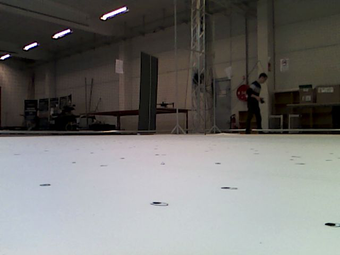
\includegraphics[width=\textwidth]{figure/tsne_random/D/8.png}
      \caption{Cluster D - real}
   \end{subfigure}
   \begin{subfigure}{0.29\textwidth}
      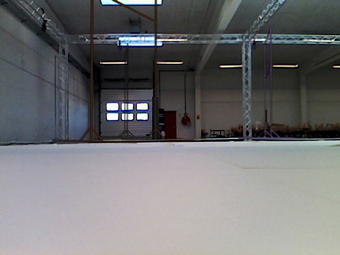
\includegraphics[width=\textwidth]{figure/tsne_random/D/9.png}
      \caption{Cluster D - synthetic}
   \end{subfigure}
   \begin{subfigure}{0.29\textwidth}
      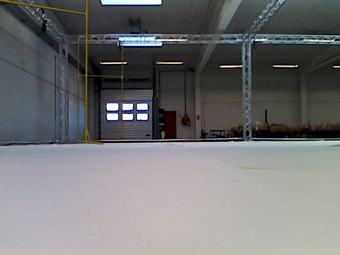
\includegraphics[width=\textwidth]{figure/tsne_random/D/4.png}
      \caption{Cluster D - synthetic}
   \end{subfigure}

   \begin{subfigure}{0.29\textwidth}
      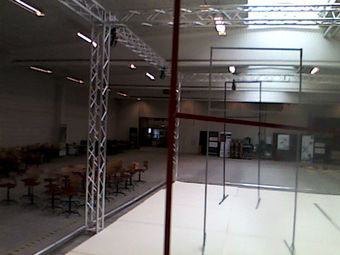
\includegraphics[width=\textwidth]{figure/tsne_random/F/1.png}
      \caption{Cluster F - real}
   \end{subfigure}
   \begin{subfigure}{0.29\textwidth}
      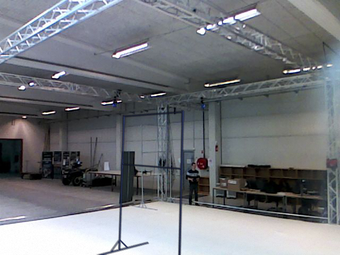
\includegraphics[width=\textwidth]{figure/tsne_random/F/9.png}
      \caption{Cluster F - synthetic}
   \end{subfigure}
   \begin{subfigure}{0.29\textwidth}
      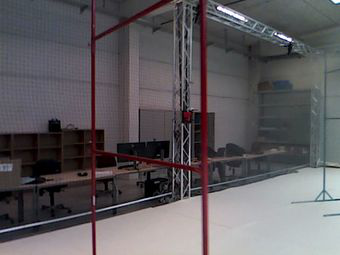
\includegraphics[width=\textwidth]{figure/tsne_random/F/6.png}
      \caption{Cluster F - real}
   \end{subfigure}
   \caption[Synthetic versus real images comparison]{Images from clusters D and
   F are randomly picked and shown as a comparison.}
   \label{fig:clustering}
\end{figure}

Furthermore, this analysis is made on a random selection of samples, which is
not well balanced due to the fact that each batch of synthetic images shows
roughly 70\% of gates visibility, while the real test set -- being a lot less
random -- is probably closer to 100\%. To get rid of these disparities and
offer a fairer comparison, another t-SNE analysis, this time applied to
hand-picked samples, is shown in figure~\ref{fig:tsne-manual}. Those manually
selected samples represent similar configurations of gate placement and
points of view, and intend to eliminate cases where no gates are visible. In
the end, 30 samples were manually selected from each dataset, and the result is
a much more homogeneous plot after the t-SNE analysis.

\begin{figure}[h!]
	\centering
	\begin{subfigure}[h]{0.49\textwidth}
		\scalebox{0.4}{
			%% Creator: Matplotlib, PGF backend
%%
%% To include the figure in your LaTeX document, write
%%   \input{<filename>.pgf}
%%
%% Make sure the required packages are loaded in your preamble
%%   \usepackage{pgf}
%%
%% Figures using additional raster images can only be included by \input if
%% they are in the same directory as the main LaTeX file. For loading figures
%% from other directories you can use the `import` package
%%   \usepackage{import}
%% and then include the figures with
%%   \import{<path to file>}{<filename>.pgf}
%%
%% Matplotlib used the following preamble
%%
\begingroup%
\makeatletter%
\begin{pgfpicture}%
\pgfpathrectangle{\pgfpointorigin}{\pgfqpoint{8.000000in}{6.000000in}}%
\pgfusepath{use as bounding box, clip}%
\begin{pgfscope}%
\pgfsetbuttcap%
\pgfsetmiterjoin%
\definecolor{currentfill}{rgb}{1.000000,1.000000,1.000000}%
\pgfsetfillcolor{currentfill}%
\pgfsetlinewidth{0.000000pt}%
\definecolor{currentstroke}{rgb}{1.000000,1.000000,1.000000}%
\pgfsetstrokecolor{currentstroke}%
\pgfsetdash{}{0pt}%
\pgfpathmoveto{\pgfqpoint{0.000000in}{0.000000in}}%
\pgfpathlineto{\pgfqpoint{8.000000in}{0.000000in}}%
\pgfpathlineto{\pgfqpoint{8.000000in}{6.000000in}}%
\pgfpathlineto{\pgfqpoint{0.000000in}{6.000000in}}%
\pgfpathclose%
\pgfusepath{fill}%
\end{pgfscope}%
\begin{pgfscope}%
\pgfsetbuttcap%
\pgfsetmiterjoin%
\definecolor{currentfill}{rgb}{1.000000,1.000000,1.000000}%
\pgfsetfillcolor{currentfill}%
\pgfsetlinewidth{0.000000pt}%
\definecolor{currentstroke}{rgb}{0.000000,0.000000,0.000000}%
\pgfsetstrokecolor{currentstroke}%
\pgfsetstrokeopacity{0.000000}%
\pgfsetdash{}{0pt}%
\pgfpathmoveto{\pgfqpoint{1.000000in}{0.600000in}}%
\pgfpathlineto{\pgfqpoint{7.200000in}{0.600000in}}%
\pgfpathlineto{\pgfqpoint{7.200000in}{5.400000in}}%
\pgfpathlineto{\pgfqpoint{1.000000in}{5.400000in}}%
\pgfpathclose%
\pgfusepath{fill}%
\end{pgfscope}%
\begin{pgfscope}%
\pgfpathrectangle{\pgfqpoint{1.000000in}{0.600000in}}{\pgfqpoint{6.200000in}{4.800000in}} %
\pgfusepath{clip}%
\pgfsetbuttcap%
\pgfsetroundjoin%
\definecolor{currentfill}{rgb}{1.000000,0.000000,0.000000}%
\pgfsetfillcolor{currentfill}%
\pgfsetlinewidth{1.003750pt}%
\definecolor{currentstroke}{rgb}{0.000000,0.000000,0.000000}%
\pgfsetstrokecolor{currentstroke}%
\pgfsetdash{}{0pt}%
\pgfpathmoveto{\pgfqpoint{5.282767in}{3.784678in}}%
\pgfpathcurveto{\pgfqpoint{5.291003in}{3.784678in}}{\pgfqpoint{5.298903in}{3.787950in}}{\pgfqpoint{5.304727in}{3.793774in}}%
\pgfpathcurveto{\pgfqpoint{5.310551in}{3.799598in}}{\pgfqpoint{5.313823in}{3.807498in}}{\pgfqpoint{5.313823in}{3.815734in}}%
\pgfpathcurveto{\pgfqpoint{5.313823in}{3.823971in}}{\pgfqpoint{5.310551in}{3.831871in}}{\pgfqpoint{5.304727in}{3.837695in}}%
\pgfpathcurveto{\pgfqpoint{5.298903in}{3.843519in}}{\pgfqpoint{5.291003in}{3.846791in}}{\pgfqpoint{5.282767in}{3.846791in}}%
\pgfpathcurveto{\pgfqpoint{5.274530in}{3.846791in}}{\pgfqpoint{5.266630in}{3.843519in}}{\pgfqpoint{5.260807in}{3.837695in}}%
\pgfpathcurveto{\pgfqpoint{5.254983in}{3.831871in}}{\pgfqpoint{5.251710in}{3.823971in}}{\pgfqpoint{5.251710in}{3.815734in}}%
\pgfpathcurveto{\pgfqpoint{5.251710in}{3.807498in}}{\pgfqpoint{5.254983in}{3.799598in}}{\pgfqpoint{5.260807in}{3.793774in}}%
\pgfpathcurveto{\pgfqpoint{5.266630in}{3.787950in}}{\pgfqpoint{5.274530in}{3.784678in}}{\pgfqpoint{5.282767in}{3.784678in}}%
\pgfpathclose%
\pgfusepath{stroke,fill}%
\end{pgfscope}%
\begin{pgfscope}%
\pgfpathrectangle{\pgfqpoint{1.000000in}{0.600000in}}{\pgfqpoint{6.200000in}{4.800000in}} %
\pgfusepath{clip}%
\pgfsetbuttcap%
\pgfsetroundjoin%
\definecolor{currentfill}{rgb}{1.000000,0.000000,0.000000}%
\pgfsetfillcolor{currentfill}%
\pgfsetlinewidth{1.003750pt}%
\definecolor{currentstroke}{rgb}{0.000000,0.000000,0.000000}%
\pgfsetstrokecolor{currentstroke}%
\pgfsetdash{}{0pt}%
\pgfpathmoveto{\pgfqpoint{2.370422in}{2.636279in}}%
\pgfpathcurveto{\pgfqpoint{2.378659in}{2.636279in}}{\pgfqpoint{2.386559in}{2.639551in}}{\pgfqpoint{2.392383in}{2.645375in}}%
\pgfpathcurveto{\pgfqpoint{2.398207in}{2.651199in}}{\pgfqpoint{2.401479in}{2.659099in}}{\pgfqpoint{2.401479in}{2.667335in}}%
\pgfpathcurveto{\pgfqpoint{2.401479in}{2.675572in}}{\pgfqpoint{2.398207in}{2.683472in}}{\pgfqpoint{2.392383in}{2.689296in}}%
\pgfpathcurveto{\pgfqpoint{2.386559in}{2.695120in}}{\pgfqpoint{2.378659in}{2.698392in}}{\pgfqpoint{2.370422in}{2.698392in}}%
\pgfpathcurveto{\pgfqpoint{2.362186in}{2.698392in}}{\pgfqpoint{2.354286in}{2.695120in}}{\pgfqpoint{2.348462in}{2.689296in}}%
\pgfpathcurveto{\pgfqpoint{2.342638in}{2.683472in}}{\pgfqpoint{2.339366in}{2.675572in}}{\pgfqpoint{2.339366in}{2.667335in}}%
\pgfpathcurveto{\pgfqpoint{2.339366in}{2.659099in}}{\pgfqpoint{2.342638in}{2.651199in}}{\pgfqpoint{2.348462in}{2.645375in}}%
\pgfpathcurveto{\pgfqpoint{2.354286in}{2.639551in}}{\pgfqpoint{2.362186in}{2.636279in}}{\pgfqpoint{2.370422in}{2.636279in}}%
\pgfpathclose%
\pgfusepath{stroke,fill}%
\end{pgfscope}%
\begin{pgfscope}%
\pgfpathrectangle{\pgfqpoint{1.000000in}{0.600000in}}{\pgfqpoint{6.200000in}{4.800000in}} %
\pgfusepath{clip}%
\pgfsetbuttcap%
\pgfsetroundjoin%
\definecolor{currentfill}{rgb}{1.000000,0.000000,0.000000}%
\pgfsetfillcolor{currentfill}%
\pgfsetlinewidth{1.003750pt}%
\definecolor{currentstroke}{rgb}{0.000000,0.000000,0.000000}%
\pgfsetstrokecolor{currentstroke}%
\pgfsetdash{}{0pt}%
\pgfpathmoveto{\pgfqpoint{2.891460in}{4.829130in}}%
\pgfpathcurveto{\pgfqpoint{2.899696in}{4.829130in}}{\pgfqpoint{2.907596in}{4.832402in}}{\pgfqpoint{2.913420in}{4.838226in}}%
\pgfpathcurveto{\pgfqpoint{2.919244in}{4.844050in}}{\pgfqpoint{2.922516in}{4.851950in}}{\pgfqpoint{2.922516in}{4.860186in}}%
\pgfpathcurveto{\pgfqpoint{2.922516in}{4.868422in}}{\pgfqpoint{2.919244in}{4.876323in}}{\pgfqpoint{2.913420in}{4.882146in}}%
\pgfpathcurveto{\pgfqpoint{2.907596in}{4.887970in}}{\pgfqpoint{2.899696in}{4.891243in}}{\pgfqpoint{2.891460in}{4.891243in}}%
\pgfpathcurveto{\pgfqpoint{2.883223in}{4.891243in}}{\pgfqpoint{2.875323in}{4.887970in}}{\pgfqpoint{2.869499in}{4.882146in}}%
\pgfpathcurveto{\pgfqpoint{2.863675in}{4.876323in}}{\pgfqpoint{2.860403in}{4.868422in}}{\pgfqpoint{2.860403in}{4.860186in}}%
\pgfpathcurveto{\pgfqpoint{2.860403in}{4.851950in}}{\pgfqpoint{2.863675in}{4.844050in}}{\pgfqpoint{2.869499in}{4.838226in}}%
\pgfpathcurveto{\pgfqpoint{2.875323in}{4.832402in}}{\pgfqpoint{2.883223in}{4.829130in}}{\pgfqpoint{2.891460in}{4.829130in}}%
\pgfpathclose%
\pgfusepath{stroke,fill}%
\end{pgfscope}%
\begin{pgfscope}%
\pgfpathrectangle{\pgfqpoint{1.000000in}{0.600000in}}{\pgfqpoint{6.200000in}{4.800000in}} %
\pgfusepath{clip}%
\pgfsetbuttcap%
\pgfsetroundjoin%
\definecolor{currentfill}{rgb}{1.000000,0.000000,0.000000}%
\pgfsetfillcolor{currentfill}%
\pgfsetlinewidth{1.003750pt}%
\definecolor{currentstroke}{rgb}{0.000000,0.000000,0.000000}%
\pgfsetstrokecolor{currentstroke}%
\pgfsetdash{}{0pt}%
\pgfpathmoveto{\pgfqpoint{4.659051in}{2.066233in}}%
\pgfpathcurveto{\pgfqpoint{4.667287in}{2.066233in}}{\pgfqpoint{4.675187in}{2.069505in}}{\pgfqpoint{4.681011in}{2.075329in}}%
\pgfpathcurveto{\pgfqpoint{4.686835in}{2.081153in}}{\pgfqpoint{4.690107in}{2.089053in}}{\pgfqpoint{4.690107in}{2.097289in}}%
\pgfpathcurveto{\pgfqpoint{4.690107in}{2.105525in}}{\pgfqpoint{4.686835in}{2.113425in}}{\pgfqpoint{4.681011in}{2.119249in}}%
\pgfpathcurveto{\pgfqpoint{4.675187in}{2.125073in}}{\pgfqpoint{4.667287in}{2.128346in}}{\pgfqpoint{4.659051in}{2.128346in}}%
\pgfpathcurveto{\pgfqpoint{4.650814in}{2.128346in}}{\pgfqpoint{4.642914in}{2.125073in}}{\pgfqpoint{4.637090in}{2.119249in}}%
\pgfpathcurveto{\pgfqpoint{4.631267in}{2.113425in}}{\pgfqpoint{4.627994in}{2.105525in}}{\pgfqpoint{4.627994in}{2.097289in}}%
\pgfpathcurveto{\pgfqpoint{4.627994in}{2.089053in}}{\pgfqpoint{4.631267in}{2.081153in}}{\pgfqpoint{4.637090in}{2.075329in}}%
\pgfpathcurveto{\pgfqpoint{4.642914in}{2.069505in}}{\pgfqpoint{4.650814in}{2.066233in}}{\pgfqpoint{4.659051in}{2.066233in}}%
\pgfpathclose%
\pgfusepath{stroke,fill}%
\end{pgfscope}%
\begin{pgfscope}%
\pgfpathrectangle{\pgfqpoint{1.000000in}{0.600000in}}{\pgfqpoint{6.200000in}{4.800000in}} %
\pgfusepath{clip}%
\pgfsetbuttcap%
\pgfsetroundjoin%
\definecolor{currentfill}{rgb}{1.000000,0.000000,0.000000}%
\pgfsetfillcolor{currentfill}%
\pgfsetlinewidth{1.003750pt}%
\definecolor{currentstroke}{rgb}{0.000000,0.000000,0.000000}%
\pgfsetstrokecolor{currentstroke}%
\pgfsetdash{}{0pt}%
\pgfpathmoveto{\pgfqpoint{3.044069in}{4.589249in}}%
\pgfpathcurveto{\pgfqpoint{3.052305in}{4.589249in}}{\pgfqpoint{3.060205in}{4.592522in}}{\pgfqpoint{3.066029in}{4.598346in}}%
\pgfpathcurveto{\pgfqpoint{3.071853in}{4.604170in}}{\pgfqpoint{3.075125in}{4.612070in}}{\pgfqpoint{3.075125in}{4.620306in}}%
\pgfpathcurveto{\pgfqpoint{3.075125in}{4.628542in}}{\pgfqpoint{3.071853in}{4.636442in}}{\pgfqpoint{3.066029in}{4.642266in}}%
\pgfpathcurveto{\pgfqpoint{3.060205in}{4.648090in}}{\pgfqpoint{3.052305in}{4.651362in}}{\pgfqpoint{3.044069in}{4.651362in}}%
\pgfpathcurveto{\pgfqpoint{3.035832in}{4.651362in}}{\pgfqpoint{3.027932in}{4.648090in}}{\pgfqpoint{3.022108in}{4.642266in}}%
\pgfpathcurveto{\pgfqpoint{3.016284in}{4.636442in}}{\pgfqpoint{3.013012in}{4.628542in}}{\pgfqpoint{3.013012in}{4.620306in}}%
\pgfpathcurveto{\pgfqpoint{3.013012in}{4.612070in}}{\pgfqpoint{3.016284in}{4.604170in}}{\pgfqpoint{3.022108in}{4.598346in}}%
\pgfpathcurveto{\pgfqpoint{3.027932in}{4.592522in}}{\pgfqpoint{3.035832in}{4.589249in}}{\pgfqpoint{3.044069in}{4.589249in}}%
\pgfpathclose%
\pgfusepath{stroke,fill}%
\end{pgfscope}%
\begin{pgfscope}%
\pgfpathrectangle{\pgfqpoint{1.000000in}{0.600000in}}{\pgfqpoint{6.200000in}{4.800000in}} %
\pgfusepath{clip}%
\pgfsetbuttcap%
\pgfsetroundjoin%
\definecolor{currentfill}{rgb}{1.000000,0.000000,0.000000}%
\pgfsetfillcolor{currentfill}%
\pgfsetlinewidth{1.003750pt}%
\definecolor{currentstroke}{rgb}{0.000000,0.000000,0.000000}%
\pgfsetstrokecolor{currentstroke}%
\pgfsetdash{}{0pt}%
\pgfpathmoveto{\pgfqpoint{3.849910in}{4.351300in}}%
\pgfpathcurveto{\pgfqpoint{3.858146in}{4.351300in}}{\pgfqpoint{3.866046in}{4.354572in}}{\pgfqpoint{3.871870in}{4.360396in}}%
\pgfpathcurveto{\pgfqpoint{3.877694in}{4.366220in}}{\pgfqpoint{3.880966in}{4.374120in}}{\pgfqpoint{3.880966in}{4.382356in}}%
\pgfpathcurveto{\pgfqpoint{3.880966in}{4.390592in}}{\pgfqpoint{3.877694in}{4.398493in}}{\pgfqpoint{3.871870in}{4.404316in}}%
\pgfpathcurveto{\pgfqpoint{3.866046in}{4.410140in}}{\pgfqpoint{3.858146in}{4.413413in}}{\pgfqpoint{3.849910in}{4.413413in}}%
\pgfpathcurveto{\pgfqpoint{3.841674in}{4.413413in}}{\pgfqpoint{3.833774in}{4.410140in}}{\pgfqpoint{3.827950in}{4.404316in}}%
\pgfpathcurveto{\pgfqpoint{3.822126in}{4.398493in}}{\pgfqpoint{3.818853in}{4.390592in}}{\pgfqpoint{3.818853in}{4.382356in}}%
\pgfpathcurveto{\pgfqpoint{3.818853in}{4.374120in}}{\pgfqpoint{3.822126in}{4.366220in}}{\pgfqpoint{3.827950in}{4.360396in}}%
\pgfpathcurveto{\pgfqpoint{3.833774in}{4.354572in}}{\pgfqpoint{3.841674in}{4.351300in}}{\pgfqpoint{3.849910in}{4.351300in}}%
\pgfpathclose%
\pgfusepath{stroke,fill}%
\end{pgfscope}%
\begin{pgfscope}%
\pgfpathrectangle{\pgfqpoint{1.000000in}{0.600000in}}{\pgfqpoint{6.200000in}{4.800000in}} %
\pgfusepath{clip}%
\pgfsetbuttcap%
\pgfsetroundjoin%
\definecolor{currentfill}{rgb}{1.000000,0.000000,0.000000}%
\pgfsetfillcolor{currentfill}%
\pgfsetlinewidth{1.003750pt}%
\definecolor{currentstroke}{rgb}{0.000000,0.000000,0.000000}%
\pgfsetstrokecolor{currentstroke}%
\pgfsetdash{}{0pt}%
\pgfpathmoveto{\pgfqpoint{4.036969in}{3.377574in}}%
\pgfpathcurveto{\pgfqpoint{4.045205in}{3.377574in}}{\pgfqpoint{4.053105in}{3.380846in}}{\pgfqpoint{4.058929in}{3.386670in}}%
\pgfpathcurveto{\pgfqpoint{4.064753in}{3.392494in}}{\pgfqpoint{4.068025in}{3.400394in}}{\pgfqpoint{4.068025in}{3.408630in}}%
\pgfpathcurveto{\pgfqpoint{4.068025in}{3.416866in}}{\pgfqpoint{4.064753in}{3.424766in}}{\pgfqpoint{4.058929in}{3.430590in}}%
\pgfpathcurveto{\pgfqpoint{4.053105in}{3.436414in}}{\pgfqpoint{4.045205in}{3.439687in}}{\pgfqpoint{4.036969in}{3.439687in}}%
\pgfpathcurveto{\pgfqpoint{4.028733in}{3.439687in}}{\pgfqpoint{4.020833in}{3.436414in}}{\pgfqpoint{4.015009in}{3.430590in}}%
\pgfpathcurveto{\pgfqpoint{4.009185in}{3.424766in}}{\pgfqpoint{4.005912in}{3.416866in}}{\pgfqpoint{4.005912in}{3.408630in}}%
\pgfpathcurveto{\pgfqpoint{4.005912in}{3.400394in}}{\pgfqpoint{4.009185in}{3.392494in}}{\pgfqpoint{4.015009in}{3.386670in}}%
\pgfpathcurveto{\pgfqpoint{4.020833in}{3.380846in}}{\pgfqpoint{4.028733in}{3.377574in}}{\pgfqpoint{4.036969in}{3.377574in}}%
\pgfpathclose%
\pgfusepath{stroke,fill}%
\end{pgfscope}%
\begin{pgfscope}%
\pgfpathrectangle{\pgfqpoint{1.000000in}{0.600000in}}{\pgfqpoint{6.200000in}{4.800000in}} %
\pgfusepath{clip}%
\pgfsetbuttcap%
\pgfsetroundjoin%
\definecolor{currentfill}{rgb}{1.000000,0.000000,0.000000}%
\pgfsetfillcolor{currentfill}%
\pgfsetlinewidth{1.003750pt}%
\definecolor{currentstroke}{rgb}{0.000000,0.000000,0.000000}%
\pgfsetstrokecolor{currentstroke}%
\pgfsetdash{}{0pt}%
\pgfpathmoveto{\pgfqpoint{4.991105in}{2.666711in}}%
\pgfpathcurveto{\pgfqpoint{4.999342in}{2.666711in}}{\pgfqpoint{5.007242in}{2.669984in}}{\pgfqpoint{5.013066in}{2.675808in}}%
\pgfpathcurveto{\pgfqpoint{5.018890in}{2.681631in}}{\pgfqpoint{5.022162in}{2.689532in}}{\pgfqpoint{5.022162in}{2.697768in}}%
\pgfpathcurveto{\pgfqpoint{5.022162in}{2.706004in}}{\pgfqpoint{5.018890in}{2.713904in}}{\pgfqpoint{5.013066in}{2.719728in}}%
\pgfpathcurveto{\pgfqpoint{5.007242in}{2.725552in}}{\pgfqpoint{4.999342in}{2.728824in}}{\pgfqpoint{4.991105in}{2.728824in}}%
\pgfpathcurveto{\pgfqpoint{4.982869in}{2.728824in}}{\pgfqpoint{4.974969in}{2.725552in}}{\pgfqpoint{4.969145in}{2.719728in}}%
\pgfpathcurveto{\pgfqpoint{4.963321in}{2.713904in}}{\pgfqpoint{4.960049in}{2.706004in}}{\pgfqpoint{4.960049in}{2.697768in}}%
\pgfpathcurveto{\pgfqpoint{4.960049in}{2.689532in}}{\pgfqpoint{4.963321in}{2.681631in}}{\pgfqpoint{4.969145in}{2.675808in}}%
\pgfpathcurveto{\pgfqpoint{4.974969in}{2.669984in}}{\pgfqpoint{4.982869in}{2.666711in}}{\pgfqpoint{4.991105in}{2.666711in}}%
\pgfpathclose%
\pgfusepath{stroke,fill}%
\end{pgfscope}%
\begin{pgfscope}%
\pgfpathrectangle{\pgfqpoint{1.000000in}{0.600000in}}{\pgfqpoint{6.200000in}{4.800000in}} %
\pgfusepath{clip}%
\pgfsetbuttcap%
\pgfsetroundjoin%
\definecolor{currentfill}{rgb}{1.000000,0.000000,0.000000}%
\pgfsetfillcolor{currentfill}%
\pgfsetlinewidth{1.003750pt}%
\definecolor{currentstroke}{rgb}{0.000000,0.000000,0.000000}%
\pgfsetstrokecolor{currentstroke}%
\pgfsetdash{}{0pt}%
\pgfpathmoveto{\pgfqpoint{3.360564in}{2.538571in}}%
\pgfpathcurveto{\pgfqpoint{3.368800in}{2.538571in}}{\pgfqpoint{3.376700in}{2.541844in}}{\pgfqpoint{3.382524in}{2.547668in}}%
\pgfpathcurveto{\pgfqpoint{3.388348in}{2.553492in}}{\pgfqpoint{3.391620in}{2.561392in}}{\pgfqpoint{3.391620in}{2.569628in}}%
\pgfpathcurveto{\pgfqpoint{3.391620in}{2.577864in}}{\pgfqpoint{3.388348in}{2.585764in}}{\pgfqpoint{3.382524in}{2.591588in}}%
\pgfpathcurveto{\pgfqpoint{3.376700in}{2.597412in}}{\pgfqpoint{3.368800in}{2.600684in}}{\pgfqpoint{3.360564in}{2.600684in}}%
\pgfpathcurveto{\pgfqpoint{3.352327in}{2.600684in}}{\pgfqpoint{3.344427in}{2.597412in}}{\pgfqpoint{3.338603in}{2.591588in}}%
\pgfpathcurveto{\pgfqpoint{3.332779in}{2.585764in}}{\pgfqpoint{3.329507in}{2.577864in}}{\pgfqpoint{3.329507in}{2.569628in}}%
\pgfpathcurveto{\pgfqpoint{3.329507in}{2.561392in}}{\pgfqpoint{3.332779in}{2.553492in}}{\pgfqpoint{3.338603in}{2.547668in}}%
\pgfpathcurveto{\pgfqpoint{3.344427in}{2.541844in}}{\pgfqpoint{3.352327in}{2.538571in}}{\pgfqpoint{3.360564in}{2.538571in}}%
\pgfpathclose%
\pgfusepath{stroke,fill}%
\end{pgfscope}%
\begin{pgfscope}%
\pgfpathrectangle{\pgfqpoint{1.000000in}{0.600000in}}{\pgfqpoint{6.200000in}{4.800000in}} %
\pgfusepath{clip}%
\pgfsetbuttcap%
\pgfsetroundjoin%
\definecolor{currentfill}{rgb}{1.000000,0.000000,0.000000}%
\pgfsetfillcolor{currentfill}%
\pgfsetlinewidth{1.003750pt}%
\definecolor{currentstroke}{rgb}{0.000000,0.000000,0.000000}%
\pgfsetstrokecolor{currentstroke}%
\pgfsetdash{}{0pt}%
\pgfpathmoveto{\pgfqpoint{4.422378in}{4.747298in}}%
\pgfpathcurveto{\pgfqpoint{4.430614in}{4.747298in}}{\pgfqpoint{4.438514in}{4.750570in}}{\pgfqpoint{4.444338in}{4.756394in}}%
\pgfpathcurveto{\pgfqpoint{4.450162in}{4.762218in}}{\pgfqpoint{4.453434in}{4.770118in}}{\pgfqpoint{4.453434in}{4.778354in}}%
\pgfpathcurveto{\pgfqpoint{4.453434in}{4.786591in}}{\pgfqpoint{4.450162in}{4.794491in}}{\pgfqpoint{4.444338in}{4.800315in}}%
\pgfpathcurveto{\pgfqpoint{4.438514in}{4.806139in}}{\pgfqpoint{4.430614in}{4.809411in}}{\pgfqpoint{4.422378in}{4.809411in}}%
\pgfpathcurveto{\pgfqpoint{4.414141in}{4.809411in}}{\pgfqpoint{4.406241in}{4.806139in}}{\pgfqpoint{4.400417in}{4.800315in}}%
\pgfpathcurveto{\pgfqpoint{4.394593in}{4.794491in}}{\pgfqpoint{4.391321in}{4.786591in}}{\pgfqpoint{4.391321in}{4.778354in}}%
\pgfpathcurveto{\pgfqpoint{4.391321in}{4.770118in}}{\pgfqpoint{4.394593in}{4.762218in}}{\pgfqpoint{4.400417in}{4.756394in}}%
\pgfpathcurveto{\pgfqpoint{4.406241in}{4.750570in}}{\pgfqpoint{4.414141in}{4.747298in}}{\pgfqpoint{4.422378in}{4.747298in}}%
\pgfpathclose%
\pgfusepath{stroke,fill}%
\end{pgfscope}%
\begin{pgfscope}%
\pgfpathrectangle{\pgfqpoint{1.000000in}{0.600000in}}{\pgfqpoint{6.200000in}{4.800000in}} %
\pgfusepath{clip}%
\pgfsetbuttcap%
\pgfsetroundjoin%
\definecolor{currentfill}{rgb}{1.000000,0.000000,0.000000}%
\pgfsetfillcolor{currentfill}%
\pgfsetlinewidth{1.003750pt}%
\definecolor{currentstroke}{rgb}{0.000000,0.000000,0.000000}%
\pgfsetstrokecolor{currentstroke}%
\pgfsetdash{}{0pt}%
\pgfpathmoveto{\pgfqpoint{3.364060in}{3.460985in}}%
\pgfpathcurveto{\pgfqpoint{3.372297in}{3.460985in}}{\pgfqpoint{3.380197in}{3.464257in}}{\pgfqpoint{3.386021in}{3.470081in}}%
\pgfpathcurveto{\pgfqpoint{3.391844in}{3.475905in}}{\pgfqpoint{3.395117in}{3.483805in}}{\pgfqpoint{3.395117in}{3.492042in}}%
\pgfpathcurveto{\pgfqpoint{3.395117in}{3.500278in}}{\pgfqpoint{3.391844in}{3.508178in}}{\pgfqpoint{3.386021in}{3.514002in}}%
\pgfpathcurveto{\pgfqpoint{3.380197in}{3.519826in}}{\pgfqpoint{3.372297in}{3.523098in}}{\pgfqpoint{3.364060in}{3.523098in}}%
\pgfpathcurveto{\pgfqpoint{3.355824in}{3.523098in}}{\pgfqpoint{3.347924in}{3.519826in}}{\pgfqpoint{3.342100in}{3.514002in}}%
\pgfpathcurveto{\pgfqpoint{3.336276in}{3.508178in}}{\pgfqpoint{3.333004in}{3.500278in}}{\pgfqpoint{3.333004in}{3.492042in}}%
\pgfpathcurveto{\pgfqpoint{3.333004in}{3.483805in}}{\pgfqpoint{3.336276in}{3.475905in}}{\pgfqpoint{3.342100in}{3.470081in}}%
\pgfpathcurveto{\pgfqpoint{3.347924in}{3.464257in}}{\pgfqpoint{3.355824in}{3.460985in}}{\pgfqpoint{3.364060in}{3.460985in}}%
\pgfpathclose%
\pgfusepath{stroke,fill}%
\end{pgfscope}%
\begin{pgfscope}%
\pgfpathrectangle{\pgfqpoint{1.000000in}{0.600000in}}{\pgfqpoint{6.200000in}{4.800000in}} %
\pgfusepath{clip}%
\pgfsetbuttcap%
\pgfsetroundjoin%
\definecolor{currentfill}{rgb}{1.000000,0.000000,0.000000}%
\pgfsetfillcolor{currentfill}%
\pgfsetlinewidth{1.003750pt}%
\definecolor{currentstroke}{rgb}{0.000000,0.000000,0.000000}%
\pgfsetstrokecolor{currentstroke}%
\pgfsetdash{}{0pt}%
\pgfpathmoveto{\pgfqpoint{2.262233in}{4.020715in}}%
\pgfpathcurveto{\pgfqpoint{2.270470in}{4.020715in}}{\pgfqpoint{2.278370in}{4.023987in}}{\pgfqpoint{2.284194in}{4.029811in}}%
\pgfpathcurveto{\pgfqpoint{2.290018in}{4.035635in}}{\pgfqpoint{2.293290in}{4.043535in}}{\pgfqpoint{2.293290in}{4.051771in}}%
\pgfpathcurveto{\pgfqpoint{2.293290in}{4.060008in}}{\pgfqpoint{2.290018in}{4.067908in}}{\pgfqpoint{2.284194in}{4.073732in}}%
\pgfpathcurveto{\pgfqpoint{2.278370in}{4.079556in}}{\pgfqpoint{2.270470in}{4.082828in}}{\pgfqpoint{2.262233in}{4.082828in}}%
\pgfpathcurveto{\pgfqpoint{2.253997in}{4.082828in}}{\pgfqpoint{2.246097in}{4.079556in}}{\pgfqpoint{2.240273in}{4.073732in}}%
\pgfpathcurveto{\pgfqpoint{2.234449in}{4.067908in}}{\pgfqpoint{2.231177in}{4.060008in}}{\pgfqpoint{2.231177in}{4.051771in}}%
\pgfpathcurveto{\pgfqpoint{2.231177in}{4.043535in}}{\pgfqpoint{2.234449in}{4.035635in}}{\pgfqpoint{2.240273in}{4.029811in}}%
\pgfpathcurveto{\pgfqpoint{2.246097in}{4.023987in}}{\pgfqpoint{2.253997in}{4.020715in}}{\pgfqpoint{2.262233in}{4.020715in}}%
\pgfpathclose%
\pgfusepath{stroke,fill}%
\end{pgfscope}%
\begin{pgfscope}%
\pgfpathrectangle{\pgfqpoint{1.000000in}{0.600000in}}{\pgfqpoint{6.200000in}{4.800000in}} %
\pgfusepath{clip}%
\pgfsetbuttcap%
\pgfsetroundjoin%
\definecolor{currentfill}{rgb}{1.000000,0.000000,0.000000}%
\pgfsetfillcolor{currentfill}%
\pgfsetlinewidth{1.003750pt}%
\definecolor{currentstroke}{rgb}{0.000000,0.000000,0.000000}%
\pgfsetstrokecolor{currentstroke}%
\pgfsetdash{}{0pt}%
\pgfpathmoveto{\pgfqpoint{2.860565in}{2.106659in}}%
\pgfpathcurveto{\pgfqpoint{2.868802in}{2.106659in}}{\pgfqpoint{2.876702in}{2.109931in}}{\pgfqpoint{2.882526in}{2.115755in}}%
\pgfpathcurveto{\pgfqpoint{2.888350in}{2.121579in}}{\pgfqpoint{2.891622in}{2.129479in}}{\pgfqpoint{2.891622in}{2.137715in}}%
\pgfpathcurveto{\pgfqpoint{2.891622in}{2.145952in}}{\pgfqpoint{2.888350in}{2.153852in}}{\pgfqpoint{2.882526in}{2.159676in}}%
\pgfpathcurveto{\pgfqpoint{2.876702in}{2.165499in}}{\pgfqpoint{2.868802in}{2.168772in}}{\pgfqpoint{2.860565in}{2.168772in}}%
\pgfpathcurveto{\pgfqpoint{2.852329in}{2.168772in}}{\pgfqpoint{2.844429in}{2.165499in}}{\pgfqpoint{2.838605in}{2.159676in}}%
\pgfpathcurveto{\pgfqpoint{2.832781in}{2.153852in}}{\pgfqpoint{2.829509in}{2.145952in}}{\pgfqpoint{2.829509in}{2.137715in}}%
\pgfpathcurveto{\pgfqpoint{2.829509in}{2.129479in}}{\pgfqpoint{2.832781in}{2.121579in}}{\pgfqpoint{2.838605in}{2.115755in}}%
\pgfpathcurveto{\pgfqpoint{2.844429in}{2.109931in}}{\pgfqpoint{2.852329in}{2.106659in}}{\pgfqpoint{2.860565in}{2.106659in}}%
\pgfpathclose%
\pgfusepath{stroke,fill}%
\end{pgfscope}%
\begin{pgfscope}%
\pgfpathrectangle{\pgfqpoint{1.000000in}{0.600000in}}{\pgfqpoint{6.200000in}{4.800000in}} %
\pgfusepath{clip}%
\pgfsetbuttcap%
\pgfsetroundjoin%
\definecolor{currentfill}{rgb}{1.000000,0.000000,0.000000}%
\pgfsetfillcolor{currentfill}%
\pgfsetlinewidth{1.003750pt}%
\definecolor{currentstroke}{rgb}{0.000000,0.000000,0.000000}%
\pgfsetstrokecolor{currentstroke}%
\pgfsetdash{}{0pt}%
\pgfpathmoveto{\pgfqpoint{4.647926in}{3.571446in}}%
\pgfpathcurveto{\pgfqpoint{4.656163in}{3.571446in}}{\pgfqpoint{4.664063in}{3.574719in}}{\pgfqpoint{4.669887in}{3.580543in}}%
\pgfpathcurveto{\pgfqpoint{4.675711in}{3.586367in}}{\pgfqpoint{4.678983in}{3.594267in}}{\pgfqpoint{4.678983in}{3.602503in}}%
\pgfpathcurveto{\pgfqpoint{4.678983in}{3.610739in}}{\pgfqpoint{4.675711in}{3.618639in}}{\pgfqpoint{4.669887in}{3.624463in}}%
\pgfpathcurveto{\pgfqpoint{4.664063in}{3.630287in}}{\pgfqpoint{4.656163in}{3.633559in}}{\pgfqpoint{4.647926in}{3.633559in}}%
\pgfpathcurveto{\pgfqpoint{4.639690in}{3.633559in}}{\pgfqpoint{4.631790in}{3.630287in}}{\pgfqpoint{4.625966in}{3.624463in}}%
\pgfpathcurveto{\pgfqpoint{4.620142in}{3.618639in}}{\pgfqpoint{4.616870in}{3.610739in}}{\pgfqpoint{4.616870in}{3.602503in}}%
\pgfpathcurveto{\pgfqpoint{4.616870in}{3.594267in}}{\pgfqpoint{4.620142in}{3.586367in}}{\pgfqpoint{4.625966in}{3.580543in}}%
\pgfpathcurveto{\pgfqpoint{4.631790in}{3.574719in}}{\pgfqpoint{4.639690in}{3.571446in}}{\pgfqpoint{4.647926in}{3.571446in}}%
\pgfpathclose%
\pgfusepath{stroke,fill}%
\end{pgfscope}%
\begin{pgfscope}%
\pgfpathrectangle{\pgfqpoint{1.000000in}{0.600000in}}{\pgfqpoint{6.200000in}{4.800000in}} %
\pgfusepath{clip}%
\pgfsetbuttcap%
\pgfsetroundjoin%
\definecolor{currentfill}{rgb}{1.000000,0.000000,0.000000}%
\pgfsetfillcolor{currentfill}%
\pgfsetlinewidth{1.003750pt}%
\definecolor{currentstroke}{rgb}{0.000000,0.000000,0.000000}%
\pgfsetstrokecolor{currentstroke}%
\pgfsetdash{}{0pt}%
\pgfpathmoveto{\pgfqpoint{5.970633in}{4.068280in}}%
\pgfpathcurveto{\pgfqpoint{5.978870in}{4.068280in}}{\pgfqpoint{5.986770in}{4.071552in}}{\pgfqpoint{5.992594in}{4.077376in}}%
\pgfpathcurveto{\pgfqpoint{5.998418in}{4.083200in}}{\pgfqpoint{6.001690in}{4.091100in}}{\pgfqpoint{6.001690in}{4.099336in}}%
\pgfpathcurveto{\pgfqpoint{6.001690in}{4.107572in}}{\pgfqpoint{5.998418in}{4.115472in}}{\pgfqpoint{5.992594in}{4.121296in}}%
\pgfpathcurveto{\pgfqpoint{5.986770in}{4.127120in}}{\pgfqpoint{5.978870in}{4.130393in}}{\pgfqpoint{5.970633in}{4.130393in}}%
\pgfpathcurveto{\pgfqpoint{5.962397in}{4.130393in}}{\pgfqpoint{5.954497in}{4.127120in}}{\pgfqpoint{5.948673in}{4.121296in}}%
\pgfpathcurveto{\pgfqpoint{5.942849in}{4.115472in}}{\pgfqpoint{5.939577in}{4.107572in}}{\pgfqpoint{5.939577in}{4.099336in}}%
\pgfpathcurveto{\pgfqpoint{5.939577in}{4.091100in}}{\pgfqpoint{5.942849in}{4.083200in}}{\pgfqpoint{5.948673in}{4.077376in}}%
\pgfpathcurveto{\pgfqpoint{5.954497in}{4.071552in}}{\pgfqpoint{5.962397in}{4.068280in}}{\pgfqpoint{5.970633in}{4.068280in}}%
\pgfpathclose%
\pgfusepath{stroke,fill}%
\end{pgfscope}%
\begin{pgfscope}%
\pgfpathrectangle{\pgfqpoint{1.000000in}{0.600000in}}{\pgfqpoint{6.200000in}{4.800000in}} %
\pgfusepath{clip}%
\pgfsetbuttcap%
\pgfsetroundjoin%
\definecolor{currentfill}{rgb}{1.000000,0.000000,0.000000}%
\pgfsetfillcolor{currentfill}%
\pgfsetlinewidth{1.003750pt}%
\definecolor{currentstroke}{rgb}{0.000000,0.000000,0.000000}%
\pgfsetstrokecolor{currentstroke}%
\pgfsetdash{}{0pt}%
\pgfpathmoveto{\pgfqpoint{5.536479in}{2.258490in}}%
\pgfpathcurveto{\pgfqpoint{5.544715in}{2.258490in}}{\pgfqpoint{5.552615in}{2.261763in}}{\pgfqpoint{5.558439in}{2.267587in}}%
\pgfpathcurveto{\pgfqpoint{5.564263in}{2.273411in}}{\pgfqpoint{5.567535in}{2.281311in}}{\pgfqpoint{5.567535in}{2.289547in}}%
\pgfpathcurveto{\pgfqpoint{5.567535in}{2.297783in}}{\pgfqpoint{5.564263in}{2.305683in}}{\pgfqpoint{5.558439in}{2.311507in}}%
\pgfpathcurveto{\pgfqpoint{5.552615in}{2.317331in}}{\pgfqpoint{5.544715in}{2.320603in}}{\pgfqpoint{5.536479in}{2.320603in}}%
\pgfpathcurveto{\pgfqpoint{5.528242in}{2.320603in}}{\pgfqpoint{5.520342in}{2.317331in}}{\pgfqpoint{5.514518in}{2.311507in}}%
\pgfpathcurveto{\pgfqpoint{5.508694in}{2.305683in}}{\pgfqpoint{5.505422in}{2.297783in}}{\pgfqpoint{5.505422in}{2.289547in}}%
\pgfpathcurveto{\pgfqpoint{5.505422in}{2.281311in}}{\pgfqpoint{5.508694in}{2.273411in}}{\pgfqpoint{5.514518in}{2.267587in}}%
\pgfpathcurveto{\pgfqpoint{5.520342in}{2.261763in}}{\pgfqpoint{5.528242in}{2.258490in}}{\pgfqpoint{5.536479in}{2.258490in}}%
\pgfpathclose%
\pgfusepath{stroke,fill}%
\end{pgfscope}%
\begin{pgfscope}%
\pgfpathrectangle{\pgfqpoint{1.000000in}{0.600000in}}{\pgfqpoint{6.200000in}{4.800000in}} %
\pgfusepath{clip}%
\pgfsetbuttcap%
\pgfsetroundjoin%
\definecolor{currentfill}{rgb}{1.000000,0.000000,0.000000}%
\pgfsetfillcolor{currentfill}%
\pgfsetlinewidth{1.003750pt}%
\definecolor{currentstroke}{rgb}{0.000000,0.000000,0.000000}%
\pgfsetstrokecolor{currentstroke}%
\pgfsetdash{}{0pt}%
\pgfpathmoveto{\pgfqpoint{5.227163in}{3.216448in}}%
\pgfpathcurveto{\pgfqpoint{5.235400in}{3.216448in}}{\pgfqpoint{5.243300in}{3.219720in}}{\pgfqpoint{5.249124in}{3.225544in}}%
\pgfpathcurveto{\pgfqpoint{5.254948in}{3.231368in}}{\pgfqpoint{5.258220in}{3.239268in}}{\pgfqpoint{5.258220in}{3.247505in}}%
\pgfpathcurveto{\pgfqpoint{5.258220in}{3.255741in}}{\pgfqpoint{5.254948in}{3.263641in}}{\pgfqpoint{5.249124in}{3.269465in}}%
\pgfpathcurveto{\pgfqpoint{5.243300in}{3.275289in}}{\pgfqpoint{5.235400in}{3.278561in}}{\pgfqpoint{5.227163in}{3.278561in}}%
\pgfpathcurveto{\pgfqpoint{5.218927in}{3.278561in}}{\pgfqpoint{5.211027in}{3.275289in}}{\pgfqpoint{5.205203in}{3.269465in}}%
\pgfpathcurveto{\pgfqpoint{5.199379in}{3.263641in}}{\pgfqpoint{5.196107in}{3.255741in}}{\pgfqpoint{5.196107in}{3.247505in}}%
\pgfpathcurveto{\pgfqpoint{5.196107in}{3.239268in}}{\pgfqpoint{5.199379in}{3.231368in}}{\pgfqpoint{5.205203in}{3.225544in}}%
\pgfpathcurveto{\pgfqpoint{5.211027in}{3.219720in}}{\pgfqpoint{5.218927in}{3.216448in}}{\pgfqpoint{5.227163in}{3.216448in}}%
\pgfpathclose%
\pgfusepath{stroke,fill}%
\end{pgfscope}%
\begin{pgfscope}%
\pgfpathrectangle{\pgfqpoint{1.000000in}{0.600000in}}{\pgfqpoint{6.200000in}{4.800000in}} %
\pgfusepath{clip}%
\pgfsetbuttcap%
\pgfsetroundjoin%
\definecolor{currentfill}{rgb}{1.000000,0.000000,0.000000}%
\pgfsetfillcolor{currentfill}%
\pgfsetlinewidth{1.003750pt}%
\definecolor{currentstroke}{rgb}{0.000000,0.000000,0.000000}%
\pgfsetstrokecolor{currentstroke}%
\pgfsetdash{}{0pt}%
\pgfpathmoveto{\pgfqpoint{1.992658in}{3.210776in}}%
\pgfpathcurveto{\pgfqpoint{2.000895in}{3.210776in}}{\pgfqpoint{2.008795in}{3.214048in}}{\pgfqpoint{2.014619in}{3.219872in}}%
\pgfpathcurveto{\pgfqpoint{2.020443in}{3.225696in}}{\pgfqpoint{2.023715in}{3.233596in}}{\pgfqpoint{2.023715in}{3.241832in}}%
\pgfpathcurveto{\pgfqpoint{2.023715in}{3.250068in}}{\pgfqpoint{2.020443in}{3.257968in}}{\pgfqpoint{2.014619in}{3.263792in}}%
\pgfpathcurveto{\pgfqpoint{2.008795in}{3.269616in}}{\pgfqpoint{2.000895in}{3.272889in}}{\pgfqpoint{1.992658in}{3.272889in}}%
\pgfpathcurveto{\pgfqpoint{1.984422in}{3.272889in}}{\pgfqpoint{1.976522in}{3.269616in}}{\pgfqpoint{1.970698in}{3.263792in}}%
\pgfpathcurveto{\pgfqpoint{1.964874in}{3.257968in}}{\pgfqpoint{1.961602in}{3.250068in}}{\pgfqpoint{1.961602in}{3.241832in}}%
\pgfpathcurveto{\pgfqpoint{1.961602in}{3.233596in}}{\pgfqpoint{1.964874in}{3.225696in}}{\pgfqpoint{1.970698in}{3.219872in}}%
\pgfpathcurveto{\pgfqpoint{1.976522in}{3.214048in}}{\pgfqpoint{1.984422in}{3.210776in}}{\pgfqpoint{1.992658in}{3.210776in}}%
\pgfpathclose%
\pgfusepath{stroke,fill}%
\end{pgfscope}%
\begin{pgfscope}%
\pgfpathrectangle{\pgfqpoint{1.000000in}{0.600000in}}{\pgfqpoint{6.200000in}{4.800000in}} %
\pgfusepath{clip}%
\pgfsetbuttcap%
\pgfsetroundjoin%
\definecolor{currentfill}{rgb}{1.000000,0.000000,0.000000}%
\pgfsetfillcolor{currentfill}%
\pgfsetlinewidth{1.003750pt}%
\definecolor{currentstroke}{rgb}{0.000000,0.000000,0.000000}%
\pgfsetstrokecolor{currentstroke}%
\pgfsetdash{}{0pt}%
\pgfpathmoveto{\pgfqpoint{4.512407in}{3.030580in}}%
\pgfpathcurveto{\pgfqpoint{4.520643in}{3.030580in}}{\pgfqpoint{4.528543in}{3.033852in}}{\pgfqpoint{4.534367in}{3.039676in}}%
\pgfpathcurveto{\pgfqpoint{4.540191in}{3.045500in}}{\pgfqpoint{4.543464in}{3.053400in}}{\pgfqpoint{4.543464in}{3.061636in}}%
\pgfpathcurveto{\pgfqpoint{4.543464in}{3.069873in}}{\pgfqpoint{4.540191in}{3.077773in}}{\pgfqpoint{4.534367in}{3.083597in}}%
\pgfpathcurveto{\pgfqpoint{4.528543in}{3.089421in}}{\pgfqpoint{4.520643in}{3.092693in}}{\pgfqpoint{4.512407in}{3.092693in}}%
\pgfpathcurveto{\pgfqpoint{4.504171in}{3.092693in}}{\pgfqpoint{4.496271in}{3.089421in}}{\pgfqpoint{4.490447in}{3.083597in}}%
\pgfpathcurveto{\pgfqpoint{4.484623in}{3.077773in}}{\pgfqpoint{4.481351in}{3.069873in}}{\pgfqpoint{4.481351in}{3.061636in}}%
\pgfpathcurveto{\pgfqpoint{4.481351in}{3.053400in}}{\pgfqpoint{4.484623in}{3.045500in}}{\pgfqpoint{4.490447in}{3.039676in}}%
\pgfpathcurveto{\pgfqpoint{4.496271in}{3.033852in}}{\pgfqpoint{4.504171in}{3.030580in}}{\pgfqpoint{4.512407in}{3.030580in}}%
\pgfpathclose%
\pgfusepath{stroke,fill}%
\end{pgfscope}%
\begin{pgfscope}%
\pgfpathrectangle{\pgfqpoint{1.000000in}{0.600000in}}{\pgfqpoint{6.200000in}{4.800000in}} %
\pgfusepath{clip}%
\pgfsetbuttcap%
\pgfsetroundjoin%
\definecolor{currentfill}{rgb}{1.000000,0.000000,0.000000}%
\pgfsetfillcolor{currentfill}%
\pgfsetlinewidth{1.003750pt}%
\definecolor{currentstroke}{rgb}{0.000000,0.000000,0.000000}%
\pgfsetstrokecolor{currentstroke}%
\pgfsetdash{}{0pt}%
\pgfpathmoveto{\pgfqpoint{6.026077in}{3.430285in}}%
\pgfpathcurveto{\pgfqpoint{6.034314in}{3.430285in}}{\pgfqpoint{6.042214in}{3.433558in}}{\pgfqpoint{6.048038in}{3.439382in}}%
\pgfpathcurveto{\pgfqpoint{6.053862in}{3.445206in}}{\pgfqpoint{6.057134in}{3.453106in}}{\pgfqpoint{6.057134in}{3.461342in}}%
\pgfpathcurveto{\pgfqpoint{6.057134in}{3.469578in}}{\pgfqpoint{6.053862in}{3.477478in}}{\pgfqpoint{6.048038in}{3.483302in}}%
\pgfpathcurveto{\pgfqpoint{6.042214in}{3.489126in}}{\pgfqpoint{6.034314in}{3.492398in}}{\pgfqpoint{6.026077in}{3.492398in}}%
\pgfpathcurveto{\pgfqpoint{6.017841in}{3.492398in}}{\pgfqpoint{6.009941in}{3.489126in}}{\pgfqpoint{6.004117in}{3.483302in}}%
\pgfpathcurveto{\pgfqpoint{5.998293in}{3.477478in}}{\pgfqpoint{5.995021in}{3.469578in}}{\pgfqpoint{5.995021in}{3.461342in}}%
\pgfpathcurveto{\pgfqpoint{5.995021in}{3.453106in}}{\pgfqpoint{5.998293in}{3.445206in}}{\pgfqpoint{6.004117in}{3.439382in}}%
\pgfpathcurveto{\pgfqpoint{6.009941in}{3.433558in}}{\pgfqpoint{6.017841in}{3.430285in}}{\pgfqpoint{6.026077in}{3.430285in}}%
\pgfpathclose%
\pgfusepath{stroke,fill}%
\end{pgfscope}%
\begin{pgfscope}%
\pgfpathrectangle{\pgfqpoint{1.000000in}{0.600000in}}{\pgfqpoint{6.200000in}{4.800000in}} %
\pgfusepath{clip}%
\pgfsetbuttcap%
\pgfsetroundjoin%
\definecolor{currentfill}{rgb}{1.000000,0.000000,0.000000}%
\pgfsetfillcolor{currentfill}%
\pgfsetlinewidth{1.003750pt}%
\definecolor{currentstroke}{rgb}{0.000000,0.000000,0.000000}%
\pgfsetstrokecolor{currentstroke}%
\pgfsetdash{}{0pt}%
\pgfpathmoveto{\pgfqpoint{3.923437in}{3.848535in}}%
\pgfpathcurveto{\pgfqpoint{3.931673in}{3.848535in}}{\pgfqpoint{3.939573in}{3.851807in}}{\pgfqpoint{3.945397in}{3.857631in}}%
\pgfpathcurveto{\pgfqpoint{3.951221in}{3.863455in}}{\pgfqpoint{3.954493in}{3.871355in}}{\pgfqpoint{3.954493in}{3.879591in}}%
\pgfpathcurveto{\pgfqpoint{3.954493in}{3.887828in}}{\pgfqpoint{3.951221in}{3.895728in}}{\pgfqpoint{3.945397in}{3.901552in}}%
\pgfpathcurveto{\pgfqpoint{3.939573in}{3.907376in}}{\pgfqpoint{3.931673in}{3.910648in}}{\pgfqpoint{3.923437in}{3.910648in}}%
\pgfpathcurveto{\pgfqpoint{3.915201in}{3.910648in}}{\pgfqpoint{3.907301in}{3.907376in}}{\pgfqpoint{3.901477in}{3.901552in}}%
\pgfpathcurveto{\pgfqpoint{3.895653in}{3.895728in}}{\pgfqpoint{3.892380in}{3.887828in}}{\pgfqpoint{3.892380in}{3.879591in}}%
\pgfpathcurveto{\pgfqpoint{3.892380in}{3.871355in}}{\pgfqpoint{3.895653in}{3.863455in}}{\pgfqpoint{3.901477in}{3.857631in}}%
\pgfpathcurveto{\pgfqpoint{3.907301in}{3.851807in}}{\pgfqpoint{3.915201in}{3.848535in}}{\pgfqpoint{3.923437in}{3.848535in}}%
\pgfpathclose%
\pgfusepath{stroke,fill}%
\end{pgfscope}%
\begin{pgfscope}%
\pgfpathrectangle{\pgfqpoint{1.000000in}{0.600000in}}{\pgfqpoint{6.200000in}{4.800000in}} %
\pgfusepath{clip}%
\pgfsetbuttcap%
\pgfsetroundjoin%
\definecolor{currentfill}{rgb}{1.000000,0.000000,0.000000}%
\pgfsetfillcolor{currentfill}%
\pgfsetlinewidth{1.003750pt}%
\definecolor{currentstroke}{rgb}{0.000000,0.000000,0.000000}%
\pgfsetstrokecolor{currentstroke}%
\pgfsetdash{}{0pt}%
\pgfpathmoveto{\pgfqpoint{2.640993in}{3.528947in}}%
\pgfpathcurveto{\pgfqpoint{2.649230in}{3.528947in}}{\pgfqpoint{2.657130in}{3.532219in}}{\pgfqpoint{2.662954in}{3.538043in}}%
\pgfpathcurveto{\pgfqpoint{2.668778in}{3.543867in}}{\pgfqpoint{2.672050in}{3.551767in}}{\pgfqpoint{2.672050in}{3.560003in}}%
\pgfpathcurveto{\pgfqpoint{2.672050in}{3.568240in}}{\pgfqpoint{2.668778in}{3.576140in}}{\pgfqpoint{2.662954in}{3.581964in}}%
\pgfpathcurveto{\pgfqpoint{2.657130in}{3.587787in}}{\pgfqpoint{2.649230in}{3.591060in}}{\pgfqpoint{2.640993in}{3.591060in}}%
\pgfpathcurveto{\pgfqpoint{2.632757in}{3.591060in}}{\pgfqpoint{2.624857in}{3.587787in}}{\pgfqpoint{2.619033in}{3.581964in}}%
\pgfpathcurveto{\pgfqpoint{2.613209in}{3.576140in}}{\pgfqpoint{2.609937in}{3.568240in}}{\pgfqpoint{2.609937in}{3.560003in}}%
\pgfpathcurveto{\pgfqpoint{2.609937in}{3.551767in}}{\pgfqpoint{2.613209in}{3.543867in}}{\pgfqpoint{2.619033in}{3.538043in}}%
\pgfpathcurveto{\pgfqpoint{2.624857in}{3.532219in}}{\pgfqpoint{2.632757in}{3.528947in}}{\pgfqpoint{2.640993in}{3.528947in}}%
\pgfpathclose%
\pgfusepath{stroke,fill}%
\end{pgfscope}%
\begin{pgfscope}%
\pgfpathrectangle{\pgfqpoint{1.000000in}{0.600000in}}{\pgfqpoint{6.200000in}{4.800000in}} %
\pgfusepath{clip}%
\pgfsetbuttcap%
\pgfsetroundjoin%
\definecolor{currentfill}{rgb}{1.000000,0.000000,0.000000}%
\pgfsetfillcolor{currentfill}%
\pgfsetlinewidth{1.003750pt}%
\definecolor{currentstroke}{rgb}{0.000000,0.000000,0.000000}%
\pgfsetstrokecolor{currentstroke}%
\pgfsetdash{}{0pt}%
\pgfpathmoveto{\pgfqpoint{3.789910in}{2.017013in}}%
\pgfpathcurveto{\pgfqpoint{3.798146in}{2.017013in}}{\pgfqpoint{3.806046in}{2.020285in}}{\pgfqpoint{3.811870in}{2.026109in}}%
\pgfpathcurveto{\pgfqpoint{3.817694in}{2.031933in}}{\pgfqpoint{3.820966in}{2.039833in}}{\pgfqpoint{3.820966in}{2.048069in}}%
\pgfpathcurveto{\pgfqpoint{3.820966in}{2.056306in}}{\pgfqpoint{3.817694in}{2.064206in}}{\pgfqpoint{3.811870in}{2.070030in}}%
\pgfpathcurveto{\pgfqpoint{3.806046in}{2.075854in}}{\pgfqpoint{3.798146in}{2.079126in}}{\pgfqpoint{3.789910in}{2.079126in}}%
\pgfpathcurveto{\pgfqpoint{3.781674in}{2.079126in}}{\pgfqpoint{3.773774in}{2.075854in}}{\pgfqpoint{3.767950in}{2.070030in}}%
\pgfpathcurveto{\pgfqpoint{3.762126in}{2.064206in}}{\pgfqpoint{3.758853in}{2.056306in}}{\pgfqpoint{3.758853in}{2.048069in}}%
\pgfpathcurveto{\pgfqpoint{3.758853in}{2.039833in}}{\pgfqpoint{3.762126in}{2.031933in}}{\pgfqpoint{3.767950in}{2.026109in}}%
\pgfpathcurveto{\pgfqpoint{3.773774in}{2.020285in}}{\pgfqpoint{3.781674in}{2.017013in}}{\pgfqpoint{3.789910in}{2.017013in}}%
\pgfpathclose%
\pgfusepath{stroke,fill}%
\end{pgfscope}%
\begin{pgfscope}%
\pgfpathrectangle{\pgfqpoint{1.000000in}{0.600000in}}{\pgfqpoint{6.200000in}{4.800000in}} %
\pgfusepath{clip}%
\pgfsetbuttcap%
\pgfsetroundjoin%
\definecolor{currentfill}{rgb}{1.000000,0.000000,0.000000}%
\pgfsetfillcolor{currentfill}%
\pgfsetlinewidth{1.003750pt}%
\definecolor{currentstroke}{rgb}{0.000000,0.000000,0.000000}%
\pgfsetstrokecolor{currentstroke}%
\pgfsetdash{}{0pt}%
\pgfpathmoveto{\pgfqpoint{5.873720in}{2.841257in}}%
\pgfpathcurveto{\pgfqpoint{5.881956in}{2.841257in}}{\pgfqpoint{5.889856in}{2.844529in}}{\pgfqpoint{5.895680in}{2.850353in}}%
\pgfpathcurveto{\pgfqpoint{5.901504in}{2.856177in}}{\pgfqpoint{5.904776in}{2.864077in}}{\pgfqpoint{5.904776in}{2.872313in}}%
\pgfpathcurveto{\pgfqpoint{5.904776in}{2.880550in}}{\pgfqpoint{5.901504in}{2.888450in}}{\pgfqpoint{5.895680in}{2.894274in}}%
\pgfpathcurveto{\pgfqpoint{5.889856in}{2.900098in}}{\pgfqpoint{5.881956in}{2.903370in}}{\pgfqpoint{5.873720in}{2.903370in}}%
\pgfpathcurveto{\pgfqpoint{5.865483in}{2.903370in}}{\pgfqpoint{5.857583in}{2.900098in}}{\pgfqpoint{5.851759in}{2.894274in}}%
\pgfpathcurveto{\pgfqpoint{5.845935in}{2.888450in}}{\pgfqpoint{5.842663in}{2.880550in}}{\pgfqpoint{5.842663in}{2.872313in}}%
\pgfpathcurveto{\pgfqpoint{5.842663in}{2.864077in}}{\pgfqpoint{5.845935in}{2.856177in}}{\pgfqpoint{5.851759in}{2.850353in}}%
\pgfpathcurveto{\pgfqpoint{5.857583in}{2.844529in}}{\pgfqpoint{5.865483in}{2.841257in}}{\pgfqpoint{5.873720in}{2.841257in}}%
\pgfpathclose%
\pgfusepath{stroke,fill}%
\end{pgfscope}%
\begin{pgfscope}%
\pgfpathrectangle{\pgfqpoint{1.000000in}{0.600000in}}{\pgfqpoint{6.200000in}{4.800000in}} %
\pgfusepath{clip}%
\pgfsetbuttcap%
\pgfsetroundjoin%
\definecolor{currentfill}{rgb}{1.000000,0.000000,0.000000}%
\pgfsetfillcolor{currentfill}%
\pgfsetlinewidth{1.003750pt}%
\definecolor{currentstroke}{rgb}{0.000000,0.000000,0.000000}%
\pgfsetstrokecolor{currentstroke}%
\pgfsetdash{}{0pt}%
\pgfpathmoveto{\pgfqpoint{2.952240in}{3.016059in}}%
\pgfpathcurveto{\pgfqpoint{2.960476in}{3.016059in}}{\pgfqpoint{2.968377in}{3.019331in}}{\pgfqpoint{2.974200in}{3.025155in}}%
\pgfpathcurveto{\pgfqpoint{2.980024in}{3.030979in}}{\pgfqpoint{2.983297in}{3.038879in}}{\pgfqpoint{2.983297in}{3.047115in}}%
\pgfpathcurveto{\pgfqpoint{2.983297in}{3.055351in}}{\pgfqpoint{2.980024in}{3.063251in}}{\pgfqpoint{2.974200in}{3.069075in}}%
\pgfpathcurveto{\pgfqpoint{2.968377in}{3.074899in}}{\pgfqpoint{2.960476in}{3.078172in}}{\pgfqpoint{2.952240in}{3.078172in}}%
\pgfpathcurveto{\pgfqpoint{2.944004in}{3.078172in}}{\pgfqpoint{2.936104in}{3.074899in}}{\pgfqpoint{2.930280in}{3.069075in}}%
\pgfpathcurveto{\pgfqpoint{2.924456in}{3.063251in}}{\pgfqpoint{2.921184in}{3.055351in}}{\pgfqpoint{2.921184in}{3.047115in}}%
\pgfpathcurveto{\pgfqpoint{2.921184in}{3.038879in}}{\pgfqpoint{2.924456in}{3.030979in}}{\pgfqpoint{2.930280in}{3.025155in}}%
\pgfpathcurveto{\pgfqpoint{2.936104in}{3.019331in}}{\pgfqpoint{2.944004in}{3.016059in}}{\pgfqpoint{2.952240in}{3.016059in}}%
\pgfpathclose%
\pgfusepath{stroke,fill}%
\end{pgfscope}%
\begin{pgfscope}%
\pgfpathrectangle{\pgfqpoint{1.000000in}{0.600000in}}{\pgfqpoint{6.200000in}{4.800000in}} %
\pgfusepath{clip}%
\pgfsetbuttcap%
\pgfsetroundjoin%
\definecolor{currentfill}{rgb}{1.000000,0.000000,0.000000}%
\pgfsetfillcolor{currentfill}%
\pgfsetlinewidth{1.003750pt}%
\definecolor{currentstroke}{rgb}{0.000000,0.000000,0.000000}%
\pgfsetstrokecolor{currentstroke}%
\pgfsetdash{}{0pt}%
\pgfpathmoveto{\pgfqpoint{5.229885in}{4.444470in}}%
\pgfpathcurveto{\pgfqpoint{5.238121in}{4.444470in}}{\pgfqpoint{5.246021in}{4.447742in}}{\pgfqpoint{5.251845in}{4.453566in}}%
\pgfpathcurveto{\pgfqpoint{5.257669in}{4.459390in}}{\pgfqpoint{5.260941in}{4.467290in}}{\pgfqpoint{5.260941in}{4.475526in}}%
\pgfpathcurveto{\pgfqpoint{5.260941in}{4.483762in}}{\pgfqpoint{5.257669in}{4.491662in}}{\pgfqpoint{5.251845in}{4.497486in}}%
\pgfpathcurveto{\pgfqpoint{5.246021in}{4.503310in}}{\pgfqpoint{5.238121in}{4.506583in}}{\pgfqpoint{5.229885in}{4.506583in}}%
\pgfpathcurveto{\pgfqpoint{5.221648in}{4.506583in}}{\pgfqpoint{5.213748in}{4.503310in}}{\pgfqpoint{5.207924in}{4.497486in}}%
\pgfpathcurveto{\pgfqpoint{5.202101in}{4.491662in}}{\pgfqpoint{5.198828in}{4.483762in}}{\pgfqpoint{5.198828in}{4.475526in}}%
\pgfpathcurveto{\pgfqpoint{5.198828in}{4.467290in}}{\pgfqpoint{5.202101in}{4.459390in}}{\pgfqpoint{5.207924in}{4.453566in}}%
\pgfpathcurveto{\pgfqpoint{5.213748in}{4.447742in}}{\pgfqpoint{5.221648in}{4.444470in}}{\pgfqpoint{5.229885in}{4.444470in}}%
\pgfpathclose%
\pgfusepath{stroke,fill}%
\end{pgfscope}%
\begin{pgfscope}%
\pgfpathrectangle{\pgfqpoint{1.000000in}{0.600000in}}{\pgfqpoint{6.200000in}{4.800000in}} %
\pgfusepath{clip}%
\pgfsetbuttcap%
\pgfsetroundjoin%
\definecolor{currentfill}{rgb}{1.000000,0.000000,0.000000}%
\pgfsetfillcolor{currentfill}%
\pgfsetlinewidth{1.003750pt}%
\definecolor{currentstroke}{rgb}{0.000000,0.000000,0.000000}%
\pgfsetstrokecolor{currentstroke}%
\pgfsetdash{}{0pt}%
\pgfpathmoveto{\pgfqpoint{4.192872in}{2.544384in}}%
\pgfpathcurveto{\pgfqpoint{4.201108in}{2.544384in}}{\pgfqpoint{4.209008in}{2.547656in}}{\pgfqpoint{4.214832in}{2.553480in}}%
\pgfpathcurveto{\pgfqpoint{4.220656in}{2.559304in}}{\pgfqpoint{4.223929in}{2.567204in}}{\pgfqpoint{4.223929in}{2.575440in}}%
\pgfpathcurveto{\pgfqpoint{4.223929in}{2.583676in}}{\pgfqpoint{4.220656in}{2.591577in}}{\pgfqpoint{4.214832in}{2.597400in}}%
\pgfpathcurveto{\pgfqpoint{4.209008in}{2.603224in}}{\pgfqpoint{4.201108in}{2.606497in}}{\pgfqpoint{4.192872in}{2.606497in}}%
\pgfpathcurveto{\pgfqpoint{4.184636in}{2.606497in}}{\pgfqpoint{4.176736in}{2.603224in}}{\pgfqpoint{4.170912in}{2.597400in}}%
\pgfpathcurveto{\pgfqpoint{4.165088in}{2.591577in}}{\pgfqpoint{4.161816in}{2.583676in}}{\pgfqpoint{4.161816in}{2.575440in}}%
\pgfpathcurveto{\pgfqpoint{4.161816in}{2.567204in}}{\pgfqpoint{4.165088in}{2.559304in}}{\pgfqpoint{4.170912in}{2.553480in}}%
\pgfpathcurveto{\pgfqpoint{4.176736in}{2.547656in}}{\pgfqpoint{4.184636in}{2.544384in}}{\pgfqpoint{4.192872in}{2.544384in}}%
\pgfpathclose%
\pgfusepath{stroke,fill}%
\end{pgfscope}%
\begin{pgfscope}%
\pgfpathrectangle{\pgfqpoint{1.000000in}{0.600000in}}{\pgfqpoint{6.200000in}{4.800000in}} %
\pgfusepath{clip}%
\pgfsetbuttcap%
\pgfsetroundjoin%
\definecolor{currentfill}{rgb}{1.000000,0.000000,0.000000}%
\pgfsetfillcolor{currentfill}%
\pgfsetlinewidth{1.003750pt}%
\definecolor{currentstroke}{rgb}{0.000000,0.000000,0.000000}%
\pgfsetstrokecolor{currentstroke}%
\pgfsetdash{}{0pt}%
\pgfpathmoveto{\pgfqpoint{3.726235in}{2.960184in}}%
\pgfpathcurveto{\pgfqpoint{3.734471in}{2.960184in}}{\pgfqpoint{3.742371in}{2.963456in}}{\pgfqpoint{3.748195in}{2.969280in}}%
\pgfpathcurveto{\pgfqpoint{3.754019in}{2.975104in}}{\pgfqpoint{3.757292in}{2.983004in}}{\pgfqpoint{3.757292in}{2.991240in}}%
\pgfpathcurveto{\pgfqpoint{3.757292in}{2.999477in}}{\pgfqpoint{3.754019in}{3.007377in}}{\pgfqpoint{3.748195in}{3.013201in}}%
\pgfpathcurveto{\pgfqpoint{3.742371in}{3.019025in}}{\pgfqpoint{3.734471in}{3.022297in}}{\pgfqpoint{3.726235in}{3.022297in}}%
\pgfpathcurveto{\pgfqpoint{3.717999in}{3.022297in}}{\pgfqpoint{3.710099in}{3.019025in}}{\pgfqpoint{3.704275in}{3.013201in}}%
\pgfpathcurveto{\pgfqpoint{3.698451in}{3.007377in}}{\pgfqpoint{3.695179in}{2.999477in}}{\pgfqpoint{3.695179in}{2.991240in}}%
\pgfpathcurveto{\pgfqpoint{3.695179in}{2.983004in}}{\pgfqpoint{3.698451in}{2.975104in}}{\pgfqpoint{3.704275in}{2.969280in}}%
\pgfpathcurveto{\pgfqpoint{3.710099in}{2.963456in}}{\pgfqpoint{3.717999in}{2.960184in}}{\pgfqpoint{3.726235in}{2.960184in}}%
\pgfpathclose%
\pgfusepath{stroke,fill}%
\end{pgfscope}%
\begin{pgfscope}%
\pgfpathrectangle{\pgfqpoint{1.000000in}{0.600000in}}{\pgfqpoint{6.200000in}{4.800000in}} %
\pgfusepath{clip}%
\pgfsetbuttcap%
\pgfsetroundjoin%
\definecolor{currentfill}{rgb}{1.000000,0.000000,0.000000}%
\pgfsetfillcolor{currentfill}%
\pgfsetlinewidth{1.003750pt}%
\definecolor{currentstroke}{rgb}{0.000000,0.000000,0.000000}%
\pgfsetstrokecolor{currentstroke}%
\pgfsetdash{}{0pt}%
\pgfpathmoveto{\pgfqpoint{3.165899in}{3.978330in}}%
\pgfpathcurveto{\pgfqpoint{3.174136in}{3.978330in}}{\pgfqpoint{3.182036in}{3.981603in}}{\pgfqpoint{3.187860in}{3.987427in}}%
\pgfpathcurveto{\pgfqpoint{3.193684in}{3.993251in}}{\pgfqpoint{3.196956in}{4.001151in}}{\pgfqpoint{3.196956in}{4.009387in}}%
\pgfpathcurveto{\pgfqpoint{3.196956in}{4.017623in}}{\pgfqpoint{3.193684in}{4.025523in}}{\pgfqpoint{3.187860in}{4.031347in}}%
\pgfpathcurveto{\pgfqpoint{3.182036in}{4.037171in}}{\pgfqpoint{3.174136in}{4.040443in}}{\pgfqpoint{3.165899in}{4.040443in}}%
\pgfpathcurveto{\pgfqpoint{3.157663in}{4.040443in}}{\pgfqpoint{3.149763in}{4.037171in}}{\pgfqpoint{3.143939in}{4.031347in}}%
\pgfpathcurveto{\pgfqpoint{3.138115in}{4.025523in}}{\pgfqpoint{3.134843in}{4.017623in}}{\pgfqpoint{3.134843in}{4.009387in}}%
\pgfpathcurveto{\pgfqpoint{3.134843in}{4.001151in}}{\pgfqpoint{3.138115in}{3.993251in}}{\pgfqpoint{3.143939in}{3.987427in}}%
\pgfpathcurveto{\pgfqpoint{3.149763in}{3.981603in}}{\pgfqpoint{3.157663in}{3.978330in}}{\pgfqpoint{3.165899in}{3.978330in}}%
\pgfpathclose%
\pgfusepath{stroke,fill}%
\end{pgfscope}%
\begin{pgfscope}%
\pgfpathrectangle{\pgfqpoint{1.000000in}{0.600000in}}{\pgfqpoint{6.200000in}{4.800000in}} %
\pgfusepath{clip}%
\pgfsetbuttcap%
\pgfsetroundjoin%
\definecolor{currentfill}{rgb}{1.000000,0.000000,0.000000}%
\pgfsetfillcolor{currentfill}%
\pgfsetlinewidth{1.003750pt}%
\definecolor{currentstroke}{rgb}{0.000000,0.000000,0.000000}%
\pgfsetstrokecolor{currentstroke}%
\pgfsetdash{}{0pt}%
\pgfpathmoveto{\pgfqpoint{4.593327in}{4.101115in}}%
\pgfpathcurveto{\pgfqpoint{4.601563in}{4.101115in}}{\pgfqpoint{4.609464in}{4.104387in}}{\pgfqpoint{4.615287in}{4.110211in}}%
\pgfpathcurveto{\pgfqpoint{4.621111in}{4.116035in}}{\pgfqpoint{4.624384in}{4.123935in}}{\pgfqpoint{4.624384in}{4.132172in}}%
\pgfpathcurveto{\pgfqpoint{4.624384in}{4.140408in}}{\pgfqpoint{4.621111in}{4.148308in}}{\pgfqpoint{4.615287in}{4.154132in}}%
\pgfpathcurveto{\pgfqpoint{4.609464in}{4.159956in}}{\pgfqpoint{4.601563in}{4.163228in}}{\pgfqpoint{4.593327in}{4.163228in}}%
\pgfpathcurveto{\pgfqpoint{4.585091in}{4.163228in}}{\pgfqpoint{4.577191in}{4.159956in}}{\pgfqpoint{4.571367in}{4.154132in}}%
\pgfpathcurveto{\pgfqpoint{4.565543in}{4.148308in}}{\pgfqpoint{4.562271in}{4.140408in}}{\pgfqpoint{4.562271in}{4.132172in}}%
\pgfpathcurveto{\pgfqpoint{4.562271in}{4.123935in}}{\pgfqpoint{4.565543in}{4.116035in}}{\pgfqpoint{4.571367in}{4.110211in}}%
\pgfpathcurveto{\pgfqpoint{4.577191in}{4.104387in}}{\pgfqpoint{4.585091in}{4.101115in}}{\pgfqpoint{4.593327in}{4.101115in}}%
\pgfpathclose%
\pgfusepath{stroke,fill}%
\end{pgfscope}%
\begin{pgfscope}%
\pgfpathrectangle{\pgfqpoint{1.000000in}{0.600000in}}{\pgfqpoint{6.200000in}{4.800000in}} %
\pgfusepath{clip}%
\pgfsetbuttcap%
\pgfsetroundjoin%
\definecolor{currentfill}{rgb}{0.000000,0.000000,1.000000}%
\pgfsetfillcolor{currentfill}%
\pgfsetlinewidth{1.003750pt}%
\definecolor{currentstroke}{rgb}{0.000000,0.000000,0.000000}%
\pgfsetstrokecolor{currentstroke}%
\pgfsetdash{}{0pt}%
\pgfpathmoveto{\pgfqpoint{5.266510in}{4.401303in}}%
\pgfpathcurveto{\pgfqpoint{5.274746in}{4.401303in}}{\pgfqpoint{5.282646in}{4.404575in}}{\pgfqpoint{5.288470in}{4.410399in}}%
\pgfpathcurveto{\pgfqpoint{5.294294in}{4.416223in}}{\pgfqpoint{5.297566in}{4.424123in}}{\pgfqpoint{5.297566in}{4.432360in}}%
\pgfpathcurveto{\pgfqpoint{5.297566in}{4.440596in}}{\pgfqpoint{5.294294in}{4.448496in}}{\pgfqpoint{5.288470in}{4.454320in}}%
\pgfpathcurveto{\pgfqpoint{5.282646in}{4.460144in}}{\pgfqpoint{5.274746in}{4.463416in}}{\pgfqpoint{5.266510in}{4.463416in}}%
\pgfpathcurveto{\pgfqpoint{5.258274in}{4.463416in}}{\pgfqpoint{5.250373in}{4.460144in}}{\pgfqpoint{5.244550in}{4.454320in}}%
\pgfpathcurveto{\pgfqpoint{5.238726in}{4.448496in}}{\pgfqpoint{5.235453in}{4.440596in}}{\pgfqpoint{5.235453in}{4.432360in}}%
\pgfpathcurveto{\pgfqpoint{5.235453in}{4.424123in}}{\pgfqpoint{5.238726in}{4.416223in}}{\pgfqpoint{5.244550in}{4.410399in}}%
\pgfpathcurveto{\pgfqpoint{5.250373in}{4.404575in}}{\pgfqpoint{5.258274in}{4.401303in}}{\pgfqpoint{5.266510in}{4.401303in}}%
\pgfpathclose%
\pgfusepath{stroke,fill}%
\end{pgfscope}%
\begin{pgfscope}%
\pgfpathrectangle{\pgfqpoint{1.000000in}{0.600000in}}{\pgfqpoint{6.200000in}{4.800000in}} %
\pgfusepath{clip}%
\pgfsetbuttcap%
\pgfsetroundjoin%
\definecolor{currentfill}{rgb}{0.000000,0.000000,1.000000}%
\pgfsetfillcolor{currentfill}%
\pgfsetlinewidth{1.003750pt}%
\definecolor{currentstroke}{rgb}{0.000000,0.000000,0.000000}%
\pgfsetstrokecolor{currentstroke}%
\pgfsetdash{}{0pt}%
\pgfpathmoveto{\pgfqpoint{2.881645in}{3.575513in}}%
\pgfpathcurveto{\pgfqpoint{2.889882in}{3.575513in}}{\pgfqpoint{2.897782in}{3.578785in}}{\pgfqpoint{2.903606in}{3.584609in}}%
\pgfpathcurveto{\pgfqpoint{2.909430in}{3.590433in}}{\pgfqpoint{2.912702in}{3.598333in}}{\pgfqpoint{2.912702in}{3.606569in}}%
\pgfpathcurveto{\pgfqpoint{2.912702in}{3.614806in}}{\pgfqpoint{2.909430in}{3.622706in}}{\pgfqpoint{2.903606in}{3.628529in}}%
\pgfpathcurveto{\pgfqpoint{2.897782in}{3.634353in}}{\pgfqpoint{2.889882in}{3.637626in}}{\pgfqpoint{2.881645in}{3.637626in}}%
\pgfpathcurveto{\pgfqpoint{2.873409in}{3.637626in}}{\pgfqpoint{2.865509in}{3.634353in}}{\pgfqpoint{2.859685in}{3.628529in}}%
\pgfpathcurveto{\pgfqpoint{2.853861in}{3.622706in}}{\pgfqpoint{2.850589in}{3.614806in}}{\pgfqpoint{2.850589in}{3.606569in}}%
\pgfpathcurveto{\pgfqpoint{2.850589in}{3.598333in}}{\pgfqpoint{2.853861in}{3.590433in}}{\pgfqpoint{2.859685in}{3.584609in}}%
\pgfpathcurveto{\pgfqpoint{2.865509in}{3.578785in}}{\pgfqpoint{2.873409in}{3.575513in}}{\pgfqpoint{2.881645in}{3.575513in}}%
\pgfpathclose%
\pgfusepath{stroke,fill}%
\end{pgfscope}%
\begin{pgfscope}%
\pgfpathrectangle{\pgfqpoint{1.000000in}{0.600000in}}{\pgfqpoint{6.200000in}{4.800000in}} %
\pgfusepath{clip}%
\pgfsetbuttcap%
\pgfsetroundjoin%
\definecolor{currentfill}{rgb}{0.000000,0.000000,1.000000}%
\pgfsetfillcolor{currentfill}%
\pgfsetlinewidth{1.003750pt}%
\definecolor{currentstroke}{rgb}{0.000000,0.000000,0.000000}%
\pgfsetstrokecolor{currentstroke}%
\pgfsetdash{}{0pt}%
\pgfpathmoveto{\pgfqpoint{2.443136in}{4.172691in}}%
\pgfpathcurveto{\pgfqpoint{2.451372in}{4.172691in}}{\pgfqpoint{2.459272in}{4.175964in}}{\pgfqpoint{2.465096in}{4.181788in}}%
\pgfpathcurveto{\pgfqpoint{2.470920in}{4.187612in}}{\pgfqpoint{2.474192in}{4.195512in}}{\pgfqpoint{2.474192in}{4.203748in}}%
\pgfpathcurveto{\pgfqpoint{2.474192in}{4.211984in}}{\pgfqpoint{2.470920in}{4.219884in}}{\pgfqpoint{2.465096in}{4.225708in}}%
\pgfpathcurveto{\pgfqpoint{2.459272in}{4.231532in}}{\pgfqpoint{2.451372in}{4.234804in}}{\pgfqpoint{2.443136in}{4.234804in}}%
\pgfpathcurveto{\pgfqpoint{2.434900in}{4.234804in}}{\pgfqpoint{2.426999in}{4.231532in}}{\pgfqpoint{2.421176in}{4.225708in}}%
\pgfpathcurveto{\pgfqpoint{2.415352in}{4.219884in}}{\pgfqpoint{2.412079in}{4.211984in}}{\pgfqpoint{2.412079in}{4.203748in}}%
\pgfpathcurveto{\pgfqpoint{2.412079in}{4.195512in}}{\pgfqpoint{2.415352in}{4.187612in}}{\pgfqpoint{2.421176in}{4.181788in}}%
\pgfpathcurveto{\pgfqpoint{2.426999in}{4.175964in}}{\pgfqpoint{2.434900in}{4.172691in}}{\pgfqpoint{2.443136in}{4.172691in}}%
\pgfpathclose%
\pgfusepath{stroke,fill}%
\end{pgfscope}%
\begin{pgfscope}%
\pgfpathrectangle{\pgfqpoint{1.000000in}{0.600000in}}{\pgfqpoint{6.200000in}{4.800000in}} %
\pgfusepath{clip}%
\pgfsetbuttcap%
\pgfsetroundjoin%
\definecolor{currentfill}{rgb}{0.000000,0.000000,1.000000}%
\pgfsetfillcolor{currentfill}%
\pgfsetlinewidth{1.003750pt}%
\definecolor{currentstroke}{rgb}{0.000000,0.000000,0.000000}%
\pgfsetstrokecolor{currentstroke}%
\pgfsetdash{}{0pt}%
\pgfpathmoveto{\pgfqpoint{3.759603in}{3.560816in}}%
\pgfpathcurveto{\pgfqpoint{3.767839in}{3.560816in}}{\pgfqpoint{3.775739in}{3.564088in}}{\pgfqpoint{3.781563in}{3.569912in}}%
\pgfpathcurveto{\pgfqpoint{3.787387in}{3.575736in}}{\pgfqpoint{3.790660in}{3.583636in}}{\pgfqpoint{3.790660in}{3.591872in}}%
\pgfpathcurveto{\pgfqpoint{3.790660in}{3.600108in}}{\pgfqpoint{3.787387in}{3.608008in}}{\pgfqpoint{3.781563in}{3.613832in}}%
\pgfpathcurveto{\pgfqpoint{3.775739in}{3.619656in}}{\pgfqpoint{3.767839in}{3.622929in}}{\pgfqpoint{3.759603in}{3.622929in}}%
\pgfpathcurveto{\pgfqpoint{3.751367in}{3.622929in}}{\pgfqpoint{3.743467in}{3.619656in}}{\pgfqpoint{3.737643in}{3.613832in}}%
\pgfpathcurveto{\pgfqpoint{3.731819in}{3.608008in}}{\pgfqpoint{3.728547in}{3.600108in}}{\pgfqpoint{3.728547in}{3.591872in}}%
\pgfpathcurveto{\pgfqpoint{3.728547in}{3.583636in}}{\pgfqpoint{3.731819in}{3.575736in}}{\pgfqpoint{3.737643in}{3.569912in}}%
\pgfpathcurveto{\pgfqpoint{3.743467in}{3.564088in}}{\pgfqpoint{3.751367in}{3.560816in}}{\pgfqpoint{3.759603in}{3.560816in}}%
\pgfpathclose%
\pgfusepath{stroke,fill}%
\end{pgfscope}%
\begin{pgfscope}%
\pgfpathrectangle{\pgfqpoint{1.000000in}{0.600000in}}{\pgfqpoint{6.200000in}{4.800000in}} %
\pgfusepath{clip}%
\pgfsetbuttcap%
\pgfsetroundjoin%
\definecolor{currentfill}{rgb}{0.000000,0.000000,1.000000}%
\pgfsetfillcolor{currentfill}%
\pgfsetlinewidth{1.003750pt}%
\definecolor{currentstroke}{rgb}{0.000000,0.000000,0.000000}%
\pgfsetstrokecolor{currentstroke}%
\pgfsetdash{}{0pt}%
\pgfpathmoveto{\pgfqpoint{5.402919in}{3.105828in}}%
\pgfpathcurveto{\pgfqpoint{5.411156in}{3.105828in}}{\pgfqpoint{5.419056in}{3.109101in}}{\pgfqpoint{5.424880in}{3.114924in}}%
\pgfpathcurveto{\pgfqpoint{5.430704in}{3.120748in}}{\pgfqpoint{5.433976in}{3.128648in}}{\pgfqpoint{5.433976in}{3.136885in}}%
\pgfpathcurveto{\pgfqpoint{5.433976in}{3.145121in}}{\pgfqpoint{5.430704in}{3.153021in}}{\pgfqpoint{5.424880in}{3.158845in}}%
\pgfpathcurveto{\pgfqpoint{5.419056in}{3.164669in}}{\pgfqpoint{5.411156in}{3.167941in}}{\pgfqpoint{5.402919in}{3.167941in}}%
\pgfpathcurveto{\pgfqpoint{5.394683in}{3.167941in}}{\pgfqpoint{5.386783in}{3.164669in}}{\pgfqpoint{5.380959in}{3.158845in}}%
\pgfpathcurveto{\pgfqpoint{5.375135in}{3.153021in}}{\pgfqpoint{5.371863in}{3.145121in}}{\pgfqpoint{5.371863in}{3.136885in}}%
\pgfpathcurveto{\pgfqpoint{5.371863in}{3.128648in}}{\pgfqpoint{5.375135in}{3.120748in}}{\pgfqpoint{5.380959in}{3.114924in}}%
\pgfpathcurveto{\pgfqpoint{5.386783in}{3.109101in}}{\pgfqpoint{5.394683in}{3.105828in}}{\pgfqpoint{5.402919in}{3.105828in}}%
\pgfpathclose%
\pgfusepath{stroke,fill}%
\end{pgfscope}%
\begin{pgfscope}%
\pgfpathrectangle{\pgfqpoint{1.000000in}{0.600000in}}{\pgfqpoint{6.200000in}{4.800000in}} %
\pgfusepath{clip}%
\pgfsetbuttcap%
\pgfsetroundjoin%
\definecolor{currentfill}{rgb}{0.000000,0.000000,1.000000}%
\pgfsetfillcolor{currentfill}%
\pgfsetlinewidth{1.003750pt}%
\definecolor{currentstroke}{rgb}{0.000000,0.000000,0.000000}%
\pgfsetstrokecolor{currentstroke}%
\pgfsetdash{}{0pt}%
\pgfpathmoveto{\pgfqpoint{4.682877in}{2.756478in}}%
\pgfpathcurveto{\pgfqpoint{4.691114in}{2.756478in}}{\pgfqpoint{4.699014in}{2.759750in}}{\pgfqpoint{4.704838in}{2.765574in}}%
\pgfpathcurveto{\pgfqpoint{4.710661in}{2.771398in}}{\pgfqpoint{4.713934in}{2.779298in}}{\pgfqpoint{4.713934in}{2.787534in}}%
\pgfpathcurveto{\pgfqpoint{4.713934in}{2.795770in}}{\pgfqpoint{4.710661in}{2.803670in}}{\pgfqpoint{4.704838in}{2.809494in}}%
\pgfpathcurveto{\pgfqpoint{4.699014in}{2.815318in}}{\pgfqpoint{4.691114in}{2.818591in}}{\pgfqpoint{4.682877in}{2.818591in}}%
\pgfpathcurveto{\pgfqpoint{4.674641in}{2.818591in}}{\pgfqpoint{4.666741in}{2.815318in}}{\pgfqpoint{4.660917in}{2.809494in}}%
\pgfpathcurveto{\pgfqpoint{4.655093in}{2.803670in}}{\pgfqpoint{4.651821in}{2.795770in}}{\pgfqpoint{4.651821in}{2.787534in}}%
\pgfpathcurveto{\pgfqpoint{4.651821in}{2.779298in}}{\pgfqpoint{4.655093in}{2.771398in}}{\pgfqpoint{4.660917in}{2.765574in}}%
\pgfpathcurveto{\pgfqpoint{4.666741in}{2.759750in}}{\pgfqpoint{4.674641in}{2.756478in}}{\pgfqpoint{4.682877in}{2.756478in}}%
\pgfpathclose%
\pgfusepath{stroke,fill}%
\end{pgfscope}%
\begin{pgfscope}%
\pgfpathrectangle{\pgfqpoint{1.000000in}{0.600000in}}{\pgfqpoint{6.200000in}{4.800000in}} %
\pgfusepath{clip}%
\pgfsetbuttcap%
\pgfsetroundjoin%
\definecolor{currentfill}{rgb}{0.000000,0.000000,1.000000}%
\pgfsetfillcolor{currentfill}%
\pgfsetlinewidth{1.003750pt}%
\definecolor{currentstroke}{rgb}{0.000000,0.000000,0.000000}%
\pgfsetstrokecolor{currentstroke}%
\pgfsetdash{}{0pt}%
\pgfpathmoveto{\pgfqpoint{4.630511in}{3.395043in}}%
\pgfpathcurveto{\pgfqpoint{4.638747in}{3.395043in}}{\pgfqpoint{4.646647in}{3.398315in}}{\pgfqpoint{4.652471in}{3.404139in}}%
\pgfpathcurveto{\pgfqpoint{4.658295in}{3.409963in}}{\pgfqpoint{4.661568in}{3.417863in}}{\pgfqpoint{4.661568in}{3.426099in}}%
\pgfpathcurveto{\pgfqpoint{4.661568in}{3.434336in}}{\pgfqpoint{4.658295in}{3.442236in}}{\pgfqpoint{4.652471in}{3.448060in}}%
\pgfpathcurveto{\pgfqpoint{4.646647in}{3.453883in}}{\pgfqpoint{4.638747in}{3.457156in}}{\pgfqpoint{4.630511in}{3.457156in}}%
\pgfpathcurveto{\pgfqpoint{4.622275in}{3.457156in}}{\pgfqpoint{4.614375in}{3.453883in}}{\pgfqpoint{4.608551in}{3.448060in}}%
\pgfpathcurveto{\pgfqpoint{4.602727in}{3.442236in}}{\pgfqpoint{4.599455in}{3.434336in}}{\pgfqpoint{4.599455in}{3.426099in}}%
\pgfpathcurveto{\pgfqpoint{4.599455in}{3.417863in}}{\pgfqpoint{4.602727in}{3.409963in}}{\pgfqpoint{4.608551in}{3.404139in}}%
\pgfpathcurveto{\pgfqpoint{4.614375in}{3.398315in}}{\pgfqpoint{4.622275in}{3.395043in}}{\pgfqpoint{4.630511in}{3.395043in}}%
\pgfpathclose%
\pgfusepath{stroke,fill}%
\end{pgfscope}%
\begin{pgfscope}%
\pgfpathrectangle{\pgfqpoint{1.000000in}{0.600000in}}{\pgfqpoint{6.200000in}{4.800000in}} %
\pgfusepath{clip}%
\pgfsetbuttcap%
\pgfsetroundjoin%
\definecolor{currentfill}{rgb}{0.000000,0.000000,1.000000}%
\pgfsetfillcolor{currentfill}%
\pgfsetlinewidth{1.003750pt}%
\definecolor{currentstroke}{rgb}{0.000000,0.000000,0.000000}%
\pgfsetstrokecolor{currentstroke}%
\pgfsetdash{}{0pt}%
\pgfpathmoveto{\pgfqpoint{2.447088in}{2.981198in}}%
\pgfpathcurveto{\pgfqpoint{2.455324in}{2.981198in}}{\pgfqpoint{2.463224in}{2.984470in}}{\pgfqpoint{2.469048in}{2.990294in}}%
\pgfpathcurveto{\pgfqpoint{2.474872in}{2.996118in}}{\pgfqpoint{2.478144in}{3.004018in}}{\pgfqpoint{2.478144in}{3.012255in}}%
\pgfpathcurveto{\pgfqpoint{2.478144in}{3.020491in}}{\pgfqpoint{2.474872in}{3.028391in}}{\pgfqpoint{2.469048in}{3.034215in}}%
\pgfpathcurveto{\pgfqpoint{2.463224in}{3.040039in}}{\pgfqpoint{2.455324in}{3.043311in}}{\pgfqpoint{2.447088in}{3.043311in}}%
\pgfpathcurveto{\pgfqpoint{2.438851in}{3.043311in}}{\pgfqpoint{2.430951in}{3.040039in}}{\pgfqpoint{2.425127in}{3.034215in}}%
\pgfpathcurveto{\pgfqpoint{2.419304in}{3.028391in}}{\pgfqpoint{2.416031in}{3.020491in}}{\pgfqpoint{2.416031in}{3.012255in}}%
\pgfpathcurveto{\pgfqpoint{2.416031in}{3.004018in}}{\pgfqpoint{2.419304in}{2.996118in}}{\pgfqpoint{2.425127in}{2.990294in}}%
\pgfpathcurveto{\pgfqpoint{2.430951in}{2.984470in}}{\pgfqpoint{2.438851in}{2.981198in}}{\pgfqpoint{2.447088in}{2.981198in}}%
\pgfpathclose%
\pgfusepath{stroke,fill}%
\end{pgfscope}%
\begin{pgfscope}%
\pgfpathrectangle{\pgfqpoint{1.000000in}{0.600000in}}{\pgfqpoint{6.200000in}{4.800000in}} %
\pgfusepath{clip}%
\pgfsetbuttcap%
\pgfsetroundjoin%
\definecolor{currentfill}{rgb}{0.000000,0.000000,1.000000}%
\pgfsetfillcolor{currentfill}%
\pgfsetlinewidth{1.003750pt}%
\definecolor{currentstroke}{rgb}{0.000000,0.000000,0.000000}%
\pgfsetstrokecolor{currentstroke}%
\pgfsetdash{}{0pt}%
\pgfpathmoveto{\pgfqpoint{6.161366in}{3.870210in}}%
\pgfpathcurveto{\pgfqpoint{6.169602in}{3.870210in}}{\pgfqpoint{6.177502in}{3.873482in}}{\pgfqpoint{6.183326in}{3.879306in}}%
\pgfpathcurveto{\pgfqpoint{6.189150in}{3.885130in}}{\pgfqpoint{6.192422in}{3.893030in}}{\pgfqpoint{6.192422in}{3.901266in}}%
\pgfpathcurveto{\pgfqpoint{6.192422in}{3.909503in}}{\pgfqpoint{6.189150in}{3.917403in}}{\pgfqpoint{6.183326in}{3.923227in}}%
\pgfpathcurveto{\pgfqpoint{6.177502in}{3.929051in}}{\pgfqpoint{6.169602in}{3.932323in}}{\pgfqpoint{6.161366in}{3.932323in}}%
\pgfpathcurveto{\pgfqpoint{6.153130in}{3.932323in}}{\pgfqpoint{6.145230in}{3.929051in}}{\pgfqpoint{6.139406in}{3.923227in}}%
\pgfpathcurveto{\pgfqpoint{6.133582in}{3.917403in}}{\pgfqpoint{6.130309in}{3.909503in}}{\pgfqpoint{6.130309in}{3.901266in}}%
\pgfpathcurveto{\pgfqpoint{6.130309in}{3.893030in}}{\pgfqpoint{6.133582in}{3.885130in}}{\pgfqpoint{6.139406in}{3.879306in}}%
\pgfpathcurveto{\pgfqpoint{6.145230in}{3.873482in}}{\pgfqpoint{6.153130in}{3.870210in}}{\pgfqpoint{6.161366in}{3.870210in}}%
\pgfpathclose%
\pgfusepath{stroke,fill}%
\end{pgfscope}%
\begin{pgfscope}%
\pgfpathrectangle{\pgfqpoint{1.000000in}{0.600000in}}{\pgfqpoint{6.200000in}{4.800000in}} %
\pgfusepath{clip}%
\pgfsetbuttcap%
\pgfsetroundjoin%
\definecolor{currentfill}{rgb}{0.000000,0.000000,1.000000}%
\pgfsetfillcolor{currentfill}%
\pgfsetlinewidth{1.003750pt}%
\definecolor{currentstroke}{rgb}{0.000000,0.000000,0.000000}%
\pgfsetstrokecolor{currentstroke}%
\pgfsetdash{}{0pt}%
\pgfpathmoveto{\pgfqpoint{6.282126in}{2.432024in}}%
\pgfpathcurveto{\pgfqpoint{6.290363in}{2.432024in}}{\pgfqpoint{6.298263in}{2.435296in}}{\pgfqpoint{6.304087in}{2.441120in}}%
\pgfpathcurveto{\pgfqpoint{6.309911in}{2.446944in}}{\pgfqpoint{6.313183in}{2.454844in}}{\pgfqpoint{6.313183in}{2.463081in}}%
\pgfpathcurveto{\pgfqpoint{6.313183in}{2.471317in}}{\pgfqpoint{6.309911in}{2.479217in}}{\pgfqpoint{6.304087in}{2.485041in}}%
\pgfpathcurveto{\pgfqpoint{6.298263in}{2.490865in}}{\pgfqpoint{6.290363in}{2.494137in}}{\pgfqpoint{6.282126in}{2.494137in}}%
\pgfpathcurveto{\pgfqpoint{6.273890in}{2.494137in}}{\pgfqpoint{6.265990in}{2.490865in}}{\pgfqpoint{6.260166in}{2.485041in}}%
\pgfpathcurveto{\pgfqpoint{6.254342in}{2.479217in}}{\pgfqpoint{6.251070in}{2.471317in}}{\pgfqpoint{6.251070in}{2.463081in}}%
\pgfpathcurveto{\pgfqpoint{6.251070in}{2.454844in}}{\pgfqpoint{6.254342in}{2.446944in}}{\pgfqpoint{6.260166in}{2.441120in}}%
\pgfpathcurveto{\pgfqpoint{6.265990in}{2.435296in}}{\pgfqpoint{6.273890in}{2.432024in}}{\pgfqpoint{6.282126in}{2.432024in}}%
\pgfpathclose%
\pgfusepath{stroke,fill}%
\end{pgfscope}%
\begin{pgfscope}%
\pgfpathrectangle{\pgfqpoint{1.000000in}{0.600000in}}{\pgfqpoint{6.200000in}{4.800000in}} %
\pgfusepath{clip}%
\pgfsetbuttcap%
\pgfsetroundjoin%
\definecolor{currentfill}{rgb}{0.000000,0.000000,1.000000}%
\pgfsetfillcolor{currentfill}%
\pgfsetlinewidth{1.003750pt}%
\definecolor{currentstroke}{rgb}{0.000000,0.000000,0.000000}%
\pgfsetstrokecolor{currentstroke}%
\pgfsetdash{}{0pt}%
\pgfpathmoveto{\pgfqpoint{3.485894in}{4.087359in}}%
\pgfpathcurveto{\pgfqpoint{3.494130in}{4.087359in}}{\pgfqpoint{3.502030in}{4.090632in}}{\pgfqpoint{3.507854in}{4.096456in}}%
\pgfpathcurveto{\pgfqpoint{3.513678in}{4.102280in}}{\pgfqpoint{3.516950in}{4.110180in}}{\pgfqpoint{3.516950in}{4.118416in}}%
\pgfpathcurveto{\pgfqpoint{3.516950in}{4.126652in}}{\pgfqpoint{3.513678in}{4.134552in}}{\pgfqpoint{3.507854in}{4.140376in}}%
\pgfpathcurveto{\pgfqpoint{3.502030in}{4.146200in}}{\pgfqpoint{3.494130in}{4.149472in}}{\pgfqpoint{3.485894in}{4.149472in}}%
\pgfpathcurveto{\pgfqpoint{3.477658in}{4.149472in}}{\pgfqpoint{3.469758in}{4.146200in}}{\pgfqpoint{3.463934in}{4.140376in}}%
\pgfpathcurveto{\pgfqpoint{3.458110in}{4.134552in}}{\pgfqpoint{3.454837in}{4.126652in}}{\pgfqpoint{3.454837in}{4.118416in}}%
\pgfpathcurveto{\pgfqpoint{3.454837in}{4.110180in}}{\pgfqpoint{3.458110in}{4.102280in}}{\pgfqpoint{3.463934in}{4.096456in}}%
\pgfpathcurveto{\pgfqpoint{3.469758in}{4.090632in}}{\pgfqpoint{3.477658in}{4.087359in}}{\pgfqpoint{3.485894in}{4.087359in}}%
\pgfpathclose%
\pgfusepath{stroke,fill}%
\end{pgfscope}%
\begin{pgfscope}%
\pgfpathrectangle{\pgfqpoint{1.000000in}{0.600000in}}{\pgfqpoint{6.200000in}{4.800000in}} %
\pgfusepath{clip}%
\pgfsetbuttcap%
\pgfsetroundjoin%
\definecolor{currentfill}{rgb}{0.000000,0.000000,1.000000}%
\pgfsetfillcolor{currentfill}%
\pgfsetlinewidth{1.003750pt}%
\definecolor{currentstroke}{rgb}{0.000000,0.000000,0.000000}%
\pgfsetstrokecolor{currentstroke}%
\pgfsetdash{}{0pt}%
\pgfpathmoveto{\pgfqpoint{4.563211in}{2.141404in}}%
\pgfpathcurveto{\pgfqpoint{4.571447in}{2.141404in}}{\pgfqpoint{4.579347in}{2.144676in}}{\pgfqpoint{4.585171in}{2.150500in}}%
\pgfpathcurveto{\pgfqpoint{4.590995in}{2.156324in}}{\pgfqpoint{4.594267in}{2.164224in}}{\pgfqpoint{4.594267in}{2.172460in}}%
\pgfpathcurveto{\pgfqpoint{4.594267in}{2.180696in}}{\pgfqpoint{4.590995in}{2.188596in}}{\pgfqpoint{4.585171in}{2.194420in}}%
\pgfpathcurveto{\pgfqpoint{4.579347in}{2.200244in}}{\pgfqpoint{4.571447in}{2.203517in}}{\pgfqpoint{4.563211in}{2.203517in}}%
\pgfpathcurveto{\pgfqpoint{4.554975in}{2.203517in}}{\pgfqpoint{4.547075in}{2.200244in}}{\pgfqpoint{4.541251in}{2.194420in}}%
\pgfpathcurveto{\pgfqpoint{4.535427in}{2.188596in}}{\pgfqpoint{4.532154in}{2.180696in}}{\pgfqpoint{4.532154in}{2.172460in}}%
\pgfpathcurveto{\pgfqpoint{4.532154in}{2.164224in}}{\pgfqpoint{4.535427in}{2.156324in}}{\pgfqpoint{4.541251in}{2.150500in}}%
\pgfpathcurveto{\pgfqpoint{4.547075in}{2.144676in}}{\pgfqpoint{4.554975in}{2.141404in}}{\pgfqpoint{4.563211in}{2.141404in}}%
\pgfpathclose%
\pgfusepath{stroke,fill}%
\end{pgfscope}%
\begin{pgfscope}%
\pgfpathrectangle{\pgfqpoint{1.000000in}{0.600000in}}{\pgfqpoint{6.200000in}{4.800000in}} %
\pgfusepath{clip}%
\pgfsetbuttcap%
\pgfsetroundjoin%
\definecolor{currentfill}{rgb}{0.000000,0.000000,1.000000}%
\pgfsetfillcolor{currentfill}%
\pgfsetlinewidth{1.003750pt}%
\definecolor{currentstroke}{rgb}{0.000000,0.000000,0.000000}%
\pgfsetstrokecolor{currentstroke}%
\pgfsetdash{}{0pt}%
\pgfpathmoveto{\pgfqpoint{5.284336in}{3.734919in}}%
\pgfpathcurveto{\pgfqpoint{5.292572in}{3.734919in}}{\pgfqpoint{5.300472in}{3.738191in}}{\pgfqpoint{5.306296in}{3.744015in}}%
\pgfpathcurveto{\pgfqpoint{5.312120in}{3.749839in}}{\pgfqpoint{5.315392in}{3.757739in}}{\pgfqpoint{5.315392in}{3.765975in}}%
\pgfpathcurveto{\pgfqpoint{5.315392in}{3.774211in}}{\pgfqpoint{5.312120in}{3.782111in}}{\pgfqpoint{5.306296in}{3.787935in}}%
\pgfpathcurveto{\pgfqpoint{5.300472in}{3.793759in}}{\pgfqpoint{5.292572in}{3.797032in}}{\pgfqpoint{5.284336in}{3.797032in}}%
\pgfpathcurveto{\pgfqpoint{5.276100in}{3.797032in}}{\pgfqpoint{5.268200in}{3.793759in}}{\pgfqpoint{5.262376in}{3.787935in}}%
\pgfpathcurveto{\pgfqpoint{5.256552in}{3.782111in}}{\pgfqpoint{5.253279in}{3.774211in}}{\pgfqpoint{5.253279in}{3.765975in}}%
\pgfpathcurveto{\pgfqpoint{5.253279in}{3.757739in}}{\pgfqpoint{5.256552in}{3.749839in}}{\pgfqpoint{5.262376in}{3.744015in}}%
\pgfpathcurveto{\pgfqpoint{5.268200in}{3.738191in}}{\pgfqpoint{5.276100in}{3.734919in}}{\pgfqpoint{5.284336in}{3.734919in}}%
\pgfpathclose%
\pgfusepath{stroke,fill}%
\end{pgfscope}%
\begin{pgfscope}%
\pgfpathrectangle{\pgfqpoint{1.000000in}{0.600000in}}{\pgfqpoint{6.200000in}{4.800000in}} %
\pgfusepath{clip}%
\pgfsetbuttcap%
\pgfsetroundjoin%
\definecolor{currentfill}{rgb}{0.000000,0.000000,1.000000}%
\pgfsetfillcolor{currentfill}%
\pgfsetlinewidth{1.003750pt}%
\definecolor{currentstroke}{rgb}{0.000000,0.000000,0.000000}%
\pgfsetstrokecolor{currentstroke}%
\pgfsetdash{}{0pt}%
\pgfpathmoveto{\pgfqpoint{1.903483in}{3.581786in}}%
\pgfpathcurveto{\pgfqpoint{1.911719in}{3.581786in}}{\pgfqpoint{1.919619in}{3.585058in}}{\pgfqpoint{1.925443in}{3.590882in}}%
\pgfpathcurveto{\pgfqpoint{1.931267in}{3.596706in}}{\pgfqpoint{1.934540in}{3.604606in}}{\pgfqpoint{1.934540in}{3.612842in}}%
\pgfpathcurveto{\pgfqpoint{1.934540in}{3.621078in}}{\pgfqpoint{1.931267in}{3.628978in}}{\pgfqpoint{1.925443in}{3.634802in}}%
\pgfpathcurveto{\pgfqpoint{1.919619in}{3.640626in}}{\pgfqpoint{1.911719in}{3.643899in}}{\pgfqpoint{1.903483in}{3.643899in}}%
\pgfpathcurveto{\pgfqpoint{1.895247in}{3.643899in}}{\pgfqpoint{1.887347in}{3.640626in}}{\pgfqpoint{1.881523in}{3.634802in}}%
\pgfpathcurveto{\pgfqpoint{1.875699in}{3.628978in}}{\pgfqpoint{1.872427in}{3.621078in}}{\pgfqpoint{1.872427in}{3.612842in}}%
\pgfpathcurveto{\pgfqpoint{1.872427in}{3.604606in}}{\pgfqpoint{1.875699in}{3.596706in}}{\pgfqpoint{1.881523in}{3.590882in}}%
\pgfpathcurveto{\pgfqpoint{1.887347in}{3.585058in}}{\pgfqpoint{1.895247in}{3.581786in}}{\pgfqpoint{1.903483in}{3.581786in}}%
\pgfpathclose%
\pgfusepath{stroke,fill}%
\end{pgfscope}%
\begin{pgfscope}%
\pgfpathrectangle{\pgfqpoint{1.000000in}{0.600000in}}{\pgfqpoint{6.200000in}{4.800000in}} %
\pgfusepath{clip}%
\pgfsetbuttcap%
\pgfsetroundjoin%
\definecolor{currentfill}{rgb}{0.000000,0.000000,1.000000}%
\pgfsetfillcolor{currentfill}%
\pgfsetlinewidth{1.003750pt}%
\definecolor{currentstroke}{rgb}{0.000000,0.000000,0.000000}%
\pgfsetstrokecolor{currentstroke}%
\pgfsetdash{}{0pt}%
\pgfpathmoveto{\pgfqpoint{6.297139in}{3.156560in}}%
\pgfpathcurveto{\pgfqpoint{6.305375in}{3.156560in}}{\pgfqpoint{6.313276in}{3.159833in}}{\pgfqpoint{6.319099in}{3.165657in}}%
\pgfpathcurveto{\pgfqpoint{6.324923in}{3.171481in}}{\pgfqpoint{6.328196in}{3.179381in}}{\pgfqpoint{6.328196in}{3.187617in}}%
\pgfpathcurveto{\pgfqpoint{6.328196in}{3.195853in}}{\pgfqpoint{6.324923in}{3.203753in}}{\pgfqpoint{6.319099in}{3.209577in}}%
\pgfpathcurveto{\pgfqpoint{6.313276in}{3.215401in}}{\pgfqpoint{6.305375in}{3.218673in}}{\pgfqpoint{6.297139in}{3.218673in}}%
\pgfpathcurveto{\pgfqpoint{6.288903in}{3.218673in}}{\pgfqpoint{6.281003in}{3.215401in}}{\pgfqpoint{6.275179in}{3.209577in}}%
\pgfpathcurveto{\pgfqpoint{6.269355in}{3.203753in}}{\pgfqpoint{6.266083in}{3.195853in}}{\pgfqpoint{6.266083in}{3.187617in}}%
\pgfpathcurveto{\pgfqpoint{6.266083in}{3.179381in}}{\pgfqpoint{6.269355in}{3.171481in}}{\pgfqpoint{6.275179in}{3.165657in}}%
\pgfpathcurveto{\pgfqpoint{6.281003in}{3.159833in}}{\pgfqpoint{6.288903in}{3.156560in}}{\pgfqpoint{6.297139in}{3.156560in}}%
\pgfpathclose%
\pgfusepath{stroke,fill}%
\end{pgfscope}%
\begin{pgfscope}%
\pgfpathrectangle{\pgfqpoint{1.000000in}{0.600000in}}{\pgfqpoint{6.200000in}{4.800000in}} %
\pgfusepath{clip}%
\pgfsetbuttcap%
\pgfsetroundjoin%
\definecolor{currentfill}{rgb}{0.000000,0.000000,1.000000}%
\pgfsetfillcolor{currentfill}%
\pgfsetlinewidth{1.003750pt}%
\definecolor{currentstroke}{rgb}{0.000000,0.000000,0.000000}%
\pgfsetstrokecolor{currentstroke}%
\pgfsetdash{}{0pt}%
\pgfpathmoveto{\pgfqpoint{4.416804in}{3.982417in}}%
\pgfpathcurveto{\pgfqpoint{4.425040in}{3.982417in}}{\pgfqpoint{4.432940in}{3.985690in}}{\pgfqpoint{4.438764in}{3.991514in}}%
\pgfpathcurveto{\pgfqpoint{4.444588in}{3.997338in}}{\pgfqpoint{4.447861in}{4.005238in}}{\pgfqpoint{4.447861in}{4.013474in}}%
\pgfpathcurveto{\pgfqpoint{4.447861in}{4.021710in}}{\pgfqpoint{4.444588in}{4.029610in}}{\pgfqpoint{4.438764in}{4.035434in}}%
\pgfpathcurveto{\pgfqpoint{4.432940in}{4.041258in}}{\pgfqpoint{4.425040in}{4.044530in}}{\pgfqpoint{4.416804in}{4.044530in}}%
\pgfpathcurveto{\pgfqpoint{4.408568in}{4.044530in}}{\pgfqpoint{4.400668in}{4.041258in}}{\pgfqpoint{4.394844in}{4.035434in}}%
\pgfpathcurveto{\pgfqpoint{4.389020in}{4.029610in}}{\pgfqpoint{4.385748in}{4.021710in}}{\pgfqpoint{4.385748in}{4.013474in}}%
\pgfpathcurveto{\pgfqpoint{4.385748in}{4.005238in}}{\pgfqpoint{4.389020in}{3.997338in}}{\pgfqpoint{4.394844in}{3.991514in}}%
\pgfpathcurveto{\pgfqpoint{4.400668in}{3.985690in}}{\pgfqpoint{4.408568in}{3.982417in}}{\pgfqpoint{4.416804in}{3.982417in}}%
\pgfpathclose%
\pgfusepath{stroke,fill}%
\end{pgfscope}%
\begin{pgfscope}%
\pgfpathrectangle{\pgfqpoint{1.000000in}{0.600000in}}{\pgfqpoint{6.200000in}{4.800000in}} %
\pgfusepath{clip}%
\pgfsetbuttcap%
\pgfsetroundjoin%
\definecolor{currentfill}{rgb}{0.000000,0.000000,1.000000}%
\pgfsetfillcolor{currentfill}%
\pgfsetlinewidth{1.003750pt}%
\definecolor{currentstroke}{rgb}{0.000000,0.000000,0.000000}%
\pgfsetstrokecolor{currentstroke}%
\pgfsetdash{}{0pt}%
\pgfpathmoveto{\pgfqpoint{5.424894in}{1.807225in}}%
\pgfpathcurveto{\pgfqpoint{5.433131in}{1.807225in}}{\pgfqpoint{5.441031in}{1.810498in}}{\pgfqpoint{5.446855in}{1.816321in}}%
\pgfpathcurveto{\pgfqpoint{5.452679in}{1.822145in}}{\pgfqpoint{5.455951in}{1.830045in}}{\pgfqpoint{5.455951in}{1.838282in}}%
\pgfpathcurveto{\pgfqpoint{5.455951in}{1.846518in}}{\pgfqpoint{5.452679in}{1.854418in}}{\pgfqpoint{5.446855in}{1.860242in}}%
\pgfpathcurveto{\pgfqpoint{5.441031in}{1.866066in}}{\pgfqpoint{5.433131in}{1.869338in}}{\pgfqpoint{5.424894in}{1.869338in}}%
\pgfpathcurveto{\pgfqpoint{5.416658in}{1.869338in}}{\pgfqpoint{5.408758in}{1.866066in}}{\pgfqpoint{5.402934in}{1.860242in}}%
\pgfpathcurveto{\pgfqpoint{5.397110in}{1.854418in}}{\pgfqpoint{5.393838in}{1.846518in}}{\pgfqpoint{5.393838in}{1.838282in}}%
\pgfpathcurveto{\pgfqpoint{5.393838in}{1.830045in}}{\pgfqpoint{5.397110in}{1.822145in}}{\pgfqpoint{5.402934in}{1.816321in}}%
\pgfpathcurveto{\pgfqpoint{5.408758in}{1.810498in}}{\pgfqpoint{5.416658in}{1.807225in}}{\pgfqpoint{5.424894in}{1.807225in}}%
\pgfpathclose%
\pgfusepath{stroke,fill}%
\end{pgfscope}%
\begin{pgfscope}%
\pgfpathrectangle{\pgfqpoint{1.000000in}{0.600000in}}{\pgfqpoint{6.200000in}{4.800000in}} %
\pgfusepath{clip}%
\pgfsetbuttcap%
\pgfsetroundjoin%
\definecolor{currentfill}{rgb}{0.000000,0.000000,1.000000}%
\pgfsetfillcolor{currentfill}%
\pgfsetlinewidth{1.003750pt}%
\definecolor{currentstroke}{rgb}{0.000000,0.000000,0.000000}%
\pgfsetstrokecolor{currentstroke}%
\pgfsetdash{}{0pt}%
\pgfpathmoveto{\pgfqpoint{1.537102in}{2.877409in}}%
\pgfpathcurveto{\pgfqpoint{1.545338in}{2.877409in}}{\pgfqpoint{1.553238in}{2.880681in}}{\pgfqpoint{1.559062in}{2.886505in}}%
\pgfpathcurveto{\pgfqpoint{1.564886in}{2.892329in}}{\pgfqpoint{1.568158in}{2.900229in}}{\pgfqpoint{1.568158in}{2.908465in}}%
\pgfpathcurveto{\pgfqpoint{1.568158in}{2.916701in}}{\pgfqpoint{1.564886in}{2.924601in}}{\pgfqpoint{1.559062in}{2.930425in}}%
\pgfpathcurveto{\pgfqpoint{1.553238in}{2.936249in}}{\pgfqpoint{1.545338in}{2.939522in}}{\pgfqpoint{1.537102in}{2.939522in}}%
\pgfpathcurveto{\pgfqpoint{1.528866in}{2.939522in}}{\pgfqpoint{1.520966in}{2.936249in}}{\pgfqpoint{1.515142in}{2.930425in}}%
\pgfpathcurveto{\pgfqpoint{1.509318in}{2.924601in}}{\pgfqpoint{1.506045in}{2.916701in}}{\pgfqpoint{1.506045in}{2.908465in}}%
\pgfpathcurveto{\pgfqpoint{1.506045in}{2.900229in}}{\pgfqpoint{1.509318in}{2.892329in}}{\pgfqpoint{1.515142in}{2.886505in}}%
\pgfpathcurveto{\pgfqpoint{1.520966in}{2.880681in}}{\pgfqpoint{1.528866in}{2.877409in}}{\pgfqpoint{1.537102in}{2.877409in}}%
\pgfpathclose%
\pgfusepath{stroke,fill}%
\end{pgfscope}%
\begin{pgfscope}%
\pgfpathrectangle{\pgfqpoint{1.000000in}{0.600000in}}{\pgfqpoint{6.200000in}{4.800000in}} %
\pgfusepath{clip}%
\pgfsetbuttcap%
\pgfsetroundjoin%
\definecolor{currentfill}{rgb}{0.000000,0.000000,1.000000}%
\pgfsetfillcolor{currentfill}%
\pgfsetlinewidth{1.003750pt}%
\definecolor{currentstroke}{rgb}{0.000000,0.000000,0.000000}%
\pgfsetstrokecolor{currentstroke}%
\pgfsetdash{}{0pt}%
\pgfpathmoveto{\pgfqpoint{3.000174in}{2.444066in}}%
\pgfpathcurveto{\pgfqpoint{3.008410in}{2.444066in}}{\pgfqpoint{3.016310in}{2.447339in}}{\pgfqpoint{3.022134in}{2.453162in}}%
\pgfpathcurveto{\pgfqpoint{3.027958in}{2.458986in}}{\pgfqpoint{3.031231in}{2.466886in}}{\pgfqpoint{3.031231in}{2.475123in}}%
\pgfpathcurveto{\pgfqpoint{3.031231in}{2.483359in}}{\pgfqpoint{3.027958in}{2.491259in}}{\pgfqpoint{3.022134in}{2.497083in}}%
\pgfpathcurveto{\pgfqpoint{3.016310in}{2.502907in}}{\pgfqpoint{3.008410in}{2.506179in}}{\pgfqpoint{3.000174in}{2.506179in}}%
\pgfpathcurveto{\pgfqpoint{2.991938in}{2.506179in}}{\pgfqpoint{2.984038in}{2.502907in}}{\pgfqpoint{2.978214in}{2.497083in}}%
\pgfpathcurveto{\pgfqpoint{2.972390in}{2.491259in}}{\pgfqpoint{2.969118in}{2.483359in}}{\pgfqpoint{2.969118in}{2.475123in}}%
\pgfpathcurveto{\pgfqpoint{2.969118in}{2.466886in}}{\pgfqpoint{2.972390in}{2.458986in}}{\pgfqpoint{2.978214in}{2.453162in}}%
\pgfpathcurveto{\pgfqpoint{2.984038in}{2.447339in}}{\pgfqpoint{2.991938in}{2.444066in}}{\pgfqpoint{3.000174in}{2.444066in}}%
\pgfpathclose%
\pgfusepath{stroke,fill}%
\end{pgfscope}%
\begin{pgfscope}%
\pgfpathrectangle{\pgfqpoint{1.000000in}{0.600000in}}{\pgfqpoint{6.200000in}{4.800000in}} %
\pgfusepath{clip}%
\pgfsetbuttcap%
\pgfsetroundjoin%
\definecolor{currentfill}{rgb}{0.000000,0.000000,1.000000}%
\pgfsetfillcolor{currentfill}%
\pgfsetlinewidth{1.003750pt}%
\definecolor{currentstroke}{rgb}{0.000000,0.000000,0.000000}%
\pgfsetstrokecolor{currentstroke}%
\pgfsetdash{}{0pt}%
\pgfpathmoveto{\pgfqpoint{2.774454in}{1.711387in}}%
\pgfpathcurveto{\pgfqpoint{2.782690in}{1.711387in}}{\pgfqpoint{2.790590in}{1.714659in}}{\pgfqpoint{2.796414in}{1.720483in}}%
\pgfpathcurveto{\pgfqpoint{2.802238in}{1.726307in}}{\pgfqpoint{2.805510in}{1.734207in}}{\pgfqpoint{2.805510in}{1.742444in}}%
\pgfpathcurveto{\pgfqpoint{2.805510in}{1.750680in}}{\pgfqpoint{2.802238in}{1.758580in}}{\pgfqpoint{2.796414in}{1.764404in}}%
\pgfpathcurveto{\pgfqpoint{2.790590in}{1.770228in}}{\pgfqpoint{2.782690in}{1.773500in}}{\pgfqpoint{2.774454in}{1.773500in}}%
\pgfpathcurveto{\pgfqpoint{2.766218in}{1.773500in}}{\pgfqpoint{2.758318in}{1.770228in}}{\pgfqpoint{2.752494in}{1.764404in}}%
\pgfpathcurveto{\pgfqpoint{2.746670in}{1.758580in}}{\pgfqpoint{2.743397in}{1.750680in}}{\pgfqpoint{2.743397in}{1.742444in}}%
\pgfpathcurveto{\pgfqpoint{2.743397in}{1.734207in}}{\pgfqpoint{2.746670in}{1.726307in}}{\pgfqpoint{2.752494in}{1.720483in}}%
\pgfpathcurveto{\pgfqpoint{2.758318in}{1.714659in}}{\pgfqpoint{2.766218in}{1.711387in}}{\pgfqpoint{2.774454in}{1.711387in}}%
\pgfpathclose%
\pgfusepath{stroke,fill}%
\end{pgfscope}%
\begin{pgfscope}%
\pgfpathrectangle{\pgfqpoint{1.000000in}{0.600000in}}{\pgfqpoint{6.200000in}{4.800000in}} %
\pgfusepath{clip}%
\pgfsetbuttcap%
\pgfsetroundjoin%
\definecolor{currentfill}{rgb}{0.000000,0.000000,1.000000}%
\pgfsetfillcolor{currentfill}%
\pgfsetlinewidth{1.003750pt}%
\definecolor{currentstroke}{rgb}{0.000000,0.000000,0.000000}%
\pgfsetstrokecolor{currentstroke}%
\pgfsetdash{}{0pt}%
\pgfpathmoveto{\pgfqpoint{4.026703in}{3.051443in}}%
\pgfpathcurveto{\pgfqpoint{4.034939in}{3.051443in}}{\pgfqpoint{4.042839in}{3.054715in}}{\pgfqpoint{4.048663in}{3.060539in}}%
\pgfpathcurveto{\pgfqpoint{4.054487in}{3.066363in}}{\pgfqpoint{4.057759in}{3.074263in}}{\pgfqpoint{4.057759in}{3.082499in}}%
\pgfpathcurveto{\pgfqpoint{4.057759in}{3.090735in}}{\pgfqpoint{4.054487in}{3.098635in}}{\pgfqpoint{4.048663in}{3.104459in}}%
\pgfpathcurveto{\pgfqpoint{4.042839in}{3.110283in}}{\pgfqpoint{4.034939in}{3.113556in}}{\pgfqpoint{4.026703in}{3.113556in}}%
\pgfpathcurveto{\pgfqpoint{4.018467in}{3.113556in}}{\pgfqpoint{4.010567in}{3.110283in}}{\pgfqpoint{4.004743in}{3.104459in}}%
\pgfpathcurveto{\pgfqpoint{3.998919in}{3.098635in}}{\pgfqpoint{3.995646in}{3.090735in}}{\pgfqpoint{3.995646in}{3.082499in}}%
\pgfpathcurveto{\pgfqpoint{3.995646in}{3.074263in}}{\pgfqpoint{3.998919in}{3.066363in}}{\pgfqpoint{4.004743in}{3.060539in}}%
\pgfpathcurveto{\pgfqpoint{4.010567in}{3.054715in}}{\pgfqpoint{4.018467in}{3.051443in}}{\pgfqpoint{4.026703in}{3.051443in}}%
\pgfpathclose%
\pgfusepath{stroke,fill}%
\end{pgfscope}%
\begin{pgfscope}%
\pgfpathrectangle{\pgfqpoint{1.000000in}{0.600000in}}{\pgfqpoint{6.200000in}{4.800000in}} %
\pgfusepath{clip}%
\pgfsetbuttcap%
\pgfsetroundjoin%
\definecolor{currentfill}{rgb}{0.000000,0.000000,1.000000}%
\pgfsetfillcolor{currentfill}%
\pgfsetlinewidth{1.003750pt}%
\definecolor{currentstroke}{rgb}{0.000000,0.000000,0.000000}%
\pgfsetstrokecolor{currentstroke}%
\pgfsetdash{}{0pt}%
\pgfpathmoveto{\pgfqpoint{3.628261in}{1.962104in}}%
\pgfpathcurveto{\pgfqpoint{3.636497in}{1.962104in}}{\pgfqpoint{3.644397in}{1.965376in}}{\pgfqpoint{3.650221in}{1.971200in}}%
\pgfpathcurveto{\pgfqpoint{3.656045in}{1.977024in}}{\pgfqpoint{3.659318in}{1.984924in}}{\pgfqpoint{3.659318in}{1.993160in}}%
\pgfpathcurveto{\pgfqpoint{3.659318in}{2.001397in}}{\pgfqpoint{3.656045in}{2.009297in}}{\pgfqpoint{3.650221in}{2.015121in}}%
\pgfpathcurveto{\pgfqpoint{3.644397in}{2.020945in}}{\pgfqpoint{3.636497in}{2.024217in}}{\pgfqpoint{3.628261in}{2.024217in}}%
\pgfpathcurveto{\pgfqpoint{3.620025in}{2.024217in}}{\pgfqpoint{3.612125in}{2.020945in}}{\pgfqpoint{3.606301in}{2.015121in}}%
\pgfpathcurveto{\pgfqpoint{3.600477in}{2.009297in}}{\pgfqpoint{3.597205in}{2.001397in}}{\pgfqpoint{3.597205in}{1.993160in}}%
\pgfpathcurveto{\pgfqpoint{3.597205in}{1.984924in}}{\pgfqpoint{3.600477in}{1.977024in}}{\pgfqpoint{3.606301in}{1.971200in}}%
\pgfpathcurveto{\pgfqpoint{3.612125in}{1.965376in}}{\pgfqpoint{3.620025in}{1.962104in}}{\pgfqpoint{3.628261in}{1.962104in}}%
\pgfpathclose%
\pgfusepath{stroke,fill}%
\end{pgfscope}%
\begin{pgfscope}%
\pgfpathrectangle{\pgfqpoint{1.000000in}{0.600000in}}{\pgfqpoint{6.200000in}{4.800000in}} %
\pgfusepath{clip}%
\pgfsetbuttcap%
\pgfsetroundjoin%
\definecolor{currentfill}{rgb}{0.000000,0.000000,1.000000}%
\pgfsetfillcolor{currentfill}%
\pgfsetlinewidth{1.003750pt}%
\definecolor{currentstroke}{rgb}{0.000000,0.000000,0.000000}%
\pgfsetstrokecolor{currentstroke}%
\pgfsetdash{}{0pt}%
\pgfpathmoveto{\pgfqpoint{4.272887in}{4.619674in}}%
\pgfpathcurveto{\pgfqpoint{4.281124in}{4.619674in}}{\pgfqpoint{4.289024in}{4.622947in}}{\pgfqpoint{4.294848in}{4.628771in}}%
\pgfpathcurveto{\pgfqpoint{4.300671in}{4.634594in}}{\pgfqpoint{4.303944in}{4.642495in}}{\pgfqpoint{4.303944in}{4.650731in}}%
\pgfpathcurveto{\pgfqpoint{4.303944in}{4.658967in}}{\pgfqpoint{4.300671in}{4.666867in}}{\pgfqpoint{4.294848in}{4.672691in}}%
\pgfpathcurveto{\pgfqpoint{4.289024in}{4.678515in}}{\pgfqpoint{4.281124in}{4.681787in}}{\pgfqpoint{4.272887in}{4.681787in}}%
\pgfpathcurveto{\pgfqpoint{4.264651in}{4.681787in}}{\pgfqpoint{4.256751in}{4.678515in}}{\pgfqpoint{4.250927in}{4.672691in}}%
\pgfpathcurveto{\pgfqpoint{4.245103in}{4.666867in}}{\pgfqpoint{4.241831in}{4.658967in}}{\pgfqpoint{4.241831in}{4.650731in}}%
\pgfpathcurveto{\pgfqpoint{4.241831in}{4.642495in}}{\pgfqpoint{4.245103in}{4.634594in}}{\pgfqpoint{4.250927in}{4.628771in}}%
\pgfpathcurveto{\pgfqpoint{4.256751in}{4.622947in}}{\pgfqpoint{4.264651in}{4.619674in}}{\pgfqpoint{4.272887in}{4.619674in}}%
\pgfpathclose%
\pgfusepath{stroke,fill}%
\end{pgfscope}%
\begin{pgfscope}%
\pgfpathrectangle{\pgfqpoint{1.000000in}{0.600000in}}{\pgfqpoint{6.200000in}{4.800000in}} %
\pgfusepath{clip}%
\pgfsetbuttcap%
\pgfsetroundjoin%
\definecolor{currentfill}{rgb}{0.000000,0.000000,1.000000}%
\pgfsetfillcolor{currentfill}%
\pgfsetlinewidth{1.003750pt}%
\definecolor{currentstroke}{rgb}{0.000000,0.000000,0.000000}%
\pgfsetstrokecolor{currentstroke}%
\pgfsetdash{}{0pt}%
\pgfpathmoveto{\pgfqpoint{4.267286in}{1.146831in}}%
\pgfpathcurveto{\pgfqpoint{4.275522in}{1.146831in}}{\pgfqpoint{4.283422in}{1.150104in}}{\pgfqpoint{4.289246in}{1.155928in}}%
\pgfpathcurveto{\pgfqpoint{4.295070in}{1.161752in}}{\pgfqpoint{4.298342in}{1.169652in}}{\pgfqpoint{4.298342in}{1.177888in}}%
\pgfpathcurveto{\pgfqpoint{4.298342in}{1.186124in}}{\pgfqpoint{4.295070in}{1.194024in}}{\pgfqpoint{4.289246in}{1.199848in}}%
\pgfpathcurveto{\pgfqpoint{4.283422in}{1.205672in}}{\pgfqpoint{4.275522in}{1.208944in}}{\pgfqpoint{4.267286in}{1.208944in}}%
\pgfpathcurveto{\pgfqpoint{4.259050in}{1.208944in}}{\pgfqpoint{4.251150in}{1.205672in}}{\pgfqpoint{4.245326in}{1.199848in}}%
\pgfpathcurveto{\pgfqpoint{4.239502in}{1.194024in}}{\pgfqpoint{4.236229in}{1.186124in}}{\pgfqpoint{4.236229in}{1.177888in}}%
\pgfpathcurveto{\pgfqpoint{4.236229in}{1.169652in}}{\pgfqpoint{4.239502in}{1.161752in}}{\pgfqpoint{4.245326in}{1.155928in}}%
\pgfpathcurveto{\pgfqpoint{4.251150in}{1.150104in}}{\pgfqpoint{4.259050in}{1.146831in}}{\pgfqpoint{4.267286in}{1.146831in}}%
\pgfpathclose%
\pgfusepath{stroke,fill}%
\end{pgfscope}%
\begin{pgfscope}%
\pgfpathrectangle{\pgfqpoint{1.000000in}{0.600000in}}{\pgfqpoint{6.200000in}{4.800000in}} %
\pgfusepath{clip}%
\pgfsetbuttcap%
\pgfsetroundjoin%
\definecolor{currentfill}{rgb}{0.000000,0.000000,1.000000}%
\pgfsetfillcolor{currentfill}%
\pgfsetlinewidth{1.003750pt}%
\definecolor{currentstroke}{rgb}{0.000000,0.000000,0.000000}%
\pgfsetstrokecolor{currentstroke}%
\pgfsetdash{}{0pt}%
\pgfpathmoveto{\pgfqpoint{3.215619in}{4.686976in}}%
\pgfpathcurveto{\pgfqpoint{3.223856in}{4.686976in}}{\pgfqpoint{3.231756in}{4.690249in}}{\pgfqpoint{3.237580in}{4.696073in}}%
\pgfpathcurveto{\pgfqpoint{3.243404in}{4.701897in}}{\pgfqpoint{3.246676in}{4.709797in}}{\pgfqpoint{3.246676in}{4.718033in}}%
\pgfpathcurveto{\pgfqpoint{3.246676in}{4.726269in}}{\pgfqpoint{3.243404in}{4.734169in}}{\pgfqpoint{3.237580in}{4.739993in}}%
\pgfpathcurveto{\pgfqpoint{3.231756in}{4.745817in}}{\pgfqpoint{3.223856in}{4.749089in}}{\pgfqpoint{3.215619in}{4.749089in}}%
\pgfpathcurveto{\pgfqpoint{3.207383in}{4.749089in}}{\pgfqpoint{3.199483in}{4.745817in}}{\pgfqpoint{3.193659in}{4.739993in}}%
\pgfpathcurveto{\pgfqpoint{3.187835in}{4.734169in}}{\pgfqpoint{3.184563in}{4.726269in}}{\pgfqpoint{3.184563in}{4.718033in}}%
\pgfpathcurveto{\pgfqpoint{3.184563in}{4.709797in}}{\pgfqpoint{3.187835in}{4.701897in}}{\pgfqpoint{3.193659in}{4.696073in}}%
\pgfpathcurveto{\pgfqpoint{3.199483in}{4.690249in}}{\pgfqpoint{3.207383in}{4.686976in}}{\pgfqpoint{3.215619in}{4.686976in}}%
\pgfpathclose%
\pgfusepath{stroke,fill}%
\end{pgfscope}%
\begin{pgfscope}%
\pgfpathrectangle{\pgfqpoint{1.000000in}{0.600000in}}{\pgfqpoint{6.200000in}{4.800000in}} %
\pgfusepath{clip}%
\pgfsetbuttcap%
\pgfsetroundjoin%
\definecolor{currentfill}{rgb}{0.000000,0.000000,1.000000}%
\pgfsetfillcolor{currentfill}%
\pgfsetlinewidth{1.003750pt}%
\definecolor{currentstroke}{rgb}{0.000000,0.000000,0.000000}%
\pgfsetstrokecolor{currentstroke}%
\pgfsetdash{}{0pt}%
\pgfpathmoveto{\pgfqpoint{3.860264in}{2.518631in}}%
\pgfpathcurveto{\pgfqpoint{3.868500in}{2.518631in}}{\pgfqpoint{3.876400in}{2.521904in}}{\pgfqpoint{3.882224in}{2.527728in}}%
\pgfpathcurveto{\pgfqpoint{3.888048in}{2.533552in}}{\pgfqpoint{3.891321in}{2.541452in}}{\pgfqpoint{3.891321in}{2.549688in}}%
\pgfpathcurveto{\pgfqpoint{3.891321in}{2.557924in}}{\pgfqpoint{3.888048in}{2.565824in}}{\pgfqpoint{3.882224in}{2.571648in}}%
\pgfpathcurveto{\pgfqpoint{3.876400in}{2.577472in}}{\pgfqpoint{3.868500in}{2.580744in}}{\pgfqpoint{3.860264in}{2.580744in}}%
\pgfpathcurveto{\pgfqpoint{3.852028in}{2.580744in}}{\pgfqpoint{3.844128in}{2.577472in}}{\pgfqpoint{3.838304in}{2.571648in}}%
\pgfpathcurveto{\pgfqpoint{3.832480in}{2.565824in}}{\pgfqpoint{3.829208in}{2.557924in}}{\pgfqpoint{3.829208in}{2.549688in}}%
\pgfpathcurveto{\pgfqpoint{3.829208in}{2.541452in}}{\pgfqpoint{3.832480in}{2.533552in}}{\pgfqpoint{3.838304in}{2.527728in}}%
\pgfpathcurveto{\pgfqpoint{3.844128in}{2.521904in}}{\pgfqpoint{3.852028in}{2.518631in}}{\pgfqpoint{3.860264in}{2.518631in}}%
\pgfpathclose%
\pgfusepath{stroke,fill}%
\end{pgfscope}%
\begin{pgfscope}%
\pgfpathrectangle{\pgfqpoint{1.000000in}{0.600000in}}{\pgfqpoint{6.200000in}{4.800000in}} %
\pgfusepath{clip}%
\pgfsetbuttcap%
\pgfsetroundjoin%
\definecolor{currentfill}{rgb}{0.000000,0.000000,1.000000}%
\pgfsetfillcolor{currentfill}%
\pgfsetlinewidth{1.003750pt}%
\definecolor{currentstroke}{rgb}{0.000000,0.000000,0.000000}%
\pgfsetstrokecolor{currentstroke}%
\pgfsetdash{}{0pt}%
\pgfpathmoveto{\pgfqpoint{5.387968in}{2.471147in}}%
\pgfpathcurveto{\pgfqpoint{5.396205in}{2.471147in}}{\pgfqpoint{5.404105in}{2.474420in}}{\pgfqpoint{5.409929in}{2.480244in}}%
\pgfpathcurveto{\pgfqpoint{5.415753in}{2.486068in}}{\pgfqpoint{5.419025in}{2.493968in}}{\pgfqpoint{5.419025in}{2.502204in}}%
\pgfpathcurveto{\pgfqpoint{5.419025in}{2.510440in}}{\pgfqpoint{5.415753in}{2.518340in}}{\pgfqpoint{5.409929in}{2.524164in}}%
\pgfpathcurveto{\pgfqpoint{5.404105in}{2.529988in}}{\pgfqpoint{5.396205in}{2.533260in}}{\pgfqpoint{5.387968in}{2.533260in}}%
\pgfpathcurveto{\pgfqpoint{5.379732in}{2.533260in}}{\pgfqpoint{5.371832in}{2.529988in}}{\pgfqpoint{5.366008in}{2.524164in}}%
\pgfpathcurveto{\pgfqpoint{5.360184in}{2.518340in}}{\pgfqpoint{5.356912in}{2.510440in}}{\pgfqpoint{5.356912in}{2.502204in}}%
\pgfpathcurveto{\pgfqpoint{5.356912in}{2.493968in}}{\pgfqpoint{5.360184in}{2.486068in}}{\pgfqpoint{5.366008in}{2.480244in}}%
\pgfpathcurveto{\pgfqpoint{5.371832in}{2.474420in}}{\pgfqpoint{5.379732in}{2.471147in}}{\pgfqpoint{5.387968in}{2.471147in}}%
\pgfpathclose%
\pgfusepath{stroke,fill}%
\end{pgfscope}%
\begin{pgfscope}%
\pgfpathrectangle{\pgfqpoint{1.000000in}{0.600000in}}{\pgfqpoint{6.200000in}{4.800000in}} %
\pgfusepath{clip}%
\pgfsetbuttcap%
\pgfsetroundjoin%
\definecolor{currentfill}{rgb}{0.000000,0.000000,1.000000}%
\pgfsetfillcolor{currentfill}%
\pgfsetlinewidth{1.003750pt}%
\definecolor{currentstroke}{rgb}{0.000000,0.000000,0.000000}%
\pgfsetstrokecolor{currentstroke}%
\pgfsetdash{}{0pt}%
\pgfpathmoveto{\pgfqpoint{4.270948in}{1.446705in}}%
\pgfpathcurveto{\pgfqpoint{4.279184in}{1.446705in}}{\pgfqpoint{4.287084in}{1.449977in}}{\pgfqpoint{4.292908in}{1.455801in}}%
\pgfpathcurveto{\pgfqpoint{4.298732in}{1.461625in}}{\pgfqpoint{4.302004in}{1.469525in}}{\pgfqpoint{4.302004in}{1.477762in}}%
\pgfpathcurveto{\pgfqpoint{4.302004in}{1.485998in}}{\pgfqpoint{4.298732in}{1.493898in}}{\pgfqpoint{4.292908in}{1.499722in}}%
\pgfpathcurveto{\pgfqpoint{4.287084in}{1.505546in}}{\pgfqpoint{4.279184in}{1.508818in}}{\pgfqpoint{4.270948in}{1.508818in}}%
\pgfpathcurveto{\pgfqpoint{4.262712in}{1.508818in}}{\pgfqpoint{4.254812in}{1.505546in}}{\pgfqpoint{4.248988in}{1.499722in}}%
\pgfpathcurveto{\pgfqpoint{4.243164in}{1.493898in}}{\pgfqpoint{4.239891in}{1.485998in}}{\pgfqpoint{4.239891in}{1.477762in}}%
\pgfpathcurveto{\pgfqpoint{4.239891in}{1.469525in}}{\pgfqpoint{4.243164in}{1.461625in}}{\pgfqpoint{4.248988in}{1.455801in}}%
\pgfpathcurveto{\pgfqpoint{4.254812in}{1.449977in}}{\pgfqpoint{4.262712in}{1.446705in}}{\pgfqpoint{4.270948in}{1.446705in}}%
\pgfpathclose%
\pgfusepath{stroke,fill}%
\end{pgfscope}%
\begin{pgfscope}%
\pgfpathrectangle{\pgfqpoint{1.000000in}{0.600000in}}{\pgfqpoint{6.200000in}{4.800000in}} %
\pgfusepath{clip}%
\pgfsetbuttcap%
\pgfsetroundjoin%
\definecolor{currentfill}{rgb}{0.000000,0.000000,1.000000}%
\pgfsetfillcolor{currentfill}%
\pgfsetlinewidth{1.003750pt}%
\definecolor{currentstroke}{rgb}{0.000000,0.000000,0.000000}%
\pgfsetstrokecolor{currentstroke}%
\pgfsetdash{}{0pt}%
\pgfpathmoveto{\pgfqpoint{2.112947in}{2.264711in}}%
\pgfpathcurveto{\pgfqpoint{2.121184in}{2.264711in}}{\pgfqpoint{2.129084in}{2.267984in}}{\pgfqpoint{2.134908in}{2.273807in}}%
\pgfpathcurveto{\pgfqpoint{2.140732in}{2.279631in}}{\pgfqpoint{2.144004in}{2.287531in}}{\pgfqpoint{2.144004in}{2.295768in}}%
\pgfpathcurveto{\pgfqpoint{2.144004in}{2.304004in}}{\pgfqpoint{2.140732in}{2.311904in}}{\pgfqpoint{2.134908in}{2.317728in}}%
\pgfpathcurveto{\pgfqpoint{2.129084in}{2.323552in}}{\pgfqpoint{2.121184in}{2.326824in}}{\pgfqpoint{2.112947in}{2.326824in}}%
\pgfpathcurveto{\pgfqpoint{2.104711in}{2.326824in}}{\pgfqpoint{2.096811in}{2.323552in}}{\pgfqpoint{2.090987in}{2.317728in}}%
\pgfpathcurveto{\pgfqpoint{2.085163in}{2.311904in}}{\pgfqpoint{2.081891in}{2.304004in}}{\pgfqpoint{2.081891in}{2.295768in}}%
\pgfpathcurveto{\pgfqpoint{2.081891in}{2.287531in}}{\pgfqpoint{2.085163in}{2.279631in}}{\pgfqpoint{2.090987in}{2.273807in}}%
\pgfpathcurveto{\pgfqpoint{2.096811in}{2.267984in}}{\pgfqpoint{2.104711in}{2.264711in}}{\pgfqpoint{2.112947in}{2.264711in}}%
\pgfpathclose%
\pgfusepath{stroke,fill}%
\end{pgfscope}%
\begin{pgfscope}%
\pgfpathrectangle{\pgfqpoint{1.000000in}{0.600000in}}{\pgfqpoint{6.200000in}{4.800000in}} %
\pgfusepath{clip}%
\pgfsetbuttcap%
\pgfsetroundjoin%
\definecolor{currentfill}{rgb}{0.000000,0.000000,1.000000}%
\pgfsetfillcolor{currentfill}%
\pgfsetlinewidth{1.003750pt}%
\definecolor{currentstroke}{rgb}{0.000000,0.000000,0.000000}%
\pgfsetstrokecolor{currentstroke}%
\pgfsetdash{}{0pt}%
\pgfpathmoveto{\pgfqpoint{3.255132in}{3.025367in}}%
\pgfpathcurveto{\pgfqpoint{3.263368in}{3.025367in}}{\pgfqpoint{3.271268in}{3.028639in}}{\pgfqpoint{3.277092in}{3.034463in}}%
\pgfpathcurveto{\pgfqpoint{3.282916in}{3.040287in}}{\pgfqpoint{3.286188in}{3.048187in}}{\pgfqpoint{3.286188in}{3.056423in}}%
\pgfpathcurveto{\pgfqpoint{3.286188in}{3.064660in}}{\pgfqpoint{3.282916in}{3.072560in}}{\pgfqpoint{3.277092in}{3.078384in}}%
\pgfpathcurveto{\pgfqpoint{3.271268in}{3.084208in}}{\pgfqpoint{3.263368in}{3.087480in}}{\pgfqpoint{3.255132in}{3.087480in}}%
\pgfpathcurveto{\pgfqpoint{3.246895in}{3.087480in}}{\pgfqpoint{3.238995in}{3.084208in}}{\pgfqpoint{3.233171in}{3.078384in}}%
\pgfpathcurveto{\pgfqpoint{3.227347in}{3.072560in}}{\pgfqpoint{3.224075in}{3.064660in}}{\pgfqpoint{3.224075in}{3.056423in}}%
\pgfpathcurveto{\pgfqpoint{3.224075in}{3.048187in}}{\pgfqpoint{3.227347in}{3.040287in}}{\pgfqpoint{3.233171in}{3.034463in}}%
\pgfpathcurveto{\pgfqpoint{3.238995in}{3.028639in}}{\pgfqpoint{3.246895in}{3.025367in}}{\pgfqpoint{3.255132in}{3.025367in}}%
\pgfpathclose%
\pgfusepath{stroke,fill}%
\end{pgfscope}%
\begin{pgfscope}%
\pgfsetrectcap%
\pgfsetmiterjoin%
\pgfsetlinewidth{1.003750pt}%
\definecolor{currentstroke}{rgb}{0.000000,0.000000,0.000000}%
\pgfsetstrokecolor{currentstroke}%
\pgfsetdash{}{0pt}%
\pgfpathmoveto{\pgfqpoint{1.000000in}{5.400000in}}%
\pgfpathlineto{\pgfqpoint{7.200000in}{5.400000in}}%
\pgfusepath{stroke}%
\end{pgfscope}%
\begin{pgfscope}%
\pgfsetrectcap%
\pgfsetmiterjoin%
\pgfsetlinewidth{1.003750pt}%
\definecolor{currentstroke}{rgb}{0.000000,0.000000,0.000000}%
\pgfsetstrokecolor{currentstroke}%
\pgfsetdash{}{0pt}%
\pgfpathmoveto{\pgfqpoint{7.200000in}{0.600000in}}%
\pgfpathlineto{\pgfqpoint{7.200000in}{5.400000in}}%
\pgfusepath{stroke}%
\end{pgfscope}%
\begin{pgfscope}%
\pgfsetrectcap%
\pgfsetmiterjoin%
\pgfsetlinewidth{1.003750pt}%
\definecolor{currentstroke}{rgb}{0.000000,0.000000,0.000000}%
\pgfsetstrokecolor{currentstroke}%
\pgfsetdash{}{0pt}%
\pgfpathmoveto{\pgfqpoint{1.000000in}{0.600000in}}%
\pgfpathlineto{\pgfqpoint{7.200000in}{0.600000in}}%
\pgfusepath{stroke}%
\end{pgfscope}%
\begin{pgfscope}%
\pgfsetrectcap%
\pgfsetmiterjoin%
\pgfsetlinewidth{1.003750pt}%
\definecolor{currentstroke}{rgb}{0.000000,0.000000,0.000000}%
\pgfsetstrokecolor{currentstroke}%
\pgfsetdash{}{0pt}%
\pgfpathmoveto{\pgfqpoint{1.000000in}{0.600000in}}%
\pgfpathlineto{\pgfqpoint{1.000000in}{5.400000in}}%
\pgfusepath{stroke}%
\end{pgfscope}%
\begin{pgfscope}%
\pgfsetbuttcap%
\pgfsetroundjoin%
\definecolor{currentfill}{rgb}{0.000000,0.000000,0.000000}%
\pgfsetfillcolor{currentfill}%
\pgfsetlinewidth{0.501875pt}%
\definecolor{currentstroke}{rgb}{0.000000,0.000000,0.000000}%
\pgfsetstrokecolor{currentstroke}%
\pgfsetdash{}{0pt}%
\pgfsys@defobject{currentmarker}{\pgfqpoint{0.000000in}{0.000000in}}{\pgfqpoint{0.000000in}{0.055556in}}{%
\pgfpathmoveto{\pgfqpoint{0.000000in}{0.000000in}}%
\pgfpathlineto{\pgfqpoint{0.000000in}{0.055556in}}%
\pgfusepath{stroke,fill}%
}%
\begin{pgfscope}%
\pgfsys@transformshift{1.000000in}{0.600000in}%
\pgfsys@useobject{currentmarker}{}%
\end{pgfscope}%
\end{pgfscope}%
\begin{pgfscope}%
\pgfsetbuttcap%
\pgfsetroundjoin%
\definecolor{currentfill}{rgb}{0.000000,0.000000,0.000000}%
\pgfsetfillcolor{currentfill}%
\pgfsetlinewidth{0.501875pt}%
\definecolor{currentstroke}{rgb}{0.000000,0.000000,0.000000}%
\pgfsetstrokecolor{currentstroke}%
\pgfsetdash{}{0pt}%
\pgfsys@defobject{currentmarker}{\pgfqpoint{0.000000in}{-0.055556in}}{\pgfqpoint{0.000000in}{0.000000in}}{%
\pgfpathmoveto{\pgfqpoint{0.000000in}{0.000000in}}%
\pgfpathlineto{\pgfqpoint{0.000000in}{-0.055556in}}%
\pgfusepath{stroke,fill}%
}%
\begin{pgfscope}%
\pgfsys@transformshift{1.000000in}{5.400000in}%
\pgfsys@useobject{currentmarker}{}%
\end{pgfscope}%
\end{pgfscope}%
\begin{pgfscope}%
\pgftext[x=1.000000in,y=0.544444in,,top]{\sffamily\fontsize{12.000000}{14.400000}\selectfont −200}%
\end{pgfscope}%
\begin{pgfscope}%
\pgfsetbuttcap%
\pgfsetroundjoin%
\definecolor{currentfill}{rgb}{0.000000,0.000000,0.000000}%
\pgfsetfillcolor{currentfill}%
\pgfsetlinewidth{0.501875pt}%
\definecolor{currentstroke}{rgb}{0.000000,0.000000,0.000000}%
\pgfsetstrokecolor{currentstroke}%
\pgfsetdash{}{0pt}%
\pgfsys@defobject{currentmarker}{\pgfqpoint{0.000000in}{0.000000in}}{\pgfqpoint{0.000000in}{0.055556in}}{%
\pgfpathmoveto{\pgfqpoint{0.000000in}{0.000000in}}%
\pgfpathlineto{\pgfqpoint{0.000000in}{0.055556in}}%
\pgfusepath{stroke,fill}%
}%
\begin{pgfscope}%
\pgfsys@transformshift{1.775000in}{0.600000in}%
\pgfsys@useobject{currentmarker}{}%
\end{pgfscope}%
\end{pgfscope}%
\begin{pgfscope}%
\pgfsetbuttcap%
\pgfsetroundjoin%
\definecolor{currentfill}{rgb}{0.000000,0.000000,0.000000}%
\pgfsetfillcolor{currentfill}%
\pgfsetlinewidth{0.501875pt}%
\definecolor{currentstroke}{rgb}{0.000000,0.000000,0.000000}%
\pgfsetstrokecolor{currentstroke}%
\pgfsetdash{}{0pt}%
\pgfsys@defobject{currentmarker}{\pgfqpoint{0.000000in}{-0.055556in}}{\pgfqpoint{0.000000in}{0.000000in}}{%
\pgfpathmoveto{\pgfqpoint{0.000000in}{0.000000in}}%
\pgfpathlineto{\pgfqpoint{0.000000in}{-0.055556in}}%
\pgfusepath{stroke,fill}%
}%
\begin{pgfscope}%
\pgfsys@transformshift{1.775000in}{5.400000in}%
\pgfsys@useobject{currentmarker}{}%
\end{pgfscope}%
\end{pgfscope}%
\begin{pgfscope}%
\pgftext[x=1.775000in,y=0.544444in,,top]{\sffamily\fontsize{12.000000}{14.400000}\selectfont −150}%
\end{pgfscope}%
\begin{pgfscope}%
\pgfsetbuttcap%
\pgfsetroundjoin%
\definecolor{currentfill}{rgb}{0.000000,0.000000,0.000000}%
\pgfsetfillcolor{currentfill}%
\pgfsetlinewidth{0.501875pt}%
\definecolor{currentstroke}{rgb}{0.000000,0.000000,0.000000}%
\pgfsetstrokecolor{currentstroke}%
\pgfsetdash{}{0pt}%
\pgfsys@defobject{currentmarker}{\pgfqpoint{0.000000in}{0.000000in}}{\pgfqpoint{0.000000in}{0.055556in}}{%
\pgfpathmoveto{\pgfqpoint{0.000000in}{0.000000in}}%
\pgfpathlineto{\pgfqpoint{0.000000in}{0.055556in}}%
\pgfusepath{stroke,fill}%
}%
\begin{pgfscope}%
\pgfsys@transformshift{2.550000in}{0.600000in}%
\pgfsys@useobject{currentmarker}{}%
\end{pgfscope}%
\end{pgfscope}%
\begin{pgfscope}%
\pgfsetbuttcap%
\pgfsetroundjoin%
\definecolor{currentfill}{rgb}{0.000000,0.000000,0.000000}%
\pgfsetfillcolor{currentfill}%
\pgfsetlinewidth{0.501875pt}%
\definecolor{currentstroke}{rgb}{0.000000,0.000000,0.000000}%
\pgfsetstrokecolor{currentstroke}%
\pgfsetdash{}{0pt}%
\pgfsys@defobject{currentmarker}{\pgfqpoint{0.000000in}{-0.055556in}}{\pgfqpoint{0.000000in}{0.000000in}}{%
\pgfpathmoveto{\pgfqpoint{0.000000in}{0.000000in}}%
\pgfpathlineto{\pgfqpoint{0.000000in}{-0.055556in}}%
\pgfusepath{stroke,fill}%
}%
\begin{pgfscope}%
\pgfsys@transformshift{2.550000in}{5.400000in}%
\pgfsys@useobject{currentmarker}{}%
\end{pgfscope}%
\end{pgfscope}%
\begin{pgfscope}%
\pgftext[x=2.550000in,y=0.544444in,,top]{\sffamily\fontsize{12.000000}{14.400000}\selectfont −100}%
\end{pgfscope}%
\begin{pgfscope}%
\pgfsetbuttcap%
\pgfsetroundjoin%
\definecolor{currentfill}{rgb}{0.000000,0.000000,0.000000}%
\pgfsetfillcolor{currentfill}%
\pgfsetlinewidth{0.501875pt}%
\definecolor{currentstroke}{rgb}{0.000000,0.000000,0.000000}%
\pgfsetstrokecolor{currentstroke}%
\pgfsetdash{}{0pt}%
\pgfsys@defobject{currentmarker}{\pgfqpoint{0.000000in}{0.000000in}}{\pgfqpoint{0.000000in}{0.055556in}}{%
\pgfpathmoveto{\pgfqpoint{0.000000in}{0.000000in}}%
\pgfpathlineto{\pgfqpoint{0.000000in}{0.055556in}}%
\pgfusepath{stroke,fill}%
}%
\begin{pgfscope}%
\pgfsys@transformshift{3.325000in}{0.600000in}%
\pgfsys@useobject{currentmarker}{}%
\end{pgfscope}%
\end{pgfscope}%
\begin{pgfscope}%
\pgfsetbuttcap%
\pgfsetroundjoin%
\definecolor{currentfill}{rgb}{0.000000,0.000000,0.000000}%
\pgfsetfillcolor{currentfill}%
\pgfsetlinewidth{0.501875pt}%
\definecolor{currentstroke}{rgb}{0.000000,0.000000,0.000000}%
\pgfsetstrokecolor{currentstroke}%
\pgfsetdash{}{0pt}%
\pgfsys@defobject{currentmarker}{\pgfqpoint{0.000000in}{-0.055556in}}{\pgfqpoint{0.000000in}{0.000000in}}{%
\pgfpathmoveto{\pgfqpoint{0.000000in}{0.000000in}}%
\pgfpathlineto{\pgfqpoint{0.000000in}{-0.055556in}}%
\pgfusepath{stroke,fill}%
}%
\begin{pgfscope}%
\pgfsys@transformshift{3.325000in}{5.400000in}%
\pgfsys@useobject{currentmarker}{}%
\end{pgfscope}%
\end{pgfscope}%
\begin{pgfscope}%
\pgftext[x=3.325000in,y=0.544444in,,top]{\sffamily\fontsize{12.000000}{14.400000}\selectfont −50}%
\end{pgfscope}%
\begin{pgfscope}%
\pgfsetbuttcap%
\pgfsetroundjoin%
\definecolor{currentfill}{rgb}{0.000000,0.000000,0.000000}%
\pgfsetfillcolor{currentfill}%
\pgfsetlinewidth{0.501875pt}%
\definecolor{currentstroke}{rgb}{0.000000,0.000000,0.000000}%
\pgfsetstrokecolor{currentstroke}%
\pgfsetdash{}{0pt}%
\pgfsys@defobject{currentmarker}{\pgfqpoint{0.000000in}{0.000000in}}{\pgfqpoint{0.000000in}{0.055556in}}{%
\pgfpathmoveto{\pgfqpoint{0.000000in}{0.000000in}}%
\pgfpathlineto{\pgfqpoint{0.000000in}{0.055556in}}%
\pgfusepath{stroke,fill}%
}%
\begin{pgfscope}%
\pgfsys@transformshift{4.100000in}{0.600000in}%
\pgfsys@useobject{currentmarker}{}%
\end{pgfscope}%
\end{pgfscope}%
\begin{pgfscope}%
\pgfsetbuttcap%
\pgfsetroundjoin%
\definecolor{currentfill}{rgb}{0.000000,0.000000,0.000000}%
\pgfsetfillcolor{currentfill}%
\pgfsetlinewidth{0.501875pt}%
\definecolor{currentstroke}{rgb}{0.000000,0.000000,0.000000}%
\pgfsetstrokecolor{currentstroke}%
\pgfsetdash{}{0pt}%
\pgfsys@defobject{currentmarker}{\pgfqpoint{0.000000in}{-0.055556in}}{\pgfqpoint{0.000000in}{0.000000in}}{%
\pgfpathmoveto{\pgfqpoint{0.000000in}{0.000000in}}%
\pgfpathlineto{\pgfqpoint{0.000000in}{-0.055556in}}%
\pgfusepath{stroke,fill}%
}%
\begin{pgfscope}%
\pgfsys@transformshift{4.100000in}{5.400000in}%
\pgfsys@useobject{currentmarker}{}%
\end{pgfscope}%
\end{pgfscope}%
\begin{pgfscope}%
\pgftext[x=4.100000in,y=0.544444in,,top]{\sffamily\fontsize{12.000000}{14.400000}\selectfont 0}%
\end{pgfscope}%
\begin{pgfscope}%
\pgfsetbuttcap%
\pgfsetroundjoin%
\definecolor{currentfill}{rgb}{0.000000,0.000000,0.000000}%
\pgfsetfillcolor{currentfill}%
\pgfsetlinewidth{0.501875pt}%
\definecolor{currentstroke}{rgb}{0.000000,0.000000,0.000000}%
\pgfsetstrokecolor{currentstroke}%
\pgfsetdash{}{0pt}%
\pgfsys@defobject{currentmarker}{\pgfqpoint{0.000000in}{0.000000in}}{\pgfqpoint{0.000000in}{0.055556in}}{%
\pgfpathmoveto{\pgfqpoint{0.000000in}{0.000000in}}%
\pgfpathlineto{\pgfqpoint{0.000000in}{0.055556in}}%
\pgfusepath{stroke,fill}%
}%
\begin{pgfscope}%
\pgfsys@transformshift{4.875000in}{0.600000in}%
\pgfsys@useobject{currentmarker}{}%
\end{pgfscope}%
\end{pgfscope}%
\begin{pgfscope}%
\pgfsetbuttcap%
\pgfsetroundjoin%
\definecolor{currentfill}{rgb}{0.000000,0.000000,0.000000}%
\pgfsetfillcolor{currentfill}%
\pgfsetlinewidth{0.501875pt}%
\definecolor{currentstroke}{rgb}{0.000000,0.000000,0.000000}%
\pgfsetstrokecolor{currentstroke}%
\pgfsetdash{}{0pt}%
\pgfsys@defobject{currentmarker}{\pgfqpoint{0.000000in}{-0.055556in}}{\pgfqpoint{0.000000in}{0.000000in}}{%
\pgfpathmoveto{\pgfqpoint{0.000000in}{0.000000in}}%
\pgfpathlineto{\pgfqpoint{0.000000in}{-0.055556in}}%
\pgfusepath{stroke,fill}%
}%
\begin{pgfscope}%
\pgfsys@transformshift{4.875000in}{5.400000in}%
\pgfsys@useobject{currentmarker}{}%
\end{pgfscope}%
\end{pgfscope}%
\begin{pgfscope}%
\pgftext[x=4.875000in,y=0.544444in,,top]{\sffamily\fontsize{12.000000}{14.400000}\selectfont 50}%
\end{pgfscope}%
\begin{pgfscope}%
\pgfsetbuttcap%
\pgfsetroundjoin%
\definecolor{currentfill}{rgb}{0.000000,0.000000,0.000000}%
\pgfsetfillcolor{currentfill}%
\pgfsetlinewidth{0.501875pt}%
\definecolor{currentstroke}{rgb}{0.000000,0.000000,0.000000}%
\pgfsetstrokecolor{currentstroke}%
\pgfsetdash{}{0pt}%
\pgfsys@defobject{currentmarker}{\pgfqpoint{0.000000in}{0.000000in}}{\pgfqpoint{0.000000in}{0.055556in}}{%
\pgfpathmoveto{\pgfqpoint{0.000000in}{0.000000in}}%
\pgfpathlineto{\pgfqpoint{0.000000in}{0.055556in}}%
\pgfusepath{stroke,fill}%
}%
\begin{pgfscope}%
\pgfsys@transformshift{5.650000in}{0.600000in}%
\pgfsys@useobject{currentmarker}{}%
\end{pgfscope}%
\end{pgfscope}%
\begin{pgfscope}%
\pgfsetbuttcap%
\pgfsetroundjoin%
\definecolor{currentfill}{rgb}{0.000000,0.000000,0.000000}%
\pgfsetfillcolor{currentfill}%
\pgfsetlinewidth{0.501875pt}%
\definecolor{currentstroke}{rgb}{0.000000,0.000000,0.000000}%
\pgfsetstrokecolor{currentstroke}%
\pgfsetdash{}{0pt}%
\pgfsys@defobject{currentmarker}{\pgfqpoint{0.000000in}{-0.055556in}}{\pgfqpoint{0.000000in}{0.000000in}}{%
\pgfpathmoveto{\pgfqpoint{0.000000in}{0.000000in}}%
\pgfpathlineto{\pgfqpoint{0.000000in}{-0.055556in}}%
\pgfusepath{stroke,fill}%
}%
\begin{pgfscope}%
\pgfsys@transformshift{5.650000in}{5.400000in}%
\pgfsys@useobject{currentmarker}{}%
\end{pgfscope}%
\end{pgfscope}%
\begin{pgfscope}%
\pgftext[x=5.650000in,y=0.544444in,,top]{\sffamily\fontsize{12.000000}{14.400000}\selectfont 100}%
\end{pgfscope}%
\begin{pgfscope}%
\pgfsetbuttcap%
\pgfsetroundjoin%
\definecolor{currentfill}{rgb}{0.000000,0.000000,0.000000}%
\pgfsetfillcolor{currentfill}%
\pgfsetlinewidth{0.501875pt}%
\definecolor{currentstroke}{rgb}{0.000000,0.000000,0.000000}%
\pgfsetstrokecolor{currentstroke}%
\pgfsetdash{}{0pt}%
\pgfsys@defobject{currentmarker}{\pgfqpoint{0.000000in}{0.000000in}}{\pgfqpoint{0.000000in}{0.055556in}}{%
\pgfpathmoveto{\pgfqpoint{0.000000in}{0.000000in}}%
\pgfpathlineto{\pgfqpoint{0.000000in}{0.055556in}}%
\pgfusepath{stroke,fill}%
}%
\begin{pgfscope}%
\pgfsys@transformshift{6.425000in}{0.600000in}%
\pgfsys@useobject{currentmarker}{}%
\end{pgfscope}%
\end{pgfscope}%
\begin{pgfscope}%
\pgfsetbuttcap%
\pgfsetroundjoin%
\definecolor{currentfill}{rgb}{0.000000,0.000000,0.000000}%
\pgfsetfillcolor{currentfill}%
\pgfsetlinewidth{0.501875pt}%
\definecolor{currentstroke}{rgb}{0.000000,0.000000,0.000000}%
\pgfsetstrokecolor{currentstroke}%
\pgfsetdash{}{0pt}%
\pgfsys@defobject{currentmarker}{\pgfqpoint{0.000000in}{-0.055556in}}{\pgfqpoint{0.000000in}{0.000000in}}{%
\pgfpathmoveto{\pgfqpoint{0.000000in}{0.000000in}}%
\pgfpathlineto{\pgfqpoint{0.000000in}{-0.055556in}}%
\pgfusepath{stroke,fill}%
}%
\begin{pgfscope}%
\pgfsys@transformshift{6.425000in}{5.400000in}%
\pgfsys@useobject{currentmarker}{}%
\end{pgfscope}%
\end{pgfscope}%
\begin{pgfscope}%
\pgftext[x=6.425000in,y=0.544444in,,top]{\sffamily\fontsize{12.000000}{14.400000}\selectfont 150}%
\end{pgfscope}%
\begin{pgfscope}%
\pgfsetbuttcap%
\pgfsetroundjoin%
\definecolor{currentfill}{rgb}{0.000000,0.000000,0.000000}%
\pgfsetfillcolor{currentfill}%
\pgfsetlinewidth{0.501875pt}%
\definecolor{currentstroke}{rgb}{0.000000,0.000000,0.000000}%
\pgfsetstrokecolor{currentstroke}%
\pgfsetdash{}{0pt}%
\pgfsys@defobject{currentmarker}{\pgfqpoint{0.000000in}{0.000000in}}{\pgfqpoint{0.000000in}{0.055556in}}{%
\pgfpathmoveto{\pgfqpoint{0.000000in}{0.000000in}}%
\pgfpathlineto{\pgfqpoint{0.000000in}{0.055556in}}%
\pgfusepath{stroke,fill}%
}%
\begin{pgfscope}%
\pgfsys@transformshift{7.200000in}{0.600000in}%
\pgfsys@useobject{currentmarker}{}%
\end{pgfscope}%
\end{pgfscope}%
\begin{pgfscope}%
\pgfsetbuttcap%
\pgfsetroundjoin%
\definecolor{currentfill}{rgb}{0.000000,0.000000,0.000000}%
\pgfsetfillcolor{currentfill}%
\pgfsetlinewidth{0.501875pt}%
\definecolor{currentstroke}{rgb}{0.000000,0.000000,0.000000}%
\pgfsetstrokecolor{currentstroke}%
\pgfsetdash{}{0pt}%
\pgfsys@defobject{currentmarker}{\pgfqpoint{0.000000in}{-0.055556in}}{\pgfqpoint{0.000000in}{0.000000in}}{%
\pgfpathmoveto{\pgfqpoint{0.000000in}{0.000000in}}%
\pgfpathlineto{\pgfqpoint{0.000000in}{-0.055556in}}%
\pgfusepath{stroke,fill}%
}%
\begin{pgfscope}%
\pgfsys@transformshift{7.200000in}{5.400000in}%
\pgfsys@useobject{currentmarker}{}%
\end{pgfscope}%
\end{pgfscope}%
\begin{pgfscope}%
\pgftext[x=7.200000in,y=0.544444in,,top]{\sffamily\fontsize{12.000000}{14.400000}\selectfont 200}%
\end{pgfscope}%
\begin{pgfscope}%
\pgfsetbuttcap%
\pgfsetroundjoin%
\definecolor{currentfill}{rgb}{0.000000,0.000000,0.000000}%
\pgfsetfillcolor{currentfill}%
\pgfsetlinewidth{0.501875pt}%
\definecolor{currentstroke}{rgb}{0.000000,0.000000,0.000000}%
\pgfsetstrokecolor{currentstroke}%
\pgfsetdash{}{0pt}%
\pgfsys@defobject{currentmarker}{\pgfqpoint{0.000000in}{0.000000in}}{\pgfqpoint{0.055556in}{0.000000in}}{%
\pgfpathmoveto{\pgfqpoint{0.000000in}{0.000000in}}%
\pgfpathlineto{\pgfqpoint{0.055556in}{0.000000in}}%
\pgfusepath{stroke,fill}%
}%
\begin{pgfscope}%
\pgfsys@transformshift{1.000000in}{0.600000in}%
\pgfsys@useobject{currentmarker}{}%
\end{pgfscope}%
\end{pgfscope}%
\begin{pgfscope}%
\pgfsetbuttcap%
\pgfsetroundjoin%
\definecolor{currentfill}{rgb}{0.000000,0.000000,0.000000}%
\pgfsetfillcolor{currentfill}%
\pgfsetlinewidth{0.501875pt}%
\definecolor{currentstroke}{rgb}{0.000000,0.000000,0.000000}%
\pgfsetstrokecolor{currentstroke}%
\pgfsetdash{}{0pt}%
\pgfsys@defobject{currentmarker}{\pgfqpoint{-0.055556in}{0.000000in}}{\pgfqpoint{0.000000in}{0.000000in}}{%
\pgfpathmoveto{\pgfqpoint{0.000000in}{0.000000in}}%
\pgfpathlineto{\pgfqpoint{-0.055556in}{0.000000in}}%
\pgfusepath{stroke,fill}%
}%
\begin{pgfscope}%
\pgfsys@transformshift{7.200000in}{0.600000in}%
\pgfsys@useobject{currentmarker}{}%
\end{pgfscope}%
\end{pgfscope}%
\begin{pgfscope}%
\pgftext[x=0.944444in,y=0.600000in,right,]{\sffamily\fontsize{12.000000}{14.400000}\selectfont −250}%
\end{pgfscope}%
\begin{pgfscope}%
\pgfsetbuttcap%
\pgfsetroundjoin%
\definecolor{currentfill}{rgb}{0.000000,0.000000,0.000000}%
\pgfsetfillcolor{currentfill}%
\pgfsetlinewidth{0.501875pt}%
\definecolor{currentstroke}{rgb}{0.000000,0.000000,0.000000}%
\pgfsetstrokecolor{currentstroke}%
\pgfsetdash{}{0pt}%
\pgfsys@defobject{currentmarker}{\pgfqpoint{0.000000in}{0.000000in}}{\pgfqpoint{0.055556in}{0.000000in}}{%
\pgfpathmoveto{\pgfqpoint{0.000000in}{0.000000in}}%
\pgfpathlineto{\pgfqpoint{0.055556in}{0.000000in}}%
\pgfusepath{stroke,fill}%
}%
\begin{pgfscope}%
\pgfsys@transformshift{1.000000in}{1.133333in}%
\pgfsys@useobject{currentmarker}{}%
\end{pgfscope}%
\end{pgfscope}%
\begin{pgfscope}%
\pgfsetbuttcap%
\pgfsetroundjoin%
\definecolor{currentfill}{rgb}{0.000000,0.000000,0.000000}%
\pgfsetfillcolor{currentfill}%
\pgfsetlinewidth{0.501875pt}%
\definecolor{currentstroke}{rgb}{0.000000,0.000000,0.000000}%
\pgfsetstrokecolor{currentstroke}%
\pgfsetdash{}{0pt}%
\pgfsys@defobject{currentmarker}{\pgfqpoint{-0.055556in}{0.000000in}}{\pgfqpoint{0.000000in}{0.000000in}}{%
\pgfpathmoveto{\pgfqpoint{0.000000in}{0.000000in}}%
\pgfpathlineto{\pgfqpoint{-0.055556in}{0.000000in}}%
\pgfusepath{stroke,fill}%
}%
\begin{pgfscope}%
\pgfsys@transformshift{7.200000in}{1.133333in}%
\pgfsys@useobject{currentmarker}{}%
\end{pgfscope}%
\end{pgfscope}%
\begin{pgfscope}%
\pgftext[x=0.944444in,y=1.133333in,right,]{\sffamily\fontsize{12.000000}{14.400000}\selectfont −200}%
\end{pgfscope}%
\begin{pgfscope}%
\pgfsetbuttcap%
\pgfsetroundjoin%
\definecolor{currentfill}{rgb}{0.000000,0.000000,0.000000}%
\pgfsetfillcolor{currentfill}%
\pgfsetlinewidth{0.501875pt}%
\definecolor{currentstroke}{rgb}{0.000000,0.000000,0.000000}%
\pgfsetstrokecolor{currentstroke}%
\pgfsetdash{}{0pt}%
\pgfsys@defobject{currentmarker}{\pgfqpoint{0.000000in}{0.000000in}}{\pgfqpoint{0.055556in}{0.000000in}}{%
\pgfpathmoveto{\pgfqpoint{0.000000in}{0.000000in}}%
\pgfpathlineto{\pgfqpoint{0.055556in}{0.000000in}}%
\pgfusepath{stroke,fill}%
}%
\begin{pgfscope}%
\pgfsys@transformshift{1.000000in}{1.666667in}%
\pgfsys@useobject{currentmarker}{}%
\end{pgfscope}%
\end{pgfscope}%
\begin{pgfscope}%
\pgfsetbuttcap%
\pgfsetroundjoin%
\definecolor{currentfill}{rgb}{0.000000,0.000000,0.000000}%
\pgfsetfillcolor{currentfill}%
\pgfsetlinewidth{0.501875pt}%
\definecolor{currentstroke}{rgb}{0.000000,0.000000,0.000000}%
\pgfsetstrokecolor{currentstroke}%
\pgfsetdash{}{0pt}%
\pgfsys@defobject{currentmarker}{\pgfqpoint{-0.055556in}{0.000000in}}{\pgfqpoint{0.000000in}{0.000000in}}{%
\pgfpathmoveto{\pgfqpoint{0.000000in}{0.000000in}}%
\pgfpathlineto{\pgfqpoint{-0.055556in}{0.000000in}}%
\pgfusepath{stroke,fill}%
}%
\begin{pgfscope}%
\pgfsys@transformshift{7.200000in}{1.666667in}%
\pgfsys@useobject{currentmarker}{}%
\end{pgfscope}%
\end{pgfscope}%
\begin{pgfscope}%
\pgftext[x=0.944444in,y=1.666667in,right,]{\sffamily\fontsize{12.000000}{14.400000}\selectfont −150}%
\end{pgfscope}%
\begin{pgfscope}%
\pgfsetbuttcap%
\pgfsetroundjoin%
\definecolor{currentfill}{rgb}{0.000000,0.000000,0.000000}%
\pgfsetfillcolor{currentfill}%
\pgfsetlinewidth{0.501875pt}%
\definecolor{currentstroke}{rgb}{0.000000,0.000000,0.000000}%
\pgfsetstrokecolor{currentstroke}%
\pgfsetdash{}{0pt}%
\pgfsys@defobject{currentmarker}{\pgfqpoint{0.000000in}{0.000000in}}{\pgfqpoint{0.055556in}{0.000000in}}{%
\pgfpathmoveto{\pgfqpoint{0.000000in}{0.000000in}}%
\pgfpathlineto{\pgfqpoint{0.055556in}{0.000000in}}%
\pgfusepath{stroke,fill}%
}%
\begin{pgfscope}%
\pgfsys@transformshift{1.000000in}{2.200000in}%
\pgfsys@useobject{currentmarker}{}%
\end{pgfscope}%
\end{pgfscope}%
\begin{pgfscope}%
\pgfsetbuttcap%
\pgfsetroundjoin%
\definecolor{currentfill}{rgb}{0.000000,0.000000,0.000000}%
\pgfsetfillcolor{currentfill}%
\pgfsetlinewidth{0.501875pt}%
\definecolor{currentstroke}{rgb}{0.000000,0.000000,0.000000}%
\pgfsetstrokecolor{currentstroke}%
\pgfsetdash{}{0pt}%
\pgfsys@defobject{currentmarker}{\pgfqpoint{-0.055556in}{0.000000in}}{\pgfqpoint{0.000000in}{0.000000in}}{%
\pgfpathmoveto{\pgfqpoint{0.000000in}{0.000000in}}%
\pgfpathlineto{\pgfqpoint{-0.055556in}{0.000000in}}%
\pgfusepath{stroke,fill}%
}%
\begin{pgfscope}%
\pgfsys@transformshift{7.200000in}{2.200000in}%
\pgfsys@useobject{currentmarker}{}%
\end{pgfscope}%
\end{pgfscope}%
\begin{pgfscope}%
\pgftext[x=0.944444in,y=2.200000in,right,]{\sffamily\fontsize{12.000000}{14.400000}\selectfont −100}%
\end{pgfscope}%
\begin{pgfscope}%
\pgfsetbuttcap%
\pgfsetroundjoin%
\definecolor{currentfill}{rgb}{0.000000,0.000000,0.000000}%
\pgfsetfillcolor{currentfill}%
\pgfsetlinewidth{0.501875pt}%
\definecolor{currentstroke}{rgb}{0.000000,0.000000,0.000000}%
\pgfsetstrokecolor{currentstroke}%
\pgfsetdash{}{0pt}%
\pgfsys@defobject{currentmarker}{\pgfqpoint{0.000000in}{0.000000in}}{\pgfqpoint{0.055556in}{0.000000in}}{%
\pgfpathmoveto{\pgfqpoint{0.000000in}{0.000000in}}%
\pgfpathlineto{\pgfqpoint{0.055556in}{0.000000in}}%
\pgfusepath{stroke,fill}%
}%
\begin{pgfscope}%
\pgfsys@transformshift{1.000000in}{2.733333in}%
\pgfsys@useobject{currentmarker}{}%
\end{pgfscope}%
\end{pgfscope}%
\begin{pgfscope}%
\pgfsetbuttcap%
\pgfsetroundjoin%
\definecolor{currentfill}{rgb}{0.000000,0.000000,0.000000}%
\pgfsetfillcolor{currentfill}%
\pgfsetlinewidth{0.501875pt}%
\definecolor{currentstroke}{rgb}{0.000000,0.000000,0.000000}%
\pgfsetstrokecolor{currentstroke}%
\pgfsetdash{}{0pt}%
\pgfsys@defobject{currentmarker}{\pgfqpoint{-0.055556in}{0.000000in}}{\pgfqpoint{0.000000in}{0.000000in}}{%
\pgfpathmoveto{\pgfqpoint{0.000000in}{0.000000in}}%
\pgfpathlineto{\pgfqpoint{-0.055556in}{0.000000in}}%
\pgfusepath{stroke,fill}%
}%
\begin{pgfscope}%
\pgfsys@transformshift{7.200000in}{2.733333in}%
\pgfsys@useobject{currentmarker}{}%
\end{pgfscope}%
\end{pgfscope}%
\begin{pgfscope}%
\pgftext[x=0.944444in,y=2.733333in,right,]{\sffamily\fontsize{12.000000}{14.400000}\selectfont −50}%
\end{pgfscope}%
\begin{pgfscope}%
\pgfsetbuttcap%
\pgfsetroundjoin%
\definecolor{currentfill}{rgb}{0.000000,0.000000,0.000000}%
\pgfsetfillcolor{currentfill}%
\pgfsetlinewidth{0.501875pt}%
\definecolor{currentstroke}{rgb}{0.000000,0.000000,0.000000}%
\pgfsetstrokecolor{currentstroke}%
\pgfsetdash{}{0pt}%
\pgfsys@defobject{currentmarker}{\pgfqpoint{0.000000in}{0.000000in}}{\pgfqpoint{0.055556in}{0.000000in}}{%
\pgfpathmoveto{\pgfqpoint{0.000000in}{0.000000in}}%
\pgfpathlineto{\pgfqpoint{0.055556in}{0.000000in}}%
\pgfusepath{stroke,fill}%
}%
\begin{pgfscope}%
\pgfsys@transformshift{1.000000in}{3.266667in}%
\pgfsys@useobject{currentmarker}{}%
\end{pgfscope}%
\end{pgfscope}%
\begin{pgfscope}%
\pgfsetbuttcap%
\pgfsetroundjoin%
\definecolor{currentfill}{rgb}{0.000000,0.000000,0.000000}%
\pgfsetfillcolor{currentfill}%
\pgfsetlinewidth{0.501875pt}%
\definecolor{currentstroke}{rgb}{0.000000,0.000000,0.000000}%
\pgfsetstrokecolor{currentstroke}%
\pgfsetdash{}{0pt}%
\pgfsys@defobject{currentmarker}{\pgfqpoint{-0.055556in}{0.000000in}}{\pgfqpoint{0.000000in}{0.000000in}}{%
\pgfpathmoveto{\pgfqpoint{0.000000in}{0.000000in}}%
\pgfpathlineto{\pgfqpoint{-0.055556in}{0.000000in}}%
\pgfusepath{stroke,fill}%
}%
\begin{pgfscope}%
\pgfsys@transformshift{7.200000in}{3.266667in}%
\pgfsys@useobject{currentmarker}{}%
\end{pgfscope}%
\end{pgfscope}%
\begin{pgfscope}%
\pgftext[x=0.944444in,y=3.266667in,right,]{\sffamily\fontsize{12.000000}{14.400000}\selectfont 0}%
\end{pgfscope}%
\begin{pgfscope}%
\pgfsetbuttcap%
\pgfsetroundjoin%
\definecolor{currentfill}{rgb}{0.000000,0.000000,0.000000}%
\pgfsetfillcolor{currentfill}%
\pgfsetlinewidth{0.501875pt}%
\definecolor{currentstroke}{rgb}{0.000000,0.000000,0.000000}%
\pgfsetstrokecolor{currentstroke}%
\pgfsetdash{}{0pt}%
\pgfsys@defobject{currentmarker}{\pgfqpoint{0.000000in}{0.000000in}}{\pgfqpoint{0.055556in}{0.000000in}}{%
\pgfpathmoveto{\pgfqpoint{0.000000in}{0.000000in}}%
\pgfpathlineto{\pgfqpoint{0.055556in}{0.000000in}}%
\pgfusepath{stroke,fill}%
}%
\begin{pgfscope}%
\pgfsys@transformshift{1.000000in}{3.800000in}%
\pgfsys@useobject{currentmarker}{}%
\end{pgfscope}%
\end{pgfscope}%
\begin{pgfscope}%
\pgfsetbuttcap%
\pgfsetroundjoin%
\definecolor{currentfill}{rgb}{0.000000,0.000000,0.000000}%
\pgfsetfillcolor{currentfill}%
\pgfsetlinewidth{0.501875pt}%
\definecolor{currentstroke}{rgb}{0.000000,0.000000,0.000000}%
\pgfsetstrokecolor{currentstroke}%
\pgfsetdash{}{0pt}%
\pgfsys@defobject{currentmarker}{\pgfqpoint{-0.055556in}{0.000000in}}{\pgfqpoint{0.000000in}{0.000000in}}{%
\pgfpathmoveto{\pgfqpoint{0.000000in}{0.000000in}}%
\pgfpathlineto{\pgfqpoint{-0.055556in}{0.000000in}}%
\pgfusepath{stroke,fill}%
}%
\begin{pgfscope}%
\pgfsys@transformshift{7.200000in}{3.800000in}%
\pgfsys@useobject{currentmarker}{}%
\end{pgfscope}%
\end{pgfscope}%
\begin{pgfscope}%
\pgftext[x=0.944444in,y=3.800000in,right,]{\sffamily\fontsize{12.000000}{14.400000}\selectfont 50}%
\end{pgfscope}%
\begin{pgfscope}%
\pgfsetbuttcap%
\pgfsetroundjoin%
\definecolor{currentfill}{rgb}{0.000000,0.000000,0.000000}%
\pgfsetfillcolor{currentfill}%
\pgfsetlinewidth{0.501875pt}%
\definecolor{currentstroke}{rgb}{0.000000,0.000000,0.000000}%
\pgfsetstrokecolor{currentstroke}%
\pgfsetdash{}{0pt}%
\pgfsys@defobject{currentmarker}{\pgfqpoint{0.000000in}{0.000000in}}{\pgfqpoint{0.055556in}{0.000000in}}{%
\pgfpathmoveto{\pgfqpoint{0.000000in}{0.000000in}}%
\pgfpathlineto{\pgfqpoint{0.055556in}{0.000000in}}%
\pgfusepath{stroke,fill}%
}%
\begin{pgfscope}%
\pgfsys@transformshift{1.000000in}{4.333333in}%
\pgfsys@useobject{currentmarker}{}%
\end{pgfscope}%
\end{pgfscope}%
\begin{pgfscope}%
\pgfsetbuttcap%
\pgfsetroundjoin%
\definecolor{currentfill}{rgb}{0.000000,0.000000,0.000000}%
\pgfsetfillcolor{currentfill}%
\pgfsetlinewidth{0.501875pt}%
\definecolor{currentstroke}{rgb}{0.000000,0.000000,0.000000}%
\pgfsetstrokecolor{currentstroke}%
\pgfsetdash{}{0pt}%
\pgfsys@defobject{currentmarker}{\pgfqpoint{-0.055556in}{0.000000in}}{\pgfqpoint{0.000000in}{0.000000in}}{%
\pgfpathmoveto{\pgfqpoint{0.000000in}{0.000000in}}%
\pgfpathlineto{\pgfqpoint{-0.055556in}{0.000000in}}%
\pgfusepath{stroke,fill}%
}%
\begin{pgfscope}%
\pgfsys@transformshift{7.200000in}{4.333333in}%
\pgfsys@useobject{currentmarker}{}%
\end{pgfscope}%
\end{pgfscope}%
\begin{pgfscope}%
\pgftext[x=0.944444in,y=4.333333in,right,]{\sffamily\fontsize{12.000000}{14.400000}\selectfont 100}%
\end{pgfscope}%
\begin{pgfscope}%
\pgfsetbuttcap%
\pgfsetroundjoin%
\definecolor{currentfill}{rgb}{0.000000,0.000000,0.000000}%
\pgfsetfillcolor{currentfill}%
\pgfsetlinewidth{0.501875pt}%
\definecolor{currentstroke}{rgb}{0.000000,0.000000,0.000000}%
\pgfsetstrokecolor{currentstroke}%
\pgfsetdash{}{0pt}%
\pgfsys@defobject{currentmarker}{\pgfqpoint{0.000000in}{0.000000in}}{\pgfqpoint{0.055556in}{0.000000in}}{%
\pgfpathmoveto{\pgfqpoint{0.000000in}{0.000000in}}%
\pgfpathlineto{\pgfqpoint{0.055556in}{0.000000in}}%
\pgfusepath{stroke,fill}%
}%
\begin{pgfscope}%
\pgfsys@transformshift{1.000000in}{4.866667in}%
\pgfsys@useobject{currentmarker}{}%
\end{pgfscope}%
\end{pgfscope}%
\begin{pgfscope}%
\pgfsetbuttcap%
\pgfsetroundjoin%
\definecolor{currentfill}{rgb}{0.000000,0.000000,0.000000}%
\pgfsetfillcolor{currentfill}%
\pgfsetlinewidth{0.501875pt}%
\definecolor{currentstroke}{rgb}{0.000000,0.000000,0.000000}%
\pgfsetstrokecolor{currentstroke}%
\pgfsetdash{}{0pt}%
\pgfsys@defobject{currentmarker}{\pgfqpoint{-0.055556in}{0.000000in}}{\pgfqpoint{0.000000in}{0.000000in}}{%
\pgfpathmoveto{\pgfqpoint{0.000000in}{0.000000in}}%
\pgfpathlineto{\pgfqpoint{-0.055556in}{0.000000in}}%
\pgfusepath{stroke,fill}%
}%
\begin{pgfscope}%
\pgfsys@transformshift{7.200000in}{4.866667in}%
\pgfsys@useobject{currentmarker}{}%
\end{pgfscope}%
\end{pgfscope}%
\begin{pgfscope}%
\pgftext[x=0.944444in,y=4.866667in,right,]{\sffamily\fontsize{12.000000}{14.400000}\selectfont 150}%
\end{pgfscope}%
\begin{pgfscope}%
\pgfsetbuttcap%
\pgfsetroundjoin%
\definecolor{currentfill}{rgb}{0.000000,0.000000,0.000000}%
\pgfsetfillcolor{currentfill}%
\pgfsetlinewidth{0.501875pt}%
\definecolor{currentstroke}{rgb}{0.000000,0.000000,0.000000}%
\pgfsetstrokecolor{currentstroke}%
\pgfsetdash{}{0pt}%
\pgfsys@defobject{currentmarker}{\pgfqpoint{0.000000in}{0.000000in}}{\pgfqpoint{0.055556in}{0.000000in}}{%
\pgfpathmoveto{\pgfqpoint{0.000000in}{0.000000in}}%
\pgfpathlineto{\pgfqpoint{0.055556in}{0.000000in}}%
\pgfusepath{stroke,fill}%
}%
\begin{pgfscope}%
\pgfsys@transformshift{1.000000in}{5.400000in}%
\pgfsys@useobject{currentmarker}{}%
\end{pgfscope}%
\end{pgfscope}%
\begin{pgfscope}%
\pgfsetbuttcap%
\pgfsetroundjoin%
\definecolor{currentfill}{rgb}{0.000000,0.000000,0.000000}%
\pgfsetfillcolor{currentfill}%
\pgfsetlinewidth{0.501875pt}%
\definecolor{currentstroke}{rgb}{0.000000,0.000000,0.000000}%
\pgfsetstrokecolor{currentstroke}%
\pgfsetdash{}{0pt}%
\pgfsys@defobject{currentmarker}{\pgfqpoint{-0.055556in}{0.000000in}}{\pgfqpoint{0.000000in}{0.000000in}}{%
\pgfpathmoveto{\pgfqpoint{0.000000in}{0.000000in}}%
\pgfpathlineto{\pgfqpoint{-0.055556in}{0.000000in}}%
\pgfusepath{stroke,fill}%
}%
\begin{pgfscope}%
\pgfsys@transformshift{7.200000in}{5.400000in}%
\pgfsys@useobject{currentmarker}{}%
\end{pgfscope}%
\end{pgfscope}%
\begin{pgfscope}%
\pgftext[x=0.944444in,y=5.400000in,right,]{\sffamily\fontsize{12.000000}{14.400000}\selectfont 200}%
\end{pgfscope}%
\begin{pgfscope}%
\pgfsetbuttcap%
\pgfsetmiterjoin%
\definecolor{currentfill}{rgb}{1.000000,1.000000,1.000000}%
\pgfsetfillcolor{currentfill}%
\pgfsetlinewidth{1.003750pt}%
\definecolor{currentstroke}{rgb}{0.000000,0.000000,0.000000}%
\pgfsetstrokecolor{currentstroke}%
\pgfsetdash{}{0pt}%
\pgfpathmoveto{\pgfqpoint{5.432500in}{4.660000in}}%
\pgfpathlineto{\pgfqpoint{7.100000in}{4.660000in}}%
\pgfpathlineto{\pgfqpoint{7.100000in}{5.300000in}}%
\pgfpathlineto{\pgfqpoint{5.432500in}{5.300000in}}%
\pgfpathclose%
\pgfusepath{stroke,fill}%
\end{pgfscope}%
\begin{pgfscope}%
\pgfsetbuttcap%
\pgfsetroundjoin%
\definecolor{currentfill}{rgb}{1.000000,0.000000,0.000000}%
\pgfsetfillcolor{currentfill}%
\pgfsetlinewidth{1.003750pt}%
\definecolor{currentstroke}{rgb}{0.000000,0.000000,0.000000}%
\pgfsetstrokecolor{currentstroke}%
\pgfsetdash{}{0pt}%
\pgfpathmoveto{\pgfqpoint{5.572500in}{5.091444in}}%
\pgfpathcurveto{\pgfqpoint{5.580736in}{5.091444in}}{\pgfqpoint{5.588636in}{5.094716in}}{\pgfqpoint{5.594460in}{5.100540in}}%
\pgfpathcurveto{\pgfqpoint{5.600284in}{5.106364in}}{\pgfqpoint{5.603556in}{5.114264in}}{\pgfqpoint{5.603556in}{5.122500in}}%
\pgfpathcurveto{\pgfqpoint{5.603556in}{5.130736in}}{\pgfqpoint{5.600284in}{5.138636in}}{\pgfqpoint{5.594460in}{5.144460in}}%
\pgfpathcurveto{\pgfqpoint{5.588636in}{5.150284in}}{\pgfqpoint{5.580736in}{5.153556in}}{\pgfqpoint{5.572500in}{5.153556in}}%
\pgfpathcurveto{\pgfqpoint{5.564264in}{5.153556in}}{\pgfqpoint{5.556364in}{5.150284in}}{\pgfqpoint{5.550540in}{5.144460in}}%
\pgfpathcurveto{\pgfqpoint{5.544716in}{5.138636in}}{\pgfqpoint{5.541444in}{5.130736in}}{\pgfqpoint{5.541444in}{5.122500in}}%
\pgfpathcurveto{\pgfqpoint{5.541444in}{5.114264in}}{\pgfqpoint{5.544716in}{5.106364in}}{\pgfqpoint{5.550540in}{5.100540in}}%
\pgfpathcurveto{\pgfqpoint{5.556364in}{5.094716in}}{\pgfqpoint{5.564264in}{5.091444in}}{\pgfqpoint{5.572500in}{5.091444in}}%
\pgfpathclose%
\pgfusepath{stroke,fill}%
\end{pgfscope}%
\begin{pgfscope}%
\pgfsetbuttcap%
\pgfsetroundjoin%
\definecolor{currentfill}{rgb}{1.000000,0.000000,0.000000}%
\pgfsetfillcolor{currentfill}%
\pgfsetlinewidth{1.003750pt}%
\definecolor{currentstroke}{rgb}{0.000000,0.000000,0.000000}%
\pgfsetstrokecolor{currentstroke}%
\pgfsetdash{}{0pt}%
\pgfpathmoveto{\pgfqpoint{5.712500in}{5.108944in}}%
\pgfpathcurveto{\pgfqpoint{5.720736in}{5.108944in}}{\pgfqpoint{5.728636in}{5.112216in}}{\pgfqpoint{5.734460in}{5.118040in}}%
\pgfpathcurveto{\pgfqpoint{5.740284in}{5.123864in}}{\pgfqpoint{5.743556in}{5.131764in}}{\pgfqpoint{5.743556in}{5.140000in}}%
\pgfpathcurveto{\pgfqpoint{5.743556in}{5.148236in}}{\pgfqpoint{5.740284in}{5.156136in}}{\pgfqpoint{5.734460in}{5.161960in}}%
\pgfpathcurveto{\pgfqpoint{5.728636in}{5.167784in}}{\pgfqpoint{5.720736in}{5.171056in}}{\pgfqpoint{5.712500in}{5.171056in}}%
\pgfpathcurveto{\pgfqpoint{5.704264in}{5.171056in}}{\pgfqpoint{5.696364in}{5.167784in}}{\pgfqpoint{5.690540in}{5.161960in}}%
\pgfpathcurveto{\pgfqpoint{5.684716in}{5.156136in}}{\pgfqpoint{5.681444in}{5.148236in}}{\pgfqpoint{5.681444in}{5.140000in}}%
\pgfpathcurveto{\pgfqpoint{5.681444in}{5.131764in}}{\pgfqpoint{5.684716in}{5.123864in}}{\pgfqpoint{5.690540in}{5.118040in}}%
\pgfpathcurveto{\pgfqpoint{5.696364in}{5.112216in}}{\pgfqpoint{5.704264in}{5.108944in}}{\pgfqpoint{5.712500in}{5.108944in}}%
\pgfpathclose%
\pgfusepath{stroke,fill}%
\end{pgfscope}%
\begin{pgfscope}%
\pgfsetbuttcap%
\pgfsetroundjoin%
\definecolor{currentfill}{rgb}{1.000000,0.000000,0.000000}%
\pgfsetfillcolor{currentfill}%
\pgfsetlinewidth{1.003750pt}%
\definecolor{currentstroke}{rgb}{0.000000,0.000000,0.000000}%
\pgfsetstrokecolor{currentstroke}%
\pgfsetdash{}{0pt}%
\pgfpathmoveto{\pgfqpoint{5.852500in}{5.082694in}}%
\pgfpathcurveto{\pgfqpoint{5.860736in}{5.082694in}}{\pgfqpoint{5.868636in}{5.085966in}}{\pgfqpoint{5.874460in}{5.091790in}}%
\pgfpathcurveto{\pgfqpoint{5.880284in}{5.097614in}}{\pgfqpoint{5.883556in}{5.105514in}}{\pgfqpoint{5.883556in}{5.113750in}}%
\pgfpathcurveto{\pgfqpoint{5.883556in}{5.121986in}}{\pgfqpoint{5.880284in}{5.129886in}}{\pgfqpoint{5.874460in}{5.135710in}}%
\pgfpathcurveto{\pgfqpoint{5.868636in}{5.141534in}}{\pgfqpoint{5.860736in}{5.144806in}}{\pgfqpoint{5.852500in}{5.144806in}}%
\pgfpathcurveto{\pgfqpoint{5.844264in}{5.144806in}}{\pgfqpoint{5.836364in}{5.141534in}}{\pgfqpoint{5.830540in}{5.135710in}}%
\pgfpathcurveto{\pgfqpoint{5.824716in}{5.129886in}}{\pgfqpoint{5.821444in}{5.121986in}}{\pgfqpoint{5.821444in}{5.113750in}}%
\pgfpathcurveto{\pgfqpoint{5.821444in}{5.105514in}}{\pgfqpoint{5.824716in}{5.097614in}}{\pgfqpoint{5.830540in}{5.091790in}}%
\pgfpathcurveto{\pgfqpoint{5.836364in}{5.085966in}}{\pgfqpoint{5.844264in}{5.082694in}}{\pgfqpoint{5.852500in}{5.082694in}}%
\pgfpathclose%
\pgfusepath{stroke,fill}%
\end{pgfscope}%
\begin{pgfscope}%
\pgftext[x=6.072500in,y=5.070000in,left,base]{\sffamily\fontsize{14.400000}{17.280000}\selectfont Synthetic}%
\end{pgfscope}%
\begin{pgfscope}%
\pgfsetbuttcap%
\pgfsetroundjoin%
\definecolor{currentfill}{rgb}{0.000000,0.000000,1.000000}%
\pgfsetfillcolor{currentfill}%
\pgfsetlinewidth{1.003750pt}%
\definecolor{currentstroke}{rgb}{0.000000,0.000000,0.000000}%
\pgfsetstrokecolor{currentstroke}%
\pgfsetdash{}{0pt}%
\pgfpathmoveto{\pgfqpoint{5.572500in}{4.801444in}}%
\pgfpathcurveto{\pgfqpoint{5.580736in}{4.801444in}}{\pgfqpoint{5.588636in}{4.804716in}}{\pgfqpoint{5.594460in}{4.810540in}}%
\pgfpathcurveto{\pgfqpoint{5.600284in}{4.816364in}}{\pgfqpoint{5.603556in}{4.824264in}}{\pgfqpoint{5.603556in}{4.832500in}}%
\pgfpathcurveto{\pgfqpoint{5.603556in}{4.840736in}}{\pgfqpoint{5.600284in}{4.848636in}}{\pgfqpoint{5.594460in}{4.854460in}}%
\pgfpathcurveto{\pgfqpoint{5.588636in}{4.860284in}}{\pgfqpoint{5.580736in}{4.863556in}}{\pgfqpoint{5.572500in}{4.863556in}}%
\pgfpathcurveto{\pgfqpoint{5.564264in}{4.863556in}}{\pgfqpoint{5.556364in}{4.860284in}}{\pgfqpoint{5.550540in}{4.854460in}}%
\pgfpathcurveto{\pgfqpoint{5.544716in}{4.848636in}}{\pgfqpoint{5.541444in}{4.840736in}}{\pgfqpoint{5.541444in}{4.832500in}}%
\pgfpathcurveto{\pgfqpoint{5.541444in}{4.824264in}}{\pgfqpoint{5.544716in}{4.816364in}}{\pgfqpoint{5.550540in}{4.810540in}}%
\pgfpathcurveto{\pgfqpoint{5.556364in}{4.804716in}}{\pgfqpoint{5.564264in}{4.801444in}}{\pgfqpoint{5.572500in}{4.801444in}}%
\pgfpathclose%
\pgfusepath{stroke,fill}%
\end{pgfscope}%
\begin{pgfscope}%
\pgfsetbuttcap%
\pgfsetroundjoin%
\definecolor{currentfill}{rgb}{0.000000,0.000000,1.000000}%
\pgfsetfillcolor{currentfill}%
\pgfsetlinewidth{1.003750pt}%
\definecolor{currentstroke}{rgb}{0.000000,0.000000,0.000000}%
\pgfsetstrokecolor{currentstroke}%
\pgfsetdash{}{0pt}%
\pgfpathmoveto{\pgfqpoint{5.712500in}{4.818944in}}%
\pgfpathcurveto{\pgfqpoint{5.720736in}{4.818944in}}{\pgfqpoint{5.728636in}{4.822216in}}{\pgfqpoint{5.734460in}{4.828040in}}%
\pgfpathcurveto{\pgfqpoint{5.740284in}{4.833864in}}{\pgfqpoint{5.743556in}{4.841764in}}{\pgfqpoint{5.743556in}{4.850000in}}%
\pgfpathcurveto{\pgfqpoint{5.743556in}{4.858236in}}{\pgfqpoint{5.740284in}{4.866136in}}{\pgfqpoint{5.734460in}{4.871960in}}%
\pgfpathcurveto{\pgfqpoint{5.728636in}{4.877784in}}{\pgfqpoint{5.720736in}{4.881056in}}{\pgfqpoint{5.712500in}{4.881056in}}%
\pgfpathcurveto{\pgfqpoint{5.704264in}{4.881056in}}{\pgfqpoint{5.696364in}{4.877784in}}{\pgfqpoint{5.690540in}{4.871960in}}%
\pgfpathcurveto{\pgfqpoint{5.684716in}{4.866136in}}{\pgfqpoint{5.681444in}{4.858236in}}{\pgfqpoint{5.681444in}{4.850000in}}%
\pgfpathcurveto{\pgfqpoint{5.681444in}{4.841764in}}{\pgfqpoint{5.684716in}{4.833864in}}{\pgfqpoint{5.690540in}{4.828040in}}%
\pgfpathcurveto{\pgfqpoint{5.696364in}{4.822216in}}{\pgfqpoint{5.704264in}{4.818944in}}{\pgfqpoint{5.712500in}{4.818944in}}%
\pgfpathclose%
\pgfusepath{stroke,fill}%
\end{pgfscope}%
\begin{pgfscope}%
\pgfsetbuttcap%
\pgfsetroundjoin%
\definecolor{currentfill}{rgb}{0.000000,0.000000,1.000000}%
\pgfsetfillcolor{currentfill}%
\pgfsetlinewidth{1.003750pt}%
\definecolor{currentstroke}{rgb}{0.000000,0.000000,0.000000}%
\pgfsetstrokecolor{currentstroke}%
\pgfsetdash{}{0pt}%
\pgfpathmoveto{\pgfqpoint{5.852500in}{4.792694in}}%
\pgfpathcurveto{\pgfqpoint{5.860736in}{4.792694in}}{\pgfqpoint{5.868636in}{4.795966in}}{\pgfqpoint{5.874460in}{4.801790in}}%
\pgfpathcurveto{\pgfqpoint{5.880284in}{4.807614in}}{\pgfqpoint{5.883556in}{4.815514in}}{\pgfqpoint{5.883556in}{4.823750in}}%
\pgfpathcurveto{\pgfqpoint{5.883556in}{4.831986in}}{\pgfqpoint{5.880284in}{4.839886in}}{\pgfqpoint{5.874460in}{4.845710in}}%
\pgfpathcurveto{\pgfqpoint{5.868636in}{4.851534in}}{\pgfqpoint{5.860736in}{4.854806in}}{\pgfqpoint{5.852500in}{4.854806in}}%
\pgfpathcurveto{\pgfqpoint{5.844264in}{4.854806in}}{\pgfqpoint{5.836364in}{4.851534in}}{\pgfqpoint{5.830540in}{4.845710in}}%
\pgfpathcurveto{\pgfqpoint{5.824716in}{4.839886in}}{\pgfqpoint{5.821444in}{4.831986in}}{\pgfqpoint{5.821444in}{4.823750in}}%
\pgfpathcurveto{\pgfqpoint{5.821444in}{4.815514in}}{\pgfqpoint{5.824716in}{4.807614in}}{\pgfqpoint{5.830540in}{4.801790in}}%
\pgfpathcurveto{\pgfqpoint{5.836364in}{4.795966in}}{\pgfqpoint{5.844264in}{4.792694in}}{\pgfqpoint{5.852500in}{4.792694in}}%
\pgfpathclose%
\pgfusepath{stroke,fill}%
\end{pgfscope}%
\begin{pgfscope}%
\pgftext[x=6.072500in,y=4.780000in,left,base]{\sffamily\fontsize{14.400000}{17.280000}\selectfont Real}%
\end{pgfscope}%
\end{pgfpicture}%
\makeatother%
\endgroup%

		}
		\caption{2D plot}
	\end{subfigure}
	\begin{subfigure}[h]{0.49\textwidth}
		\scalebox{0.4}{
			%% Creator: Matplotlib, PGF backend
%%
%% To include the figure in your LaTeX document, write
%%   \input{<filename>.pgf}
%%
%% Make sure the required packages are loaded in your preamble
%%   \usepackage{pgf}
%%
%% Figures using additional raster images can only be included by \input if
%% they are in the same directory as the main LaTeX file. For loading figures
%% from other directories you can use the `import` package
%%   \usepackage{import}
%% and then include the figures with
%%   \import{<path to file>}{<filename>.pgf}
%%
%% Matplotlib used the following preamble
%%
\begingroup%
\makeatletter%
\begin{pgfpicture}%
\pgfpathrectangle{\pgfpointorigin}{\pgfqpoint{8.000000in}{6.000000in}}%
\pgfusepath{use as bounding box, clip}%
\begin{pgfscope}%
\pgfsetbuttcap%
\pgfsetmiterjoin%
\definecolor{currentfill}{rgb}{1.000000,1.000000,1.000000}%
\pgfsetfillcolor{currentfill}%
\pgfsetlinewidth{0.000000pt}%
\definecolor{currentstroke}{rgb}{1.000000,1.000000,1.000000}%
\pgfsetstrokecolor{currentstroke}%
\pgfsetdash{}{0pt}%
\pgfpathmoveto{\pgfqpoint{0.000000in}{0.000000in}}%
\pgfpathlineto{\pgfqpoint{8.000000in}{0.000000in}}%
\pgfpathlineto{\pgfqpoint{8.000000in}{6.000000in}}%
\pgfpathlineto{\pgfqpoint{0.000000in}{6.000000in}}%
\pgfpathclose%
\pgfusepath{fill}%
\end{pgfscope}%
\begin{pgfscope}%
\pgfsetbuttcap%
\pgfsetmiterjoin%
\definecolor{currentfill}{rgb}{1.000000,1.000000,1.000000}%
\pgfsetfillcolor{currentfill}%
\pgfsetlinewidth{0.000000pt}%
\definecolor{currentstroke}{rgb}{0.000000,0.000000,0.000000}%
\pgfsetstrokecolor{currentstroke}%
\pgfsetstrokeopacity{0.000000}%
\pgfsetdash{}{0pt}%
\pgfpathmoveto{\pgfqpoint{1.000000in}{0.600000in}}%
\pgfpathlineto{\pgfqpoint{7.200000in}{0.600000in}}%
\pgfpathlineto{\pgfqpoint{7.200000in}{5.400000in}}%
\pgfpathlineto{\pgfqpoint{1.000000in}{5.400000in}}%
\pgfpathclose%
\pgfusepath{fill}%
\end{pgfscope}%
\begin{pgfscope}%
\pgfsetbuttcap%
\pgfsetmiterjoin%
\definecolor{currentfill}{rgb}{0.950000,0.950000,0.950000}%
\pgfsetfillcolor{currentfill}%
\pgfsetfillopacity{0.500000}%
\pgfsetlinewidth{1.003750pt}%
\definecolor{currentstroke}{rgb}{0.950000,0.950000,0.950000}%
\pgfsetstrokecolor{currentstroke}%
\pgfsetstrokeopacity{0.500000}%
\pgfsetdash{}{0pt}%
\pgfpathmoveto{\pgfqpoint{1.821906in}{1.660631in}}%
\pgfpathlineto{\pgfqpoint{3.596378in}{2.837482in}}%
\pgfpathlineto{\pgfqpoint{3.566835in}{5.086252in}}%
\pgfpathlineto{\pgfqpoint{1.693424in}{4.028875in}}%
\pgfusepath{stroke,fill}%
\end{pgfscope}%
\begin{pgfscope}%
\pgfsetbuttcap%
\pgfsetmiterjoin%
\definecolor{currentfill}{rgb}{0.900000,0.900000,0.900000}%
\pgfsetfillcolor{currentfill}%
\pgfsetfillopacity{0.500000}%
\pgfsetlinewidth{1.003750pt}%
\definecolor{currentstroke}{rgb}{0.900000,0.900000,0.900000}%
\pgfsetstrokecolor{currentstroke}%
\pgfsetstrokeopacity{0.500000}%
\pgfsetdash{}{0pt}%
\pgfpathmoveto{\pgfqpoint{3.596378in}{2.837482in}}%
\pgfpathlineto{\pgfqpoint{6.470857in}{2.179546in}}%
\pgfpathlineto{\pgfqpoint{6.591122in}{4.496127in}}%
\pgfpathlineto{\pgfqpoint{3.566835in}{5.086252in}}%
\pgfusepath{stroke,fill}%
\end{pgfscope}%
\begin{pgfscope}%
\pgfsetbuttcap%
\pgfsetmiterjoin%
\definecolor{currentfill}{rgb}{0.925000,0.925000,0.925000}%
\pgfsetfillcolor{currentfill}%
\pgfsetfillopacity{0.500000}%
\pgfsetlinewidth{1.003750pt}%
\definecolor{currentstroke}{rgb}{0.925000,0.925000,0.925000}%
\pgfsetstrokecolor{currentstroke}%
\pgfsetstrokeopacity{0.500000}%
\pgfsetdash{}{0pt}%
\pgfpathmoveto{\pgfqpoint{1.821906in}{1.660631in}}%
\pgfpathlineto{\pgfqpoint{4.846246in}{0.894357in}}%
\pgfpathlineto{\pgfqpoint{6.470857in}{2.179546in}}%
\pgfpathlineto{\pgfqpoint{3.596378in}{2.837482in}}%
\pgfusepath{stroke,fill}%
\end{pgfscope}%
\begin{pgfscope}%
\pgfsetrectcap%
\pgfsetroundjoin%
\pgfsetlinewidth{0.752812pt}%
\definecolor{currentstroke}{rgb}{0.000000,0.000000,0.000000}%
\pgfsetstrokecolor{currentstroke}%
\pgfsetdash{}{0pt}%
\pgfpathmoveto{\pgfqpoint{1.821906in}{1.660631in}}%
\pgfpathlineto{\pgfqpoint{4.846246in}{0.894357in}}%
\pgfusepath{stroke}%
\end{pgfscope}%
\begin{pgfscope}%
\pgfsetbuttcap%
\pgfsetroundjoin%
\pgfsetlinewidth{1.003750pt}%
\definecolor{currentstroke}{rgb}{0.900000,0.900000,0.900000}%
\pgfsetstrokecolor{currentstroke}%
\pgfsetdash{}{0pt}%
\pgfpathmoveto{\pgfqpoint{1.879742in}{1.645977in}}%
\pgfpathlineto{\pgfqpoint{3.651529in}{2.824859in}}%
\pgfpathlineto{\pgfqpoint{3.624737in}{5.074953in}}%
\pgfusepath{stroke}%
\end{pgfscope}%
\begin{pgfscope}%
\pgfsetbuttcap%
\pgfsetroundjoin%
\pgfsetlinewidth{1.003750pt}%
\definecolor{currentstroke}{rgb}{0.900000,0.900000,0.900000}%
\pgfsetstrokecolor{currentstroke}%
\pgfsetdash{}{0pt}%
\pgfpathmoveto{\pgfqpoint{2.440276in}{1.503955in}}%
\pgfpathlineto{\pgfqpoint{4.185677in}{2.702598in}}%
\pgfpathlineto{\pgfqpoint{4.185773in}{4.965479in}}%
\pgfusepath{stroke}%
\end{pgfscope}%
\begin{pgfscope}%
\pgfsetbuttcap%
\pgfsetroundjoin%
\pgfsetlinewidth{1.003750pt}%
\definecolor{currentstroke}{rgb}{0.900000,0.900000,0.900000}%
\pgfsetstrokecolor{currentstroke}%
\pgfsetdash{}{0pt}%
\pgfpathmoveto{\pgfqpoint{3.010605in}{1.359452in}}%
\pgfpathlineto{\pgfqpoint{4.728476in}{2.578358in}}%
\pgfpathlineto{\pgfqpoint{4.756361in}{4.854141in}}%
\pgfusepath{stroke}%
\end{pgfscope}%
\begin{pgfscope}%
\pgfsetbuttcap%
\pgfsetroundjoin%
\pgfsetlinewidth{1.003750pt}%
\definecolor{currentstroke}{rgb}{0.900000,0.900000,0.900000}%
\pgfsetstrokecolor{currentstroke}%
\pgfsetdash{}{0pt}%
\pgfpathmoveto{\pgfqpoint{3.590986in}{1.212401in}}%
\pgfpathlineto{\pgfqpoint{5.280137in}{2.452089in}}%
\pgfpathlineto{\pgfqpoint{5.336747in}{4.740891in}}%
\pgfusepath{stroke}%
\end{pgfscope}%
\begin{pgfscope}%
\pgfsetbuttcap%
\pgfsetroundjoin%
\pgfsetlinewidth{1.003750pt}%
\definecolor{currentstroke}{rgb}{0.900000,0.900000,0.900000}%
\pgfsetstrokecolor{currentstroke}%
\pgfsetdash{}{0pt}%
\pgfpathmoveto{\pgfqpoint{4.181688in}{1.062736in}}%
\pgfpathlineto{\pgfqpoint{5.840881in}{2.323741in}}%
\pgfpathlineto{\pgfqpoint{5.927185in}{4.625680in}}%
\pgfusepath{stroke}%
\end{pgfscope}%
\begin{pgfscope}%
\pgfsetbuttcap%
\pgfsetroundjoin%
\pgfsetlinewidth{1.003750pt}%
\definecolor{currentstroke}{rgb}{0.900000,0.900000,0.900000}%
\pgfsetstrokecolor{currentstroke}%
\pgfsetdash{}{0pt}%
\pgfpathmoveto{\pgfqpoint{4.782989in}{0.910385in}}%
\pgfpathlineto{\pgfqpoint{6.410932in}{2.193262in}}%
\pgfpathlineto{\pgfqpoint{6.527939in}{4.508455in}}%
\pgfusepath{stroke}%
\end{pgfscope}%
\begin{pgfscope}%
\pgfsetrectcap%
\pgfsetroundjoin%
\pgfsetlinewidth{1.003750pt}%
\definecolor{currentstroke}{rgb}{0.000000,0.000000,0.000000}%
\pgfsetstrokecolor{currentstroke}%
\pgfsetdash{}{0pt}%
\pgfpathmoveto{\pgfqpoint{1.895004in}{1.656132in}}%
\pgfpathlineto{\pgfqpoint{1.849159in}{1.625629in}}%
\pgfusepath{stroke}%
\end{pgfscope}%
\begin{pgfscope}%
\pgftext[x=1.775437in,y=1.441014in,,top]{\sffamily\fontsize{12.000000}{14.400000}\selectfont −1000}%
\end{pgfscope}%
\begin{pgfscope}%
\pgfsetrectcap%
\pgfsetroundjoin%
\pgfsetlinewidth{1.003750pt}%
\definecolor{currentstroke}{rgb}{0.000000,0.000000,0.000000}%
\pgfsetstrokecolor{currentstroke}%
\pgfsetdash{}{0pt}%
\pgfpathmoveto{\pgfqpoint{2.455321in}{1.514287in}}%
\pgfpathlineto{\pgfqpoint{2.410130in}{1.483253in}}%
\pgfusepath{stroke}%
\end{pgfscope}%
\begin{pgfscope}%
\pgftext[x=2.335917in,y=1.296999in,,top]{\sffamily\fontsize{12.000000}{14.400000}\selectfont −500}%
\end{pgfscope}%
\begin{pgfscope}%
\pgfsetrectcap%
\pgfsetroundjoin%
\pgfsetlinewidth{1.003750pt}%
\definecolor{currentstroke}{rgb}{0.000000,0.000000,0.000000}%
\pgfsetstrokecolor{currentstroke}%
\pgfsetdash{}{0pt}%
\pgfpathmoveto{\pgfqpoint{3.025421in}{1.369965in}}%
\pgfpathlineto{\pgfqpoint{2.980915in}{1.338386in}}%
\pgfusepath{stroke}%
\end{pgfscope}%
\begin{pgfscope}%
\pgftext[x=2.906206in,y=1.150463in,,top]{\sffamily\fontsize{12.000000}{14.400000}\selectfont 0}%
\end{pgfscope}%
\begin{pgfscope}%
\pgfsetrectcap%
\pgfsetroundjoin%
\pgfsetlinewidth{1.003750pt}%
\definecolor{currentstroke}{rgb}{0.000000,0.000000,0.000000}%
\pgfsetstrokecolor{currentstroke}%
\pgfsetdash{}{0pt}%
\pgfpathmoveto{\pgfqpoint{3.605564in}{1.223100in}}%
\pgfpathlineto{\pgfqpoint{3.561774in}{1.190962in}}%
\pgfusepath{stroke}%
\end{pgfscope}%
\begin{pgfscope}%
\pgftext[x=3.486562in,y=1.001341in,,top]{\sffamily\fontsize{12.000000}{14.400000}\selectfont 500}%
\end{pgfscope}%
\begin{pgfscope}%
\pgfsetrectcap%
\pgfsetroundjoin%
\pgfsetlinewidth{1.003750pt}%
\definecolor{currentstroke}{rgb}{0.000000,0.000000,0.000000}%
\pgfsetstrokecolor{currentstroke}%
\pgfsetdash{}{0pt}%
\pgfpathmoveto{\pgfqpoint{4.196017in}{1.073626in}}%
\pgfpathlineto{\pgfqpoint{4.152975in}{1.040913in}}%
\pgfusepath{stroke}%
\end{pgfscope}%
\begin{pgfscope}%
\pgftext[x=4.077254in,y=0.849563in,,top]{\sffamily\fontsize{12.000000}{14.400000}\selectfont 1000}%
\end{pgfscope}%
\begin{pgfscope}%
\pgfsetrectcap%
\pgfsetroundjoin%
\pgfsetlinewidth{1.003750pt}%
\definecolor{currentstroke}{rgb}{0.000000,0.000000,0.000000}%
\pgfsetstrokecolor{currentstroke}%
\pgfsetdash{}{0pt}%
\pgfpathmoveto{\pgfqpoint{4.797058in}{0.921471in}}%
\pgfpathlineto{\pgfqpoint{4.754797in}{0.888169in}}%
\pgfusepath{stroke}%
\end{pgfscope}%
\begin{pgfscope}%
\pgftext[x=4.678562in,y=0.695057in,,top]{\sffamily\fontsize{12.000000}{14.400000}\selectfont 1500}%
\end{pgfscope}%
\begin{pgfscope}%
\pgfsetrectcap%
\pgfsetroundjoin%
\pgfsetlinewidth{0.752812pt}%
\definecolor{currentstroke}{rgb}{0.000000,0.000000,0.000000}%
\pgfsetstrokecolor{currentstroke}%
\pgfsetdash{}{0pt}%
\pgfpathmoveto{\pgfqpoint{6.470857in}{2.179546in}}%
\pgfpathlineto{\pgfqpoint{4.846246in}{0.894357in}}%
\pgfusepath{stroke}%
\end{pgfscope}%
\begin{pgfscope}%
\pgfsetbuttcap%
\pgfsetroundjoin%
\pgfsetlinewidth{1.003750pt}%
\definecolor{currentstroke}{rgb}{0.900000,0.900000,0.900000}%
\pgfsetstrokecolor{currentstroke}%
\pgfsetdash{}{0pt}%
\pgfpathmoveto{\pgfqpoint{1.733884in}{4.051711in}}%
\pgfpathlineto{\pgfqpoint{1.860083in}{1.685950in}}%
\pgfpathlineto{\pgfqpoint{4.881313in}{0.922098in}}%
\pgfusepath{stroke}%
\end{pgfscope}%
\begin{pgfscope}%
\pgfsetbuttcap%
\pgfsetroundjoin%
\pgfsetlinewidth{1.003750pt}%
\definecolor{currentstroke}{rgb}{0.900000,0.900000,0.900000}%
\pgfsetstrokecolor{currentstroke}%
\pgfsetdash{}{0pt}%
\pgfpathmoveto{\pgfqpoint{2.007808in}{4.206317in}}%
\pgfpathlineto{\pgfqpoint{2.118721in}{1.857482in}}%
\pgfpathlineto{\pgfqpoint{5.118753in}{1.109931in}}%
\pgfusepath{stroke}%
\end{pgfscope}%
\begin{pgfscope}%
\pgfsetbuttcap%
\pgfsetroundjoin%
\pgfsetlinewidth{1.003750pt}%
\definecolor{currentstroke}{rgb}{0.900000,0.900000,0.900000}%
\pgfsetstrokecolor{currentstroke}%
\pgfsetdash{}{0pt}%
\pgfpathmoveto{\pgfqpoint{2.275745in}{4.357544in}}%
\pgfpathlineto{\pgfqpoint{2.371992in}{2.025454in}}%
\pgfpathlineto{\pgfqpoint{5.351041in}{1.293688in}}%
\pgfusepath{stroke}%
\end{pgfscope}%
\begin{pgfscope}%
\pgfsetbuttcap%
\pgfsetroundjoin%
\pgfsetlinewidth{1.003750pt}%
\definecolor{currentstroke}{rgb}{0.900000,0.900000,0.900000}%
\pgfsetstrokecolor{currentstroke}%
\pgfsetdash{}{0pt}%
\pgfpathmoveto{\pgfqpoint{2.537890in}{4.505502in}}%
\pgfpathlineto{\pgfqpoint{2.620060in}{2.189976in}}%
\pgfpathlineto{\pgfqpoint{5.578341in}{1.473500in}}%
\pgfusepath{stroke}%
\end{pgfscope}%
\begin{pgfscope}%
\pgfsetbuttcap%
\pgfsetroundjoin%
\pgfsetlinewidth{1.003750pt}%
\definecolor{currentstroke}{rgb}{0.900000,0.900000,0.900000}%
\pgfsetstrokecolor{currentstroke}%
\pgfsetdash{}{0pt}%
\pgfpathmoveto{\pgfqpoint{2.794427in}{4.650295in}}%
\pgfpathlineto{\pgfqpoint{2.863085in}{2.351153in}}%
\pgfpathlineto{\pgfqpoint{5.800814in}{1.649492in}}%
\pgfusepath{stroke}%
\end{pgfscope}%
\begin{pgfscope}%
\pgfsetbuttcap%
\pgfsetroundjoin%
\pgfsetlinewidth{1.003750pt}%
\definecolor{currentstroke}{rgb}{0.900000,0.900000,0.900000}%
\pgfsetstrokecolor{currentstroke}%
\pgfsetdash{}{0pt}%
\pgfpathmoveto{\pgfqpoint{3.045536in}{4.792024in}}%
\pgfpathlineto{\pgfqpoint{3.101219in}{2.509086in}}%
\pgfpathlineto{\pgfqpoint{6.018611in}{1.821786in}}%
\pgfusepath{stroke}%
\end{pgfscope}%
\begin{pgfscope}%
\pgfsetbuttcap%
\pgfsetroundjoin%
\pgfsetlinewidth{1.003750pt}%
\definecolor{currentstroke}{rgb}{0.900000,0.900000,0.900000}%
\pgfsetstrokecolor{currentstroke}%
\pgfsetdash{}{0pt}%
\pgfpathmoveto{\pgfqpoint{3.291386in}{4.930785in}}%
\pgfpathlineto{\pgfqpoint{3.334607in}{2.663872in}}%
\pgfpathlineto{\pgfqpoint{6.231878in}{1.990496in}}%
\pgfusepath{stroke}%
\end{pgfscope}%
\begin{pgfscope}%
\pgfsetbuttcap%
\pgfsetroundjoin%
\pgfsetlinewidth{1.003750pt}%
\definecolor{currentstroke}{rgb}{0.900000,0.900000,0.900000}%
\pgfsetstrokecolor{currentstroke}%
\pgfsetdash{}{0pt}%
\pgfpathmoveto{\pgfqpoint{3.532141in}{5.066670in}}%
\pgfpathlineto{\pgfqpoint{3.563391in}{2.815604in}}%
\pgfpathlineto{\pgfqpoint{6.440754in}{2.155733in}}%
\pgfusepath{stroke}%
\end{pgfscope}%
\begin{pgfscope}%
\pgfsetrectcap%
\pgfsetroundjoin%
\pgfsetlinewidth{1.003750pt}%
\definecolor{currentstroke}{rgb}{0.000000,0.000000,0.000000}%
\pgfsetstrokecolor{currentstroke}%
\pgfsetdash{}{0pt}%
\pgfpathmoveto{\pgfqpoint{4.856024in}{0.928492in}}%
\pgfpathlineto{\pgfqpoint{4.931948in}{0.909297in}}%
\pgfusepath{stroke}%
\end{pgfscope}%
\begin{pgfscope}%
\pgftext[x=5.063037in,y=0.741403in,,top]{\sffamily\fontsize{12.000000}{14.400000}\selectfont −800}%
\end{pgfscope}%
\begin{pgfscope}%
\pgfsetrectcap%
\pgfsetroundjoin%
\pgfsetlinewidth{1.003750pt}%
\definecolor{currentstroke}{rgb}{0.000000,0.000000,0.000000}%
\pgfsetstrokecolor{currentstroke}%
\pgfsetdash{}{0pt}%
\pgfpathmoveto{\pgfqpoint{5.093654in}{1.116186in}}%
\pgfpathlineto{\pgfqpoint{5.169008in}{1.097409in}}%
\pgfusepath{stroke}%
\end{pgfscope}%
\begin{pgfscope}%
\pgftext[x=5.298386in,y=0.931139in,,top]{\sffamily\fontsize{12.000000}{14.400000}\selectfont −600}%
\end{pgfscope}%
\begin{pgfscope}%
\pgfsetrectcap%
\pgfsetroundjoin%
\pgfsetlinewidth{1.003750pt}%
\definecolor{currentstroke}{rgb}{0.000000,0.000000,0.000000}%
\pgfsetstrokecolor{currentstroke}%
\pgfsetdash{}{0pt}%
\pgfpathmoveto{\pgfqpoint{5.326129in}{1.299808in}}%
\pgfpathlineto{\pgfqpoint{5.400919in}{1.281436in}}%
\pgfusepath{stroke}%
\end{pgfscope}%
\begin{pgfscope}%
\pgftext[x=5.528630in,y=1.116760in,,top]{\sffamily\fontsize{12.000000}{14.400000}\selectfont −400}%
\end{pgfscope}%
\begin{pgfscope}%
\pgfsetrectcap%
\pgfsetroundjoin%
\pgfsetlinewidth{1.003750pt}%
\definecolor{currentstroke}{rgb}{0.000000,0.000000,0.000000}%
\pgfsetstrokecolor{currentstroke}%
\pgfsetdash{}{0pt}%
\pgfpathmoveto{\pgfqpoint{5.553615in}{1.479489in}}%
\pgfpathlineto{\pgfqpoint{5.627849in}{1.461510in}}%
\pgfusepath{stroke}%
\end{pgfscope}%
\begin{pgfscope}%
\pgftext[x=5.753932in,y=1.298397in,,top]{\sffamily\fontsize{12.000000}{14.400000}\selectfont −200}%
\end{pgfscope}%
\begin{pgfscope}%
\pgfsetrectcap%
\pgfsetroundjoin%
\pgfsetlinewidth{1.003750pt}%
\definecolor{currentstroke}{rgb}{0.000000,0.000000,0.000000}%
\pgfsetstrokecolor{currentstroke}%
\pgfsetdash{}{0pt}%
\pgfpathmoveto{\pgfqpoint{5.776270in}{1.655355in}}%
\pgfpathlineto{\pgfqpoint{5.849954in}{1.637755in}}%
\pgfusepath{stroke}%
\end{pgfscope}%
\begin{pgfscope}%
\pgftext[x=5.974451in,y=1.476178in,,top]{\sffamily\fontsize{12.000000}{14.400000}\selectfont 0}%
\end{pgfscope}%
\begin{pgfscope}%
\pgfsetrectcap%
\pgfsetroundjoin%
\pgfsetlinewidth{1.003750pt}%
\definecolor{currentstroke}{rgb}{0.000000,0.000000,0.000000}%
\pgfsetstrokecolor{currentstroke}%
\pgfsetdash{}{0pt}%
\pgfpathmoveto{\pgfqpoint{5.994248in}{1.827525in}}%
\pgfpathlineto{\pgfqpoint{6.067389in}{1.810294in}}%
\pgfusepath{stroke}%
\end{pgfscope}%
\begin{pgfscope}%
\pgftext[x=6.190337in,y=1.650223in,,top]{\sffamily\fontsize{12.000000}{14.400000}\selectfont 200}%
\end{pgfscope}%
\begin{pgfscope}%
\pgfsetrectcap%
\pgfsetroundjoin%
\pgfsetlinewidth{1.003750pt}%
\definecolor{currentstroke}{rgb}{0.000000,0.000000,0.000000}%
\pgfsetstrokecolor{currentstroke}%
\pgfsetdash{}{0pt}%
\pgfpathmoveto{\pgfqpoint{6.207693in}{1.996117in}}%
\pgfpathlineto{\pgfqpoint{6.280297in}{1.979242in}}%
\pgfusepath{stroke}%
\end{pgfscope}%
\begin{pgfscope}%
\pgftext[x=6.401735in,y=1.820650in,,top]{\sffamily\fontsize{12.000000}{14.400000}\selectfont 400}%
\end{pgfscope}%
\begin{pgfscope}%
\pgfsetrectcap%
\pgfsetroundjoin%
\pgfsetlinewidth{1.003750pt}%
\definecolor{currentstroke}{rgb}{0.000000,0.000000,0.000000}%
\pgfsetstrokecolor{currentstroke}%
\pgfsetdash{}{0pt}%
\pgfpathmoveto{\pgfqpoint{6.416746in}{2.161239in}}%
\pgfpathlineto{\pgfqpoint{6.488820in}{2.144710in}}%
\pgfusepath{stroke}%
\end{pgfscope}%
\begin{pgfscope}%
\pgftext[x=6.608783in,y=1.987570in,,top]{\sffamily\fontsize{12.000000}{14.400000}\selectfont 600}%
\end{pgfscope}%
\begin{pgfscope}%
\pgfsetrectcap%
\pgfsetroundjoin%
\pgfsetlinewidth{0.752812pt}%
\definecolor{currentstroke}{rgb}{0.000000,0.000000,0.000000}%
\pgfsetstrokecolor{currentstroke}%
\pgfsetdash{}{0pt}%
\pgfpathmoveto{\pgfqpoint{6.470857in}{2.179546in}}%
\pgfpathlineto{\pgfqpoint{6.591122in}{4.496127in}}%
\pgfusepath{stroke}%
\end{pgfscope}%
\begin{pgfscope}%
\pgfsetbuttcap%
\pgfsetroundjoin%
\pgfsetlinewidth{1.003750pt}%
\definecolor{currentstroke}{rgb}{0.900000,0.900000,0.900000}%
\pgfsetstrokecolor{currentstroke}%
\pgfsetdash{}{0pt}%
\pgfpathmoveto{\pgfqpoint{6.473144in}{2.223607in}}%
\pgfpathlineto{\pgfqpoint{3.595815in}{2.880345in}}%
\pgfpathlineto{\pgfqpoint{1.819466in}{1.705598in}}%
\pgfusepath{stroke}%
\end{pgfscope}%
\begin{pgfscope}%
\pgfsetbuttcap%
\pgfsetroundjoin%
\pgfsetlinewidth{1.003750pt}%
\definecolor{currentstroke}{rgb}{0.900000,0.900000,0.900000}%
\pgfsetstrokecolor{currentstroke}%
\pgfsetdash{}{0pt}%
\pgfpathmoveto{\pgfqpoint{6.491610in}{2.579294in}}%
\pgfpathlineto{\pgfqpoint{3.591271in}{3.226228in}}%
\pgfpathlineto{\pgfqpoint{1.799767in}{2.068712in}}%
\pgfusepath{stroke}%
\end{pgfscope}%
\begin{pgfscope}%
\pgfsetbuttcap%
\pgfsetroundjoin%
\pgfsetlinewidth{1.003750pt}%
\definecolor{currentstroke}{rgb}{0.900000,0.900000,0.900000}%
\pgfsetstrokecolor{currentstroke}%
\pgfsetdash{}{0pt}%
\pgfpathmoveto{\pgfqpoint{6.510375in}{2.940765in}}%
\pgfpathlineto{\pgfqpoint{3.586656in}{3.577499in}}%
\pgfpathlineto{\pgfqpoint{1.779736in}{2.437927in}}%
\pgfusepath{stroke}%
\end{pgfscope}%
\begin{pgfscope}%
\pgfsetbuttcap%
\pgfsetroundjoin%
\pgfsetlinewidth{1.003750pt}%
\definecolor{currentstroke}{rgb}{0.900000,0.900000,0.900000}%
\pgfsetstrokecolor{currentstroke}%
\pgfsetdash{}{0pt}%
\pgfpathmoveto{\pgfqpoint{6.529449in}{3.308163in}}%
\pgfpathlineto{\pgfqpoint{3.581969in}{3.934285in}}%
\pgfpathlineto{\pgfqpoint{1.759366in}{2.813399in}}%
\pgfusepath{stroke}%
\end{pgfscope}%
\begin{pgfscope}%
\pgfsetbuttcap%
\pgfsetroundjoin%
\pgfsetlinewidth{1.003750pt}%
\definecolor{currentstroke}{rgb}{0.900000,0.900000,0.900000}%
\pgfsetstrokecolor{currentstroke}%
\pgfsetdash{}{0pt}%
\pgfpathmoveto{\pgfqpoint{6.548837in}{3.681634in}}%
\pgfpathlineto{\pgfqpoint{3.577208in}{4.296717in}}%
\pgfpathlineto{\pgfqpoint{1.738648in}{3.195288in}}%
\pgfusepath{stroke}%
\end{pgfscope}%
\begin{pgfscope}%
\pgfsetbuttcap%
\pgfsetroundjoin%
\pgfsetlinewidth{1.003750pt}%
\definecolor{currentstroke}{rgb}{0.900000,0.900000,0.900000}%
\pgfsetstrokecolor{currentstroke}%
\pgfsetdash{}{0pt}%
\pgfpathmoveto{\pgfqpoint{6.568549in}{4.061331in}}%
\pgfpathlineto{\pgfqpoint{3.572370in}{4.664929in}}%
\pgfpathlineto{\pgfqpoint{1.717573in}{3.583760in}}%
\pgfusepath{stroke}%
\end{pgfscope}%
\begin{pgfscope}%
\pgfsetbuttcap%
\pgfsetroundjoin%
\pgfsetlinewidth{1.003750pt}%
\definecolor{currentstroke}{rgb}{0.900000,0.900000,0.900000}%
\pgfsetstrokecolor{currentstroke}%
\pgfsetdash{}{0pt}%
\pgfpathmoveto{\pgfqpoint{6.588592in}{4.447410in}}%
\pgfpathlineto{\pgfqpoint{3.567455in}{5.039062in}}%
\pgfpathlineto{\pgfqpoint{1.696131in}{3.978988in}}%
\pgfusepath{stroke}%
\end{pgfscope}%
\begin{pgfscope}%
\pgfsetrectcap%
\pgfsetroundjoin%
\pgfsetlinewidth{1.003750pt}%
\definecolor{currentstroke}{rgb}{0.000000,0.000000,0.000000}%
\pgfsetstrokecolor{currentstroke}%
\pgfsetdash{}{0pt}%
\pgfpathmoveto{\pgfqpoint{6.449137in}{2.229087in}}%
\pgfpathlineto{\pgfqpoint{6.521209in}{2.212637in}}%
\pgfusepath{stroke}%
\end{pgfscope}%
\begin{pgfscope}%
\pgftext[x=6.734837in,y=2.252737in,,top]{\sffamily\fontsize{12.000000}{14.400000}\selectfont −600}%
\end{pgfscope}%
\begin{pgfscope}%
\pgfsetrectcap%
\pgfsetroundjoin%
\pgfsetlinewidth{1.003750pt}%
\definecolor{currentstroke}{rgb}{0.000000,0.000000,0.000000}%
\pgfsetstrokecolor{currentstroke}%
\pgfsetdash{}{0pt}%
\pgfpathmoveto{\pgfqpoint{6.467402in}{2.584693in}}%
\pgfpathlineto{\pgfqpoint{6.540075in}{2.568483in}}%
\pgfusepath{stroke}%
\end{pgfscope}%
\begin{pgfscope}%
\pgftext[x=6.755375in,y=2.607998in,,top]{\sffamily\fontsize{12.000000}{14.400000}\selectfont −400}%
\end{pgfscope}%
\begin{pgfscope}%
\pgfsetrectcap%
\pgfsetroundjoin%
\pgfsetlinewidth{1.003750pt}%
\definecolor{currentstroke}{rgb}{0.000000,0.000000,0.000000}%
\pgfsetstrokecolor{currentstroke}%
\pgfsetdash{}{0pt}%
\pgfpathmoveto{\pgfqpoint{6.485965in}{2.946081in}}%
\pgfpathlineto{\pgfqpoint{6.559248in}{2.930121in}}%
\pgfusepath{stroke}%
\end{pgfscope}%
\begin{pgfscope}%
\pgftext[x=6.776246in,y=2.969025in,,top]{\sffamily\fontsize{12.000000}{14.400000}\selectfont −200}%
\end{pgfscope}%
\begin{pgfscope}%
\pgfsetrectcap%
\pgfsetroundjoin%
\pgfsetlinewidth{1.003750pt}%
\definecolor{currentstroke}{rgb}{0.000000,0.000000,0.000000}%
\pgfsetstrokecolor{currentstroke}%
\pgfsetdash{}{0pt}%
\pgfpathmoveto{\pgfqpoint{6.504831in}{3.313392in}}%
\pgfpathlineto{\pgfqpoint{6.578736in}{3.297693in}}%
\pgfusepath{stroke}%
\end{pgfscope}%
\begin{pgfscope}%
\pgftext[x=6.797459in,y=3.335961in,,top]{\sffamily\fontsize{12.000000}{14.400000}\selectfont 0}%
\end{pgfscope}%
\begin{pgfscope}%
\pgfsetrectcap%
\pgfsetroundjoin%
\pgfsetlinewidth{1.003750pt}%
\definecolor{currentstroke}{rgb}{0.000000,0.000000,0.000000}%
\pgfsetstrokecolor{currentstroke}%
\pgfsetdash{}{0pt}%
\pgfpathmoveto{\pgfqpoint{6.524010in}{3.686773in}}%
\pgfpathlineto{\pgfqpoint{6.598546in}{3.671345in}}%
\pgfusepath{stroke}%
\end{pgfscope}%
\begin{pgfscope}%
\pgftext[x=6.819022in,y=3.708952in,,top]{\sffamily\fontsize{12.000000}{14.400000}\selectfont 200}%
\end{pgfscope}%
\begin{pgfscope}%
\pgfsetrectcap%
\pgfsetroundjoin%
\pgfsetlinewidth{1.003750pt}%
\definecolor{currentstroke}{rgb}{0.000000,0.000000,0.000000}%
\pgfsetstrokecolor{currentstroke}%
\pgfsetdash{}{0pt}%
\pgfpathmoveto{\pgfqpoint{6.543507in}{4.066375in}}%
\pgfpathlineto{\pgfqpoint{6.618687in}{4.051230in}}%
\pgfusepath{stroke}%
\end{pgfscope}%
\begin{pgfscope}%
\pgftext[x=6.840944in,y=4.088147in,,top]{\sffamily\fontsize{12.000000}{14.400000}\selectfont 400}%
\end{pgfscope}%
\begin{pgfscope}%
\pgfsetrectcap%
\pgfsetroundjoin%
\pgfsetlinewidth{1.003750pt}%
\definecolor{currentstroke}{rgb}{0.000000,0.000000,0.000000}%
\pgfsetstrokecolor{currentstroke}%
\pgfsetdash{}{0pt}%
\pgfpathmoveto{\pgfqpoint{6.563333in}{4.452357in}}%
\pgfpathlineto{\pgfqpoint{6.639166in}{4.437506in}}%
\pgfusepath{stroke}%
\end{pgfscope}%
\begin{pgfscope}%
\pgftext[x=6.863233in,y=4.473705in,,top]{\sffamily\fontsize{12.000000}{14.400000}\selectfont 600}%
\end{pgfscope}%
\begin{pgfscope}%
\pgfpathrectangle{\pgfqpoint{1.000000in}{0.600000in}}{\pgfqpoint{6.200000in}{4.800000in}} %
\pgfusepath{clip}%
\pgfsetbuttcap%
\pgfsetroundjoin%
\definecolor{currentfill}{rgb}{0.000000,0.000000,1.000000}%
\pgfsetfillcolor{currentfill}%
\pgfsetfillopacity{0.374204}%
\pgfsetlinewidth{1.003750pt}%
\definecolor{currentstroke}{rgb}{0.000000,0.000000,0.000000}%
\pgfsetstrokecolor{currentstroke}%
\pgfsetstrokeopacity{0.374204}%
\pgfsetdash{}{0pt}%
\pgfpathmoveto{\pgfqpoint{3.768690in}{3.286064in}}%
\pgfpathcurveto{\pgfqpoint{3.776927in}{3.286064in}}{\pgfqpoint{3.784827in}{3.289336in}}{\pgfqpoint{3.790651in}{3.295160in}}%
\pgfpathcurveto{\pgfqpoint{3.796474in}{3.300984in}}{\pgfqpoint{3.799747in}{3.308884in}}{\pgfqpoint{3.799747in}{3.317120in}}%
\pgfpathcurveto{\pgfqpoint{3.799747in}{3.325357in}}{\pgfqpoint{3.796474in}{3.333257in}}{\pgfqpoint{3.790651in}{3.339081in}}%
\pgfpathcurveto{\pgfqpoint{3.784827in}{3.344905in}}{\pgfqpoint{3.776927in}{3.348177in}}{\pgfqpoint{3.768690in}{3.348177in}}%
\pgfpathcurveto{\pgfqpoint{3.760454in}{3.348177in}}{\pgfqpoint{3.752554in}{3.344905in}}{\pgfqpoint{3.746730in}{3.339081in}}%
\pgfpathcurveto{\pgfqpoint{3.740906in}{3.333257in}}{\pgfqpoint{3.737634in}{3.325357in}}{\pgfqpoint{3.737634in}{3.317120in}}%
\pgfpathcurveto{\pgfqpoint{3.737634in}{3.308884in}}{\pgfqpoint{3.740906in}{3.300984in}}{\pgfqpoint{3.746730in}{3.295160in}}%
\pgfpathcurveto{\pgfqpoint{3.752554in}{3.289336in}}{\pgfqpoint{3.760454in}{3.286064in}}{\pgfqpoint{3.768690in}{3.286064in}}%
\pgfpathclose%
\pgfusepath{stroke,fill}%
\end{pgfscope}%
\begin{pgfscope}%
\pgfpathrectangle{\pgfqpoint{1.000000in}{0.600000in}}{\pgfqpoint{6.200000in}{4.800000in}} %
\pgfusepath{clip}%
\pgfsetbuttcap%
\pgfsetroundjoin%
\definecolor{currentfill}{rgb}{0.000000,0.000000,1.000000}%
\pgfsetfillcolor{currentfill}%
\pgfsetfillopacity{0.428930}%
\pgfsetlinewidth{1.003750pt}%
\definecolor{currentstroke}{rgb}{0.000000,0.000000,0.000000}%
\pgfsetstrokecolor{currentstroke}%
\pgfsetstrokeopacity{0.428930}%
\pgfsetdash{}{0pt}%
\pgfpathmoveto{\pgfqpoint{3.904710in}{2.804623in}}%
\pgfpathcurveto{\pgfqpoint{3.912946in}{2.804623in}}{\pgfqpoint{3.920846in}{2.807896in}}{\pgfqpoint{3.926670in}{2.813720in}}%
\pgfpathcurveto{\pgfqpoint{3.932494in}{2.819544in}}{\pgfqpoint{3.935767in}{2.827444in}}{\pgfqpoint{3.935767in}{2.835680in}}%
\pgfpathcurveto{\pgfqpoint{3.935767in}{2.843916in}}{\pgfqpoint{3.932494in}{2.851816in}}{\pgfqpoint{3.926670in}{2.857640in}}%
\pgfpathcurveto{\pgfqpoint{3.920846in}{2.863464in}}{\pgfqpoint{3.912946in}{2.866736in}}{\pgfqpoint{3.904710in}{2.866736in}}%
\pgfpathcurveto{\pgfqpoint{3.896474in}{2.866736in}}{\pgfqpoint{3.888574in}{2.863464in}}{\pgfqpoint{3.882750in}{2.857640in}}%
\pgfpathcurveto{\pgfqpoint{3.876926in}{2.851816in}}{\pgfqpoint{3.873654in}{2.843916in}}{\pgfqpoint{3.873654in}{2.835680in}}%
\pgfpathcurveto{\pgfqpoint{3.873654in}{2.827444in}}{\pgfqpoint{3.876926in}{2.819544in}}{\pgfqpoint{3.882750in}{2.813720in}}%
\pgfpathcurveto{\pgfqpoint{3.888574in}{2.807896in}}{\pgfqpoint{3.896474in}{2.804623in}}{\pgfqpoint{3.904710in}{2.804623in}}%
\pgfpathclose%
\pgfusepath{stroke,fill}%
\end{pgfscope}%
\begin{pgfscope}%
\pgfpathrectangle{\pgfqpoint{1.000000in}{0.600000in}}{\pgfqpoint{6.200000in}{4.800000in}} %
\pgfusepath{clip}%
\pgfsetbuttcap%
\pgfsetroundjoin%
\definecolor{currentfill}{rgb}{0.000000,0.000000,1.000000}%
\pgfsetfillcolor{currentfill}%
\pgfsetfillopacity{0.492195}%
\pgfsetlinewidth{1.003750pt}%
\definecolor{currentstroke}{rgb}{0.000000,0.000000,0.000000}%
\pgfsetstrokecolor{currentstroke}%
\pgfsetstrokeopacity{0.492195}%
\pgfsetdash{}{0pt}%
\pgfpathmoveto{\pgfqpoint{3.577749in}{2.686390in}}%
\pgfpathcurveto{\pgfqpoint{3.585985in}{2.686390in}}{\pgfqpoint{3.593885in}{2.689663in}}{\pgfqpoint{3.599709in}{2.695487in}}%
\pgfpathcurveto{\pgfqpoint{3.605533in}{2.701310in}}{\pgfqpoint{3.608805in}{2.709211in}}{\pgfqpoint{3.608805in}{2.717447in}}%
\pgfpathcurveto{\pgfqpoint{3.608805in}{2.725683in}}{\pgfqpoint{3.605533in}{2.733583in}}{\pgfqpoint{3.599709in}{2.739407in}}%
\pgfpathcurveto{\pgfqpoint{3.593885in}{2.745231in}}{\pgfqpoint{3.585985in}{2.748503in}}{\pgfqpoint{3.577749in}{2.748503in}}%
\pgfpathcurveto{\pgfqpoint{3.569512in}{2.748503in}}{\pgfqpoint{3.561612in}{2.745231in}}{\pgfqpoint{3.555788in}{2.739407in}}%
\pgfpathcurveto{\pgfqpoint{3.549964in}{2.733583in}}{\pgfqpoint{3.546692in}{2.725683in}}{\pgfqpoint{3.546692in}{2.717447in}}%
\pgfpathcurveto{\pgfqpoint{3.546692in}{2.709211in}}{\pgfqpoint{3.549964in}{2.701310in}}{\pgfqpoint{3.555788in}{2.695487in}}%
\pgfpathcurveto{\pgfqpoint{3.561612in}{2.689663in}}{\pgfqpoint{3.569512in}{2.686390in}}{\pgfqpoint{3.577749in}{2.686390in}}%
\pgfpathclose%
\pgfusepath{stroke,fill}%
\end{pgfscope}%
\begin{pgfscope}%
\pgfpathrectangle{\pgfqpoint{1.000000in}{0.600000in}}{\pgfqpoint{6.200000in}{4.800000in}} %
\pgfusepath{clip}%
\pgfsetbuttcap%
\pgfsetroundjoin%
\definecolor{currentfill}{rgb}{0.000000,0.000000,1.000000}%
\pgfsetfillcolor{currentfill}%
\pgfsetfillopacity{0.796469}%
\pgfsetlinewidth{1.003750pt}%
\definecolor{currentstroke}{rgb}{0.000000,0.000000,0.000000}%
\pgfsetstrokecolor{currentstroke}%
\pgfsetstrokeopacity{0.796469}%
\pgfsetdash{}{0pt}%
\pgfpathmoveto{\pgfqpoint{3.870480in}{3.217254in}}%
\pgfpathcurveto{\pgfqpoint{3.878716in}{3.217254in}}{\pgfqpoint{3.886616in}{3.220526in}}{\pgfqpoint{3.892440in}{3.226350in}}%
\pgfpathcurveto{\pgfqpoint{3.898264in}{3.232174in}}{\pgfqpoint{3.901536in}{3.240074in}}{\pgfqpoint{3.901536in}{3.248310in}}%
\pgfpathcurveto{\pgfqpoint{3.901536in}{3.256546in}}{\pgfqpoint{3.898264in}{3.264446in}}{\pgfqpoint{3.892440in}{3.270270in}}%
\pgfpathcurveto{\pgfqpoint{3.886616in}{3.276094in}}{\pgfqpoint{3.878716in}{3.279367in}}{\pgfqpoint{3.870480in}{3.279367in}}%
\pgfpathcurveto{\pgfqpoint{3.862243in}{3.279367in}}{\pgfqpoint{3.854343in}{3.276094in}}{\pgfqpoint{3.848519in}{3.270270in}}%
\pgfpathcurveto{\pgfqpoint{3.842696in}{3.264446in}}{\pgfqpoint{3.839423in}{3.256546in}}{\pgfqpoint{3.839423in}{3.248310in}}%
\pgfpathcurveto{\pgfqpoint{3.839423in}{3.240074in}}{\pgfqpoint{3.842696in}{3.232174in}}{\pgfqpoint{3.848519in}{3.226350in}}%
\pgfpathcurveto{\pgfqpoint{3.854343in}{3.220526in}}{\pgfqpoint{3.862243in}{3.217254in}}{\pgfqpoint{3.870480in}{3.217254in}}%
\pgfpathclose%
\pgfusepath{stroke,fill}%
\end{pgfscope}%
\begin{pgfscope}%
\pgfpathrectangle{\pgfqpoint{1.000000in}{0.600000in}}{\pgfqpoint{6.200000in}{4.800000in}} %
\pgfusepath{clip}%
\pgfsetbuttcap%
\pgfsetroundjoin%
\definecolor{currentfill}{rgb}{0.000000,0.000000,1.000000}%
\pgfsetfillcolor{currentfill}%
\pgfsetfillopacity{0.401859}%
\pgfsetlinewidth{1.003750pt}%
\definecolor{currentstroke}{rgb}{0.000000,0.000000,0.000000}%
\pgfsetstrokecolor{currentstroke}%
\pgfsetstrokeopacity{0.401859}%
\pgfsetdash{}{0pt}%
\pgfpathmoveto{\pgfqpoint{4.244912in}{3.609919in}}%
\pgfpathcurveto{\pgfqpoint{4.253148in}{3.609919in}}{\pgfqpoint{4.261048in}{3.613191in}}{\pgfqpoint{4.266872in}{3.619015in}}%
\pgfpathcurveto{\pgfqpoint{4.272696in}{3.624839in}}{\pgfqpoint{4.275968in}{3.632739in}}{\pgfqpoint{4.275968in}{3.640975in}}%
\pgfpathcurveto{\pgfqpoint{4.275968in}{3.649211in}}{\pgfqpoint{4.272696in}{3.657111in}}{\pgfqpoint{4.266872in}{3.662935in}}%
\pgfpathcurveto{\pgfqpoint{4.261048in}{3.668759in}}{\pgfqpoint{4.253148in}{3.672032in}}{\pgfqpoint{4.244912in}{3.672032in}}%
\pgfpathcurveto{\pgfqpoint{4.236675in}{3.672032in}}{\pgfqpoint{4.228775in}{3.668759in}}{\pgfqpoint{4.222951in}{3.662935in}}%
\pgfpathcurveto{\pgfqpoint{4.217127in}{3.657111in}}{\pgfqpoint{4.213855in}{3.649211in}}{\pgfqpoint{4.213855in}{3.640975in}}%
\pgfpathcurveto{\pgfqpoint{4.213855in}{3.632739in}}{\pgfqpoint{4.217127in}{3.624839in}}{\pgfqpoint{4.222951in}{3.619015in}}%
\pgfpathcurveto{\pgfqpoint{4.228775in}{3.613191in}}{\pgfqpoint{4.236675in}{3.609919in}}{\pgfqpoint{4.244912in}{3.609919in}}%
\pgfpathclose%
\pgfusepath{stroke,fill}%
\end{pgfscope}%
\begin{pgfscope}%
\pgfpathrectangle{\pgfqpoint{1.000000in}{0.600000in}}{\pgfqpoint{6.200000in}{4.800000in}} %
\pgfusepath{clip}%
\pgfsetbuttcap%
\pgfsetroundjoin%
\definecolor{currentfill}{rgb}{0.000000,0.000000,1.000000}%
\pgfsetfillcolor{currentfill}%
\pgfsetfillopacity{0.577460}%
\pgfsetlinewidth{1.003750pt}%
\definecolor{currentstroke}{rgb}{0.000000,0.000000,0.000000}%
\pgfsetstrokecolor{currentstroke}%
\pgfsetstrokeopacity{0.577460}%
\pgfsetdash{}{0pt}%
\pgfpathmoveto{\pgfqpoint{4.077382in}{2.849279in}}%
\pgfpathcurveto{\pgfqpoint{4.085618in}{2.849279in}}{\pgfqpoint{4.093518in}{2.852551in}}{\pgfqpoint{4.099342in}{2.858375in}}%
\pgfpathcurveto{\pgfqpoint{4.105166in}{2.864199in}}{\pgfqpoint{4.108438in}{2.872099in}}{\pgfqpoint{4.108438in}{2.880335in}}%
\pgfpathcurveto{\pgfqpoint{4.108438in}{2.888571in}}{\pgfqpoint{4.105166in}{2.896471in}}{\pgfqpoint{4.099342in}{2.902295in}}%
\pgfpathcurveto{\pgfqpoint{4.093518in}{2.908119in}}{\pgfqpoint{4.085618in}{2.911392in}}{\pgfqpoint{4.077382in}{2.911392in}}%
\pgfpathcurveto{\pgfqpoint{4.069145in}{2.911392in}}{\pgfqpoint{4.061245in}{2.908119in}}{\pgfqpoint{4.055421in}{2.902295in}}%
\pgfpathcurveto{\pgfqpoint{4.049597in}{2.896471in}}{\pgfqpoint{4.046325in}{2.888571in}}{\pgfqpoint{4.046325in}{2.880335in}}%
\pgfpathcurveto{\pgfqpoint{4.046325in}{2.872099in}}{\pgfqpoint{4.049597in}{2.864199in}}{\pgfqpoint{4.055421in}{2.858375in}}%
\pgfpathcurveto{\pgfqpoint{4.061245in}{2.852551in}}{\pgfqpoint{4.069145in}{2.849279in}}{\pgfqpoint{4.077382in}{2.849279in}}%
\pgfpathclose%
\pgfusepath{stroke,fill}%
\end{pgfscope}%
\begin{pgfscope}%
\pgfpathrectangle{\pgfqpoint{1.000000in}{0.600000in}}{\pgfqpoint{6.200000in}{4.800000in}} %
\pgfusepath{clip}%
\pgfsetbuttcap%
\pgfsetroundjoin%
\definecolor{currentfill}{rgb}{0.000000,0.000000,1.000000}%
\pgfsetfillcolor{currentfill}%
\pgfsetfillopacity{0.402606}%
\pgfsetlinewidth{1.003750pt}%
\definecolor{currentstroke}{rgb}{0.000000,0.000000,0.000000}%
\pgfsetstrokecolor{currentstroke}%
\pgfsetstrokeopacity{0.402606}%
\pgfsetdash{}{0pt}%
\pgfpathmoveto{\pgfqpoint{4.191687in}{2.816898in}}%
\pgfpathcurveto{\pgfqpoint{4.199923in}{2.816898in}}{\pgfqpoint{4.207823in}{2.820170in}}{\pgfqpoint{4.213647in}{2.825994in}}%
\pgfpathcurveto{\pgfqpoint{4.219471in}{2.831818in}}{\pgfqpoint{4.222743in}{2.839718in}}{\pgfqpoint{4.222743in}{2.847954in}}%
\pgfpathcurveto{\pgfqpoint{4.222743in}{2.856191in}}{\pgfqpoint{4.219471in}{2.864091in}}{\pgfqpoint{4.213647in}{2.869915in}}%
\pgfpathcurveto{\pgfqpoint{4.207823in}{2.875738in}}{\pgfqpoint{4.199923in}{2.879011in}}{\pgfqpoint{4.191687in}{2.879011in}}%
\pgfpathcurveto{\pgfqpoint{4.183450in}{2.879011in}}{\pgfqpoint{4.175550in}{2.875738in}}{\pgfqpoint{4.169726in}{2.869915in}}%
\pgfpathcurveto{\pgfqpoint{4.163903in}{2.864091in}}{\pgfqpoint{4.160630in}{2.856191in}}{\pgfqpoint{4.160630in}{2.847954in}}%
\pgfpathcurveto{\pgfqpoint{4.160630in}{2.839718in}}{\pgfqpoint{4.163903in}{2.831818in}}{\pgfqpoint{4.169726in}{2.825994in}}%
\pgfpathcurveto{\pgfqpoint{4.175550in}{2.820170in}}{\pgfqpoint{4.183450in}{2.816898in}}{\pgfqpoint{4.191687in}{2.816898in}}%
\pgfpathclose%
\pgfusepath{stroke,fill}%
\end{pgfscope}%
\begin{pgfscope}%
\pgfpathrectangle{\pgfqpoint{1.000000in}{0.600000in}}{\pgfqpoint{6.200000in}{4.800000in}} %
\pgfusepath{clip}%
\pgfsetbuttcap%
\pgfsetroundjoin%
\definecolor{currentfill}{rgb}{0.000000,0.000000,1.000000}%
\pgfsetfillcolor{currentfill}%
\pgfsetfillopacity{0.713231}%
\pgfsetlinewidth{1.003750pt}%
\definecolor{currentstroke}{rgb}{0.000000,0.000000,0.000000}%
\pgfsetstrokecolor{currentstroke}%
\pgfsetstrokeopacity{0.713231}%
\pgfsetdash{}{0pt}%
\pgfpathmoveto{\pgfqpoint{3.957218in}{3.588501in}}%
\pgfpathcurveto{\pgfqpoint{3.965454in}{3.588501in}}{\pgfqpoint{3.973354in}{3.591773in}}{\pgfqpoint{3.979178in}{3.597597in}}%
\pgfpathcurveto{\pgfqpoint{3.985002in}{3.603421in}}{\pgfqpoint{3.988274in}{3.611321in}}{\pgfqpoint{3.988274in}{3.619557in}}%
\pgfpathcurveto{\pgfqpoint{3.988274in}{3.627793in}}{\pgfqpoint{3.985002in}{3.635693in}}{\pgfqpoint{3.979178in}{3.641517in}}%
\pgfpathcurveto{\pgfqpoint{3.973354in}{3.647341in}}{\pgfqpoint{3.965454in}{3.650614in}}{\pgfqpoint{3.957218in}{3.650614in}}%
\pgfpathcurveto{\pgfqpoint{3.948981in}{3.650614in}}{\pgfqpoint{3.941081in}{3.647341in}}{\pgfqpoint{3.935257in}{3.641517in}}%
\pgfpathcurveto{\pgfqpoint{3.929433in}{3.635693in}}{\pgfqpoint{3.926161in}{3.627793in}}{\pgfqpoint{3.926161in}{3.619557in}}%
\pgfpathcurveto{\pgfqpoint{3.926161in}{3.611321in}}{\pgfqpoint{3.929433in}{3.603421in}}{\pgfqpoint{3.935257in}{3.597597in}}%
\pgfpathcurveto{\pgfqpoint{3.941081in}{3.591773in}}{\pgfqpoint{3.948981in}{3.588501in}}{\pgfqpoint{3.957218in}{3.588501in}}%
\pgfpathclose%
\pgfusepath{stroke,fill}%
\end{pgfscope}%
\begin{pgfscope}%
\pgfpathrectangle{\pgfqpoint{1.000000in}{0.600000in}}{\pgfqpoint{6.200000in}{4.800000in}} %
\pgfusepath{clip}%
\pgfsetbuttcap%
\pgfsetroundjoin%
\definecolor{currentfill}{rgb}{0.000000,0.000000,1.000000}%
\pgfsetfillcolor{currentfill}%
\pgfsetfillopacity{0.704635}%
\pgfsetlinewidth{1.003750pt}%
\definecolor{currentstroke}{rgb}{0.000000,0.000000,0.000000}%
\pgfsetstrokecolor{currentstroke}%
\pgfsetstrokeopacity{0.704635}%
\pgfsetdash{}{0pt}%
\pgfpathmoveto{\pgfqpoint{3.689705in}{3.206860in}}%
\pgfpathcurveto{\pgfqpoint{3.697941in}{3.206860in}}{\pgfqpoint{3.705841in}{3.210132in}}{\pgfqpoint{3.711665in}{3.215956in}}%
\pgfpathcurveto{\pgfqpoint{3.717489in}{3.221780in}}{\pgfqpoint{3.720761in}{3.229680in}}{\pgfqpoint{3.720761in}{3.237916in}}%
\pgfpathcurveto{\pgfqpoint{3.720761in}{3.246153in}}{\pgfqpoint{3.717489in}{3.254053in}}{\pgfqpoint{3.711665in}{3.259877in}}%
\pgfpathcurveto{\pgfqpoint{3.705841in}{3.265701in}}{\pgfqpoint{3.697941in}{3.268973in}}{\pgfqpoint{3.689705in}{3.268973in}}%
\pgfpathcurveto{\pgfqpoint{3.681469in}{3.268973in}}{\pgfqpoint{3.673569in}{3.265701in}}{\pgfqpoint{3.667745in}{3.259877in}}%
\pgfpathcurveto{\pgfqpoint{3.661921in}{3.254053in}}{\pgfqpoint{3.658648in}{3.246153in}}{\pgfqpoint{3.658648in}{3.237916in}}%
\pgfpathcurveto{\pgfqpoint{3.658648in}{3.229680in}}{\pgfqpoint{3.661921in}{3.221780in}}{\pgfqpoint{3.667745in}{3.215956in}}%
\pgfpathcurveto{\pgfqpoint{3.673569in}{3.210132in}}{\pgfqpoint{3.681469in}{3.206860in}}{\pgfqpoint{3.689705in}{3.206860in}}%
\pgfpathclose%
\pgfusepath{stroke,fill}%
\end{pgfscope}%
\begin{pgfscope}%
\pgfpathrectangle{\pgfqpoint{1.000000in}{0.600000in}}{\pgfqpoint{6.200000in}{4.800000in}} %
\pgfusepath{clip}%
\pgfsetbuttcap%
\pgfsetroundjoin%
\definecolor{currentfill}{rgb}{0.000000,0.000000,1.000000}%
\pgfsetfillcolor{currentfill}%
\pgfsetfillopacity{0.468714}%
\pgfsetlinewidth{1.003750pt}%
\definecolor{currentstroke}{rgb}{0.000000,0.000000,0.000000}%
\pgfsetstrokecolor{currentstroke}%
\pgfsetstrokeopacity{0.468714}%
\pgfsetdash{}{0pt}%
\pgfpathmoveto{\pgfqpoint{4.493594in}{3.699625in}}%
\pgfpathcurveto{\pgfqpoint{4.501830in}{3.699625in}}{\pgfqpoint{4.509730in}{3.702897in}}{\pgfqpoint{4.515554in}{3.708721in}}%
\pgfpathcurveto{\pgfqpoint{4.521378in}{3.714545in}}{\pgfqpoint{4.524650in}{3.722445in}}{\pgfqpoint{4.524650in}{3.730682in}}%
\pgfpathcurveto{\pgfqpoint{4.524650in}{3.738918in}}{\pgfqpoint{4.521378in}{3.746818in}}{\pgfqpoint{4.515554in}{3.752642in}}%
\pgfpathcurveto{\pgfqpoint{4.509730in}{3.758466in}}{\pgfqpoint{4.501830in}{3.761738in}}{\pgfqpoint{4.493594in}{3.761738in}}%
\pgfpathcurveto{\pgfqpoint{4.485357in}{3.761738in}}{\pgfqpoint{4.477457in}{3.758466in}}{\pgfqpoint{4.471633in}{3.752642in}}%
\pgfpathcurveto{\pgfqpoint{4.465809in}{3.746818in}}{\pgfqpoint{4.462537in}{3.738918in}}{\pgfqpoint{4.462537in}{3.730682in}}%
\pgfpathcurveto{\pgfqpoint{4.462537in}{3.722445in}}{\pgfqpoint{4.465809in}{3.714545in}}{\pgfqpoint{4.471633in}{3.708721in}}%
\pgfpathcurveto{\pgfqpoint{4.477457in}{3.702897in}}{\pgfqpoint{4.485357in}{3.699625in}}{\pgfqpoint{4.493594in}{3.699625in}}%
\pgfpathclose%
\pgfusepath{stroke,fill}%
\end{pgfscope}%
\begin{pgfscope}%
\pgfpathrectangle{\pgfqpoint{1.000000in}{0.600000in}}{\pgfqpoint{6.200000in}{4.800000in}} %
\pgfusepath{clip}%
\pgfsetbuttcap%
\pgfsetroundjoin%
\definecolor{currentfill}{rgb}{0.000000,0.000000,1.000000}%
\pgfsetfillcolor{currentfill}%
\pgfsetfillopacity{0.598879}%
\pgfsetlinewidth{1.003750pt}%
\definecolor{currentstroke}{rgb}{0.000000,0.000000,0.000000}%
\pgfsetstrokecolor{currentstroke}%
\pgfsetstrokeopacity{0.598879}%
\pgfsetdash{}{0pt}%
\pgfpathmoveto{\pgfqpoint{4.377276in}{4.208514in}}%
\pgfpathcurveto{\pgfqpoint{4.385512in}{4.208514in}}{\pgfqpoint{4.393412in}{4.211786in}}{\pgfqpoint{4.399236in}{4.217610in}}%
\pgfpathcurveto{\pgfqpoint{4.405060in}{4.223434in}}{\pgfqpoint{4.408332in}{4.231334in}}{\pgfqpoint{4.408332in}{4.239570in}}%
\pgfpathcurveto{\pgfqpoint{4.408332in}{4.247807in}}{\pgfqpoint{4.405060in}{4.255707in}}{\pgfqpoint{4.399236in}{4.261531in}}%
\pgfpathcurveto{\pgfqpoint{4.393412in}{4.267354in}}{\pgfqpoint{4.385512in}{4.270627in}}{\pgfqpoint{4.377276in}{4.270627in}}%
\pgfpathcurveto{\pgfqpoint{4.369039in}{4.270627in}}{\pgfqpoint{4.361139in}{4.267354in}}{\pgfqpoint{4.355315in}{4.261531in}}%
\pgfpathcurveto{\pgfqpoint{4.349491in}{4.255707in}}{\pgfqpoint{4.346219in}{4.247807in}}{\pgfqpoint{4.346219in}{4.239570in}}%
\pgfpathcurveto{\pgfqpoint{4.346219in}{4.231334in}}{\pgfqpoint{4.349491in}{4.223434in}}{\pgfqpoint{4.355315in}{4.217610in}}%
\pgfpathcurveto{\pgfqpoint{4.361139in}{4.211786in}}{\pgfqpoint{4.369039in}{4.208514in}}{\pgfqpoint{4.377276in}{4.208514in}}%
\pgfpathclose%
\pgfusepath{stroke,fill}%
\end{pgfscope}%
\begin{pgfscope}%
\pgfpathrectangle{\pgfqpoint{1.000000in}{0.600000in}}{\pgfqpoint{6.200000in}{4.800000in}} %
\pgfusepath{clip}%
\pgfsetbuttcap%
\pgfsetroundjoin%
\definecolor{currentfill}{rgb}{0.000000,0.000000,1.000000}%
\pgfsetfillcolor{currentfill}%
\pgfsetfillopacity{0.716158}%
\pgfsetlinewidth{1.003750pt}%
\definecolor{currentstroke}{rgb}{0.000000,0.000000,0.000000}%
\pgfsetstrokecolor{currentstroke}%
\pgfsetstrokeopacity{0.716158}%
\pgfsetdash{}{0pt}%
\pgfpathmoveto{\pgfqpoint{4.226031in}{3.067225in}}%
\pgfpathcurveto{\pgfqpoint{4.234268in}{3.067225in}}{\pgfqpoint{4.242168in}{3.070497in}}{\pgfqpoint{4.247992in}{3.076321in}}%
\pgfpathcurveto{\pgfqpoint{4.253816in}{3.082145in}}{\pgfqpoint{4.257088in}{3.090045in}}{\pgfqpoint{4.257088in}{3.098281in}}%
\pgfpathcurveto{\pgfqpoint{4.257088in}{3.106517in}}{\pgfqpoint{4.253816in}{3.114417in}}{\pgfqpoint{4.247992in}{3.120241in}}%
\pgfpathcurveto{\pgfqpoint{4.242168in}{3.126065in}}{\pgfqpoint{4.234268in}{3.129338in}}{\pgfqpoint{4.226031in}{3.129338in}}%
\pgfpathcurveto{\pgfqpoint{4.217795in}{3.129338in}}{\pgfqpoint{4.209895in}{3.126065in}}{\pgfqpoint{4.204071in}{3.120241in}}%
\pgfpathcurveto{\pgfqpoint{4.198247in}{3.114417in}}{\pgfqpoint{4.194975in}{3.106517in}}{\pgfqpoint{4.194975in}{3.098281in}}%
\pgfpathcurveto{\pgfqpoint{4.194975in}{3.090045in}}{\pgfqpoint{4.198247in}{3.082145in}}{\pgfqpoint{4.204071in}{3.076321in}}%
\pgfpathcurveto{\pgfqpoint{4.209895in}{3.070497in}}{\pgfqpoint{4.217795in}{3.067225in}}{\pgfqpoint{4.226031in}{3.067225in}}%
\pgfpathclose%
\pgfusepath{stroke,fill}%
\end{pgfscope}%
\begin{pgfscope}%
\pgfpathrectangle{\pgfqpoint{1.000000in}{0.600000in}}{\pgfqpoint{6.200000in}{4.800000in}} %
\pgfusepath{clip}%
\pgfsetbuttcap%
\pgfsetroundjoin%
\definecolor{currentfill}{rgb}{0.000000,0.000000,1.000000}%
\pgfsetfillcolor{currentfill}%
\pgfsetfillopacity{0.622767}%
\pgfsetlinewidth{1.003750pt}%
\definecolor{currentstroke}{rgb}{0.000000,0.000000,0.000000}%
\pgfsetstrokecolor{currentstroke}%
\pgfsetstrokeopacity{0.622767}%
\pgfsetdash{}{0pt}%
\pgfpathmoveto{\pgfqpoint{3.655501in}{3.454534in}}%
\pgfpathcurveto{\pgfqpoint{3.663738in}{3.454534in}}{\pgfqpoint{3.671638in}{3.457806in}}{\pgfqpoint{3.677461in}{3.463630in}}%
\pgfpathcurveto{\pgfqpoint{3.683285in}{3.469454in}}{\pgfqpoint{3.686558in}{3.477354in}}{\pgfqpoint{3.686558in}{3.485590in}}%
\pgfpathcurveto{\pgfqpoint{3.686558in}{3.493827in}}{\pgfqpoint{3.683285in}{3.501727in}}{\pgfqpoint{3.677461in}{3.507551in}}%
\pgfpathcurveto{\pgfqpoint{3.671638in}{3.513375in}}{\pgfqpoint{3.663738in}{3.516647in}}{\pgfqpoint{3.655501in}{3.516647in}}%
\pgfpathcurveto{\pgfqpoint{3.647265in}{3.516647in}}{\pgfqpoint{3.639365in}{3.513375in}}{\pgfqpoint{3.633541in}{3.507551in}}%
\pgfpathcurveto{\pgfqpoint{3.627717in}{3.501727in}}{\pgfqpoint{3.624445in}{3.493827in}}{\pgfqpoint{3.624445in}{3.485590in}}%
\pgfpathcurveto{\pgfqpoint{3.624445in}{3.477354in}}{\pgfqpoint{3.627717in}{3.469454in}}{\pgfqpoint{3.633541in}{3.463630in}}%
\pgfpathcurveto{\pgfqpoint{3.639365in}{3.457806in}}{\pgfqpoint{3.647265in}{3.454534in}}{\pgfqpoint{3.655501in}{3.454534in}}%
\pgfpathclose%
\pgfusepath{stroke,fill}%
\end{pgfscope}%
\begin{pgfscope}%
\pgfpathrectangle{\pgfqpoint{1.000000in}{0.600000in}}{\pgfqpoint{6.200000in}{4.800000in}} %
\pgfusepath{clip}%
\pgfsetbuttcap%
\pgfsetroundjoin%
\definecolor{currentfill}{rgb}{0.000000,0.000000,1.000000}%
\pgfsetfillcolor{currentfill}%
\pgfsetfillopacity{0.702346}%
\pgfsetlinewidth{1.003750pt}%
\definecolor{currentstroke}{rgb}{0.000000,0.000000,0.000000}%
\pgfsetstrokecolor{currentstroke}%
\pgfsetstrokeopacity{0.702346}%
\pgfsetdash{}{0pt}%
\pgfpathmoveto{\pgfqpoint{3.721593in}{2.828585in}}%
\pgfpathcurveto{\pgfqpoint{3.729829in}{2.828585in}}{\pgfqpoint{3.737729in}{2.831857in}}{\pgfqpoint{3.743553in}{2.837681in}}%
\pgfpathcurveto{\pgfqpoint{3.749377in}{2.843505in}}{\pgfqpoint{3.752649in}{2.851405in}}{\pgfqpoint{3.752649in}{2.859642in}}%
\pgfpathcurveto{\pgfqpoint{3.752649in}{2.867878in}}{\pgfqpoint{3.749377in}{2.875778in}}{\pgfqpoint{3.743553in}{2.881602in}}%
\pgfpathcurveto{\pgfqpoint{3.737729in}{2.887426in}}{\pgfqpoint{3.729829in}{2.890698in}}{\pgfqpoint{3.721593in}{2.890698in}}%
\pgfpathcurveto{\pgfqpoint{3.713356in}{2.890698in}}{\pgfqpoint{3.705456in}{2.887426in}}{\pgfqpoint{3.699632in}{2.881602in}}%
\pgfpathcurveto{\pgfqpoint{3.693808in}{2.875778in}}{\pgfqpoint{3.690536in}{2.867878in}}{\pgfqpoint{3.690536in}{2.859642in}}%
\pgfpathcurveto{\pgfqpoint{3.690536in}{2.851405in}}{\pgfqpoint{3.693808in}{2.843505in}}{\pgfqpoint{3.699632in}{2.837681in}}%
\pgfpathcurveto{\pgfqpoint{3.705456in}{2.831857in}}{\pgfqpoint{3.713356in}{2.828585in}}{\pgfqpoint{3.721593in}{2.828585in}}%
\pgfpathclose%
\pgfusepath{stroke,fill}%
\end{pgfscope}%
\begin{pgfscope}%
\pgfpathrectangle{\pgfqpoint{1.000000in}{0.600000in}}{\pgfqpoint{6.200000in}{4.800000in}} %
\pgfusepath{clip}%
\pgfsetbuttcap%
\pgfsetroundjoin%
\definecolor{currentfill}{rgb}{0.000000,0.000000,1.000000}%
\pgfsetfillcolor{currentfill}%
\pgfsetfillopacity{0.573644}%
\pgfsetlinewidth{1.003750pt}%
\definecolor{currentstroke}{rgb}{0.000000,0.000000,0.000000}%
\pgfsetstrokecolor{currentstroke}%
\pgfsetstrokeopacity{0.573644}%
\pgfsetdash{}{0pt}%
\pgfpathmoveto{\pgfqpoint{4.263489in}{3.539692in}}%
\pgfpathcurveto{\pgfqpoint{4.271725in}{3.539692in}}{\pgfqpoint{4.279625in}{3.542964in}}{\pgfqpoint{4.285449in}{3.548788in}}%
\pgfpathcurveto{\pgfqpoint{4.291273in}{3.554612in}}{\pgfqpoint{4.294546in}{3.562512in}}{\pgfqpoint{4.294546in}{3.570748in}}%
\pgfpathcurveto{\pgfqpoint{4.294546in}{3.578984in}}{\pgfqpoint{4.291273in}{3.586884in}}{\pgfqpoint{4.285449in}{3.592708in}}%
\pgfpathcurveto{\pgfqpoint{4.279625in}{3.598532in}}{\pgfqpoint{4.271725in}{3.601805in}}{\pgfqpoint{4.263489in}{3.601805in}}%
\pgfpathcurveto{\pgfqpoint{4.255253in}{3.601805in}}{\pgfqpoint{4.247353in}{3.598532in}}{\pgfqpoint{4.241529in}{3.592708in}}%
\pgfpathcurveto{\pgfqpoint{4.235705in}{3.586884in}}{\pgfqpoint{4.232433in}{3.578984in}}{\pgfqpoint{4.232433in}{3.570748in}}%
\pgfpathcurveto{\pgfqpoint{4.232433in}{3.562512in}}{\pgfqpoint{4.235705in}{3.554612in}}{\pgfqpoint{4.241529in}{3.548788in}}%
\pgfpathcurveto{\pgfqpoint{4.247353in}{3.542964in}}{\pgfqpoint{4.255253in}{3.539692in}}{\pgfqpoint{4.263489in}{3.539692in}}%
\pgfpathclose%
\pgfusepath{stroke,fill}%
\end{pgfscope}%
\begin{pgfscope}%
\pgfpathrectangle{\pgfqpoint{1.000000in}{0.600000in}}{\pgfqpoint{6.200000in}{4.800000in}} %
\pgfusepath{clip}%
\pgfsetbuttcap%
\pgfsetroundjoin%
\definecolor{currentfill}{rgb}{0.000000,0.000000,1.000000}%
\pgfsetfillcolor{currentfill}%
\pgfsetfillopacity{0.337666}%
\pgfsetlinewidth{1.003750pt}%
\definecolor{currentstroke}{rgb}{0.000000,0.000000,0.000000}%
\pgfsetstrokecolor{currentstroke}%
\pgfsetstrokeopacity{0.337666}%
\pgfsetdash{}{0pt}%
\pgfpathmoveto{\pgfqpoint{4.489614in}{2.916794in}}%
\pgfpathcurveto{\pgfqpoint{4.497850in}{2.916794in}}{\pgfqpoint{4.505750in}{2.920066in}}{\pgfqpoint{4.511574in}{2.925890in}}%
\pgfpathcurveto{\pgfqpoint{4.517398in}{2.931714in}}{\pgfqpoint{4.520671in}{2.939614in}}{\pgfqpoint{4.520671in}{2.947850in}}%
\pgfpathcurveto{\pgfqpoint{4.520671in}{2.956087in}}{\pgfqpoint{4.517398in}{2.963987in}}{\pgfqpoint{4.511574in}{2.969811in}}%
\pgfpathcurveto{\pgfqpoint{4.505750in}{2.975634in}}{\pgfqpoint{4.497850in}{2.978907in}}{\pgfqpoint{4.489614in}{2.978907in}}%
\pgfpathcurveto{\pgfqpoint{4.481378in}{2.978907in}}{\pgfqpoint{4.473478in}{2.975634in}}{\pgfqpoint{4.467654in}{2.969811in}}%
\pgfpathcurveto{\pgfqpoint{4.461830in}{2.963987in}}{\pgfqpoint{4.458558in}{2.956087in}}{\pgfqpoint{4.458558in}{2.947850in}}%
\pgfpathcurveto{\pgfqpoint{4.458558in}{2.939614in}}{\pgfqpoint{4.461830in}{2.931714in}}{\pgfqpoint{4.467654in}{2.925890in}}%
\pgfpathcurveto{\pgfqpoint{4.473478in}{2.920066in}}{\pgfqpoint{4.481378in}{2.916794in}}{\pgfqpoint{4.489614in}{2.916794in}}%
\pgfpathclose%
\pgfusepath{stroke,fill}%
\end{pgfscope}%
\begin{pgfscope}%
\pgfpathrectangle{\pgfqpoint{1.000000in}{0.600000in}}{\pgfqpoint{6.200000in}{4.800000in}} %
\pgfusepath{clip}%
\pgfsetbuttcap%
\pgfsetroundjoin%
\definecolor{currentfill}{rgb}{0.000000,0.000000,1.000000}%
\pgfsetfillcolor{currentfill}%
\pgfsetfillopacity{0.442439}%
\pgfsetlinewidth{1.003750pt}%
\definecolor{currentstroke}{rgb}{0.000000,0.000000,0.000000}%
\pgfsetstrokecolor{currentstroke}%
\pgfsetstrokeopacity{0.442439}%
\pgfsetdash{}{0pt}%
\pgfpathmoveto{\pgfqpoint{3.938812in}{3.286690in}}%
\pgfpathcurveto{\pgfqpoint{3.947048in}{3.286690in}}{\pgfqpoint{3.954948in}{3.289962in}}{\pgfqpoint{3.960772in}{3.295786in}}%
\pgfpathcurveto{\pgfqpoint{3.966596in}{3.301610in}}{\pgfqpoint{3.969869in}{3.309510in}}{\pgfqpoint{3.969869in}{3.317747in}}%
\pgfpathcurveto{\pgfqpoint{3.969869in}{3.325983in}}{\pgfqpoint{3.966596in}{3.333883in}}{\pgfqpoint{3.960772in}{3.339707in}}%
\pgfpathcurveto{\pgfqpoint{3.954948in}{3.345531in}}{\pgfqpoint{3.947048in}{3.348803in}}{\pgfqpoint{3.938812in}{3.348803in}}%
\pgfpathcurveto{\pgfqpoint{3.930576in}{3.348803in}}{\pgfqpoint{3.922676in}{3.345531in}}{\pgfqpoint{3.916852in}{3.339707in}}%
\pgfpathcurveto{\pgfqpoint{3.911028in}{3.333883in}}{\pgfqpoint{3.907756in}{3.325983in}}{\pgfqpoint{3.907756in}{3.317747in}}%
\pgfpathcurveto{\pgfqpoint{3.907756in}{3.309510in}}{\pgfqpoint{3.911028in}{3.301610in}}{\pgfqpoint{3.916852in}{3.295786in}}%
\pgfpathcurveto{\pgfqpoint{3.922676in}{3.289962in}}{\pgfqpoint{3.930576in}{3.286690in}}{\pgfqpoint{3.938812in}{3.286690in}}%
\pgfpathclose%
\pgfusepath{stroke,fill}%
\end{pgfscope}%
\begin{pgfscope}%
\pgfpathrectangle{\pgfqpoint{1.000000in}{0.600000in}}{\pgfqpoint{6.200000in}{4.800000in}} %
\pgfusepath{clip}%
\pgfsetbuttcap%
\pgfsetroundjoin%
\definecolor{currentfill}{rgb}{0.000000,0.000000,1.000000}%
\pgfsetfillcolor{currentfill}%
\pgfsetfillopacity{0.477291}%
\pgfsetlinewidth{1.003750pt}%
\definecolor{currentstroke}{rgb}{0.000000,0.000000,0.000000}%
\pgfsetstrokecolor{currentstroke}%
\pgfsetstrokeopacity{0.477291}%
\pgfsetdash{}{0pt}%
\pgfpathmoveto{\pgfqpoint{3.066315in}{3.624345in}}%
\pgfpathcurveto{\pgfqpoint{3.074551in}{3.624345in}}{\pgfqpoint{3.082451in}{3.627618in}}{\pgfqpoint{3.088275in}{3.633442in}}%
\pgfpathcurveto{\pgfqpoint{3.094099in}{3.639266in}}{\pgfqpoint{3.097372in}{3.647166in}}{\pgfqpoint{3.097372in}{3.655402in}}%
\pgfpathcurveto{\pgfqpoint{3.097372in}{3.663638in}}{\pgfqpoint{3.094099in}{3.671538in}}{\pgfqpoint{3.088275in}{3.677362in}}%
\pgfpathcurveto{\pgfqpoint{3.082451in}{3.683186in}}{\pgfqpoint{3.074551in}{3.686458in}}{\pgfqpoint{3.066315in}{3.686458in}}%
\pgfpathcurveto{\pgfqpoint{3.058079in}{3.686458in}}{\pgfqpoint{3.050179in}{3.683186in}}{\pgfqpoint{3.044355in}{3.677362in}}%
\pgfpathcurveto{\pgfqpoint{3.038531in}{3.671538in}}{\pgfqpoint{3.035259in}{3.663638in}}{\pgfqpoint{3.035259in}{3.655402in}}%
\pgfpathcurveto{\pgfqpoint{3.035259in}{3.647166in}}{\pgfqpoint{3.038531in}{3.639266in}}{\pgfqpoint{3.044355in}{3.633442in}}%
\pgfpathcurveto{\pgfqpoint{3.050179in}{3.627618in}}{\pgfqpoint{3.058079in}{3.624345in}}{\pgfqpoint{3.066315in}{3.624345in}}%
\pgfpathclose%
\pgfusepath{stroke,fill}%
\end{pgfscope}%
\begin{pgfscope}%
\pgfpathrectangle{\pgfqpoint{1.000000in}{0.600000in}}{\pgfqpoint{6.200000in}{4.800000in}} %
\pgfusepath{clip}%
\pgfsetbuttcap%
\pgfsetroundjoin%
\definecolor{currentfill}{rgb}{0.000000,0.000000,1.000000}%
\pgfsetfillcolor{currentfill}%
\pgfsetfillopacity{0.547821}%
\pgfsetlinewidth{1.003750pt}%
\definecolor{currentstroke}{rgb}{0.000000,0.000000,0.000000}%
\pgfsetstrokecolor{currentstroke}%
\pgfsetstrokeopacity{0.547821}%
\pgfsetdash{}{0pt}%
\pgfpathmoveto{\pgfqpoint{3.995044in}{3.178804in}}%
\pgfpathcurveto{\pgfqpoint{4.003280in}{3.178804in}}{\pgfqpoint{4.011180in}{3.182076in}}{\pgfqpoint{4.017004in}{3.187900in}}%
\pgfpathcurveto{\pgfqpoint{4.022828in}{3.193724in}}{\pgfqpoint{4.026100in}{3.201624in}}{\pgfqpoint{4.026100in}{3.209860in}}%
\pgfpathcurveto{\pgfqpoint{4.026100in}{3.218096in}}{\pgfqpoint{4.022828in}{3.225997in}}{\pgfqpoint{4.017004in}{3.231820in}}%
\pgfpathcurveto{\pgfqpoint{4.011180in}{3.237644in}}{\pgfqpoint{4.003280in}{3.240917in}}{\pgfqpoint{3.995044in}{3.240917in}}%
\pgfpathcurveto{\pgfqpoint{3.986807in}{3.240917in}}{\pgfqpoint{3.978907in}{3.237644in}}{\pgfqpoint{3.973084in}{3.231820in}}%
\pgfpathcurveto{\pgfqpoint{3.967260in}{3.225997in}}{\pgfqpoint{3.963987in}{3.218096in}}{\pgfqpoint{3.963987in}{3.209860in}}%
\pgfpathcurveto{\pgfqpoint{3.963987in}{3.201624in}}{\pgfqpoint{3.967260in}{3.193724in}}{\pgfqpoint{3.973084in}{3.187900in}}%
\pgfpathcurveto{\pgfqpoint{3.978907in}{3.182076in}}{\pgfqpoint{3.986807in}{3.178804in}}{\pgfqpoint{3.995044in}{3.178804in}}%
\pgfpathclose%
\pgfusepath{stroke,fill}%
\end{pgfscope}%
\begin{pgfscope}%
\pgfpathrectangle{\pgfqpoint{1.000000in}{0.600000in}}{\pgfqpoint{6.200000in}{4.800000in}} %
\pgfusepath{clip}%
\pgfsetbuttcap%
\pgfsetroundjoin%
\definecolor{currentfill}{rgb}{0.000000,0.000000,1.000000}%
\pgfsetfillcolor{currentfill}%
\pgfsetfillopacity{0.653600}%
\pgfsetlinewidth{1.003750pt}%
\definecolor{currentstroke}{rgb}{0.000000,0.000000,0.000000}%
\pgfsetstrokecolor{currentstroke}%
\pgfsetstrokeopacity{0.653600}%
\pgfsetdash{}{0pt}%
\pgfpathmoveto{\pgfqpoint{4.150076in}{3.273202in}}%
\pgfpathcurveto{\pgfqpoint{4.158312in}{3.273202in}}{\pgfqpoint{4.166212in}{3.276474in}}{\pgfqpoint{4.172036in}{3.282298in}}%
\pgfpathcurveto{\pgfqpoint{4.177860in}{3.288122in}}{\pgfqpoint{4.181132in}{3.296022in}}{\pgfqpoint{4.181132in}{3.304259in}}%
\pgfpathcurveto{\pgfqpoint{4.181132in}{3.312495in}}{\pgfqpoint{4.177860in}{3.320395in}}{\pgfqpoint{4.172036in}{3.326219in}}%
\pgfpathcurveto{\pgfqpoint{4.166212in}{3.332043in}}{\pgfqpoint{4.158312in}{3.335315in}}{\pgfqpoint{4.150076in}{3.335315in}}%
\pgfpathcurveto{\pgfqpoint{4.141839in}{3.335315in}}{\pgfqpoint{4.133939in}{3.332043in}}{\pgfqpoint{4.128115in}{3.326219in}}%
\pgfpathcurveto{\pgfqpoint{4.122291in}{3.320395in}}{\pgfqpoint{4.119019in}{3.312495in}}{\pgfqpoint{4.119019in}{3.304259in}}%
\pgfpathcurveto{\pgfqpoint{4.119019in}{3.296022in}}{\pgfqpoint{4.122291in}{3.288122in}}{\pgfqpoint{4.128115in}{3.282298in}}%
\pgfpathcurveto{\pgfqpoint{4.133939in}{3.276474in}}{\pgfqpoint{4.141839in}{3.273202in}}{\pgfqpoint{4.150076in}{3.273202in}}%
\pgfpathclose%
\pgfusepath{stroke,fill}%
\end{pgfscope}%
\begin{pgfscope}%
\pgfpathrectangle{\pgfqpoint{1.000000in}{0.600000in}}{\pgfqpoint{6.200000in}{4.800000in}} %
\pgfusepath{clip}%
\pgfsetbuttcap%
\pgfsetroundjoin%
\definecolor{currentfill}{rgb}{0.000000,0.000000,1.000000}%
\pgfsetfillcolor{currentfill}%
\pgfsetfillopacity{0.300000}%
\pgfsetlinewidth{1.003750pt}%
\definecolor{currentstroke}{rgb}{0.000000,0.000000,0.000000}%
\pgfsetstrokecolor{currentstroke}%
\pgfsetstrokeopacity{0.300000}%
\pgfsetdash{}{0pt}%
\pgfpathmoveto{\pgfqpoint{4.052794in}{2.977652in}}%
\pgfpathcurveto{\pgfqpoint{4.061030in}{2.977652in}}{\pgfqpoint{4.068930in}{2.980924in}}{\pgfqpoint{4.074754in}{2.986748in}}%
\pgfpathcurveto{\pgfqpoint{4.080578in}{2.992572in}}{\pgfqpoint{4.083850in}{3.000472in}}{\pgfqpoint{4.083850in}{3.008709in}}%
\pgfpathcurveto{\pgfqpoint{4.083850in}{3.016945in}}{\pgfqpoint{4.080578in}{3.024845in}}{\pgfqpoint{4.074754in}{3.030669in}}%
\pgfpathcurveto{\pgfqpoint{4.068930in}{3.036493in}}{\pgfqpoint{4.061030in}{3.039765in}}{\pgfqpoint{4.052794in}{3.039765in}}%
\pgfpathcurveto{\pgfqpoint{4.044557in}{3.039765in}}{\pgfqpoint{4.036657in}{3.036493in}}{\pgfqpoint{4.030833in}{3.030669in}}%
\pgfpathcurveto{\pgfqpoint{4.025009in}{3.024845in}}{\pgfqpoint{4.021737in}{3.016945in}}{\pgfqpoint{4.021737in}{3.008709in}}%
\pgfpathcurveto{\pgfqpoint{4.021737in}{3.000472in}}{\pgfqpoint{4.025009in}{2.992572in}}{\pgfqpoint{4.030833in}{2.986748in}}%
\pgfpathcurveto{\pgfqpoint{4.036657in}{2.980924in}}{\pgfqpoint{4.044557in}{2.977652in}}{\pgfqpoint{4.052794in}{2.977652in}}%
\pgfpathclose%
\pgfusepath{stroke,fill}%
\end{pgfscope}%
\begin{pgfscope}%
\pgfpathrectangle{\pgfqpoint{1.000000in}{0.600000in}}{\pgfqpoint{6.200000in}{4.800000in}} %
\pgfusepath{clip}%
\pgfsetbuttcap%
\pgfsetroundjoin%
\definecolor{currentfill}{rgb}{0.000000,0.000000,1.000000}%
\pgfsetfillcolor{currentfill}%
\pgfsetfillopacity{0.521386}%
\pgfsetlinewidth{1.003750pt}%
\definecolor{currentstroke}{rgb}{0.000000,0.000000,0.000000}%
\pgfsetstrokecolor{currentstroke}%
\pgfsetstrokeopacity{0.521386}%
\pgfsetdash{}{0pt}%
\pgfpathmoveto{\pgfqpoint{3.653331in}{2.139210in}}%
\pgfpathcurveto{\pgfqpoint{3.661567in}{2.139210in}}{\pgfqpoint{3.669467in}{2.142482in}}{\pgfqpoint{3.675291in}{2.148306in}}%
\pgfpathcurveto{\pgfqpoint{3.681115in}{2.154130in}}{\pgfqpoint{3.684387in}{2.162030in}}{\pgfqpoint{3.684387in}{2.170266in}}%
\pgfpathcurveto{\pgfqpoint{3.684387in}{2.178503in}}{\pgfqpoint{3.681115in}{2.186403in}}{\pgfqpoint{3.675291in}{2.192227in}}%
\pgfpathcurveto{\pgfqpoint{3.669467in}{2.198051in}}{\pgfqpoint{3.661567in}{2.201323in}}{\pgfqpoint{3.653331in}{2.201323in}}%
\pgfpathcurveto{\pgfqpoint{3.645095in}{2.201323in}}{\pgfqpoint{3.637195in}{2.198051in}}{\pgfqpoint{3.631371in}{2.192227in}}%
\pgfpathcurveto{\pgfqpoint{3.625547in}{2.186403in}}{\pgfqpoint{3.622274in}{2.178503in}}{\pgfqpoint{3.622274in}{2.170266in}}%
\pgfpathcurveto{\pgfqpoint{3.622274in}{2.162030in}}{\pgfqpoint{3.625547in}{2.154130in}}{\pgfqpoint{3.631371in}{2.148306in}}%
\pgfpathcurveto{\pgfqpoint{3.637195in}{2.142482in}}{\pgfqpoint{3.645095in}{2.139210in}}{\pgfqpoint{3.653331in}{2.139210in}}%
\pgfpathclose%
\pgfusepath{stroke,fill}%
\end{pgfscope}%
\begin{pgfscope}%
\pgfpathrectangle{\pgfqpoint{1.000000in}{0.600000in}}{\pgfqpoint{6.200000in}{4.800000in}} %
\pgfusepath{clip}%
\pgfsetbuttcap%
\pgfsetroundjoin%
\definecolor{currentfill}{rgb}{0.000000,0.000000,1.000000}%
\pgfsetfillcolor{currentfill}%
\pgfsetfillopacity{0.557344}%
\pgfsetlinewidth{1.003750pt}%
\definecolor{currentstroke}{rgb}{0.000000,0.000000,0.000000}%
\pgfsetstrokecolor{currentstroke}%
\pgfsetstrokeopacity{0.557344}%
\pgfsetdash{}{0pt}%
\pgfpathmoveto{\pgfqpoint{3.986490in}{3.647125in}}%
\pgfpathcurveto{\pgfqpoint{3.994727in}{3.647125in}}{\pgfqpoint{4.002627in}{3.650398in}}{\pgfqpoint{4.008451in}{3.656222in}}%
\pgfpathcurveto{\pgfqpoint{4.014275in}{3.662045in}}{\pgfqpoint{4.017547in}{3.669946in}}{\pgfqpoint{4.017547in}{3.678182in}}%
\pgfpathcurveto{\pgfqpoint{4.017547in}{3.686418in}}{\pgfqpoint{4.014275in}{3.694318in}}{\pgfqpoint{4.008451in}{3.700142in}}%
\pgfpathcurveto{\pgfqpoint{4.002627in}{3.705966in}}{\pgfqpoint{3.994727in}{3.709238in}}{\pgfqpoint{3.986490in}{3.709238in}}%
\pgfpathcurveto{\pgfqpoint{3.978254in}{3.709238in}}{\pgfqpoint{3.970354in}{3.705966in}}{\pgfqpoint{3.964530in}{3.700142in}}%
\pgfpathcurveto{\pgfqpoint{3.958706in}{3.694318in}}{\pgfqpoint{3.955434in}{3.686418in}}{\pgfqpoint{3.955434in}{3.678182in}}%
\pgfpathcurveto{\pgfqpoint{3.955434in}{3.669946in}}{\pgfqpoint{3.958706in}{3.662045in}}{\pgfqpoint{3.964530in}{3.656222in}}%
\pgfpathcurveto{\pgfqpoint{3.970354in}{3.650398in}}{\pgfqpoint{3.978254in}{3.647125in}}{\pgfqpoint{3.986490in}{3.647125in}}%
\pgfpathclose%
\pgfusepath{stroke,fill}%
\end{pgfscope}%
\begin{pgfscope}%
\pgfpathrectangle{\pgfqpoint{1.000000in}{0.600000in}}{\pgfqpoint{6.200000in}{4.800000in}} %
\pgfusepath{clip}%
\pgfsetbuttcap%
\pgfsetroundjoin%
\definecolor{currentfill}{rgb}{0.000000,0.000000,1.000000}%
\pgfsetfillcolor{currentfill}%
\pgfsetfillopacity{0.992157}%
\pgfsetlinewidth{1.003750pt}%
\definecolor{currentstroke}{rgb}{0.000000,0.000000,0.000000}%
\pgfsetstrokecolor{currentstroke}%
\pgfsetstrokeopacity{0.992157}%
\pgfsetdash{}{0pt}%
\pgfpathmoveto{\pgfqpoint{3.452028in}{3.868596in}}%
\pgfpathcurveto{\pgfqpoint{3.460264in}{3.868596in}}{\pgfqpoint{3.468164in}{3.871869in}}{\pgfqpoint{3.473988in}{3.877692in}}%
\pgfpathcurveto{\pgfqpoint{3.479812in}{3.883516in}}{\pgfqpoint{3.483084in}{3.891416in}}{\pgfqpoint{3.483084in}{3.899653in}}%
\pgfpathcurveto{\pgfqpoint{3.483084in}{3.907889in}}{\pgfqpoint{3.479812in}{3.915789in}}{\pgfqpoint{3.473988in}{3.921613in}}%
\pgfpathcurveto{\pgfqpoint{3.468164in}{3.927437in}}{\pgfqpoint{3.460264in}{3.930709in}}{\pgfqpoint{3.452028in}{3.930709in}}%
\pgfpathcurveto{\pgfqpoint{3.443791in}{3.930709in}}{\pgfqpoint{3.435891in}{3.927437in}}{\pgfqpoint{3.430067in}{3.921613in}}%
\pgfpathcurveto{\pgfqpoint{3.424243in}{3.915789in}}{\pgfqpoint{3.420971in}{3.907889in}}{\pgfqpoint{3.420971in}{3.899653in}}%
\pgfpathcurveto{\pgfqpoint{3.420971in}{3.891416in}}{\pgfqpoint{3.424243in}{3.883516in}}{\pgfqpoint{3.430067in}{3.877692in}}%
\pgfpathcurveto{\pgfqpoint{3.435891in}{3.871869in}}{\pgfqpoint{3.443791in}{3.868596in}}{\pgfqpoint{3.452028in}{3.868596in}}%
\pgfpathclose%
\pgfusepath{stroke,fill}%
\end{pgfscope}%
\begin{pgfscope}%
\pgfpathrectangle{\pgfqpoint{1.000000in}{0.600000in}}{\pgfqpoint{6.200000in}{4.800000in}} %
\pgfusepath{clip}%
\pgfsetbuttcap%
\pgfsetroundjoin%
\definecolor{currentfill}{rgb}{0.000000,0.000000,1.000000}%
\pgfsetfillcolor{currentfill}%
\pgfsetfillopacity{0.498243}%
\pgfsetlinewidth{1.003750pt}%
\definecolor{currentstroke}{rgb}{0.000000,0.000000,0.000000}%
\pgfsetstrokecolor{currentstroke}%
\pgfsetstrokeopacity{0.498243}%
\pgfsetdash{}{0pt}%
\pgfpathmoveto{\pgfqpoint{4.393965in}{3.155427in}}%
\pgfpathcurveto{\pgfqpoint{4.402202in}{3.155427in}}{\pgfqpoint{4.410102in}{3.158700in}}{\pgfqpoint{4.415926in}{3.164524in}}%
\pgfpathcurveto{\pgfqpoint{4.421750in}{3.170348in}}{\pgfqpoint{4.425022in}{3.178248in}}{\pgfqpoint{4.425022in}{3.186484in}}%
\pgfpathcurveto{\pgfqpoint{4.425022in}{3.194720in}}{\pgfqpoint{4.421750in}{3.202620in}}{\pgfqpoint{4.415926in}{3.208444in}}%
\pgfpathcurveto{\pgfqpoint{4.410102in}{3.214268in}}{\pgfqpoint{4.402202in}{3.217540in}}{\pgfqpoint{4.393965in}{3.217540in}}%
\pgfpathcurveto{\pgfqpoint{4.385729in}{3.217540in}}{\pgfqpoint{4.377829in}{3.214268in}}{\pgfqpoint{4.372005in}{3.208444in}}%
\pgfpathcurveto{\pgfqpoint{4.366181in}{3.202620in}}{\pgfqpoint{4.362909in}{3.194720in}}{\pgfqpoint{4.362909in}{3.186484in}}%
\pgfpathcurveto{\pgfqpoint{4.362909in}{3.178248in}}{\pgfqpoint{4.366181in}{3.170348in}}{\pgfqpoint{4.372005in}{3.164524in}}%
\pgfpathcurveto{\pgfqpoint{4.377829in}{3.158700in}}{\pgfqpoint{4.385729in}{3.155427in}}{\pgfqpoint{4.393965in}{3.155427in}}%
\pgfpathclose%
\pgfusepath{stroke,fill}%
\end{pgfscope}%
\begin{pgfscope}%
\pgfpathrectangle{\pgfqpoint{1.000000in}{0.600000in}}{\pgfqpoint{6.200000in}{4.800000in}} %
\pgfusepath{clip}%
\pgfsetbuttcap%
\pgfsetroundjoin%
\definecolor{currentfill}{rgb}{0.000000,0.000000,1.000000}%
\pgfsetfillcolor{currentfill}%
\pgfsetfillopacity{0.390971}%
\pgfsetlinewidth{1.003750pt}%
\definecolor{currentstroke}{rgb}{0.000000,0.000000,0.000000}%
\pgfsetstrokecolor{currentstroke}%
\pgfsetstrokeopacity{0.390971}%
\pgfsetdash{}{0pt}%
\pgfpathmoveto{\pgfqpoint{4.260001in}{3.228863in}}%
\pgfpathcurveto{\pgfqpoint{4.268237in}{3.228863in}}{\pgfqpoint{4.276138in}{3.232135in}}{\pgfqpoint{4.281961in}{3.237959in}}%
\pgfpathcurveto{\pgfqpoint{4.287785in}{3.243783in}}{\pgfqpoint{4.291058in}{3.251683in}}{\pgfqpoint{4.291058in}{3.259919in}}%
\pgfpathcurveto{\pgfqpoint{4.291058in}{3.268155in}}{\pgfqpoint{4.287785in}{3.276055in}}{\pgfqpoint{4.281961in}{3.281879in}}%
\pgfpathcurveto{\pgfqpoint{4.276138in}{3.287703in}}{\pgfqpoint{4.268237in}{3.290976in}}{\pgfqpoint{4.260001in}{3.290976in}}%
\pgfpathcurveto{\pgfqpoint{4.251765in}{3.290976in}}{\pgfqpoint{4.243865in}{3.287703in}}{\pgfqpoint{4.238041in}{3.281879in}}%
\pgfpathcurveto{\pgfqpoint{4.232217in}{3.276055in}}{\pgfqpoint{4.228945in}{3.268155in}}{\pgfqpoint{4.228945in}{3.259919in}}%
\pgfpathcurveto{\pgfqpoint{4.228945in}{3.251683in}}{\pgfqpoint{4.232217in}{3.243783in}}{\pgfqpoint{4.238041in}{3.237959in}}%
\pgfpathcurveto{\pgfqpoint{4.243865in}{3.232135in}}{\pgfqpoint{4.251765in}{3.228863in}}{\pgfqpoint{4.260001in}{3.228863in}}%
\pgfpathclose%
\pgfusepath{stroke,fill}%
\end{pgfscope}%
\begin{pgfscope}%
\pgfpathrectangle{\pgfqpoint{1.000000in}{0.600000in}}{\pgfqpoint{6.200000in}{4.800000in}} %
\pgfusepath{clip}%
\pgfsetbuttcap%
\pgfsetroundjoin%
\definecolor{currentfill}{rgb}{0.000000,0.000000,1.000000}%
\pgfsetfillcolor{currentfill}%
\pgfsetlinewidth{1.003750pt}%
\definecolor{currentstroke}{rgb}{0.000000,0.000000,0.000000}%
\pgfsetstrokecolor{currentstroke}%
\pgfsetdash{}{0pt}%
\pgfpathmoveto{\pgfqpoint{3.210663in}{2.698097in}}%
\pgfpathcurveto{\pgfqpoint{3.218899in}{2.698097in}}{\pgfqpoint{3.226799in}{2.701369in}}{\pgfqpoint{3.232623in}{2.707193in}}%
\pgfpathcurveto{\pgfqpoint{3.238447in}{2.713017in}}{\pgfqpoint{3.241719in}{2.720917in}}{\pgfqpoint{3.241719in}{2.729154in}}%
\pgfpathcurveto{\pgfqpoint{3.241719in}{2.737390in}}{\pgfqpoint{3.238447in}{2.745290in}}{\pgfqpoint{3.232623in}{2.751114in}}%
\pgfpathcurveto{\pgfqpoint{3.226799in}{2.756938in}}{\pgfqpoint{3.218899in}{2.760210in}}{\pgfqpoint{3.210663in}{2.760210in}}%
\pgfpathcurveto{\pgfqpoint{3.202427in}{2.760210in}}{\pgfqpoint{3.194527in}{2.756938in}}{\pgfqpoint{3.188703in}{2.751114in}}%
\pgfpathcurveto{\pgfqpoint{3.182879in}{2.745290in}}{\pgfqpoint{3.179606in}{2.737390in}}{\pgfqpoint{3.179606in}{2.729154in}}%
\pgfpathcurveto{\pgfqpoint{3.179606in}{2.720917in}}{\pgfqpoint{3.182879in}{2.713017in}}{\pgfqpoint{3.188703in}{2.707193in}}%
\pgfpathcurveto{\pgfqpoint{3.194527in}{2.701369in}}{\pgfqpoint{3.202427in}{2.698097in}}{\pgfqpoint{3.210663in}{2.698097in}}%
\pgfpathclose%
\pgfusepath{stroke,fill}%
\end{pgfscope}%
\begin{pgfscope}%
\pgfpathrectangle{\pgfqpoint{1.000000in}{0.600000in}}{\pgfqpoint{6.200000in}{4.800000in}} %
\pgfusepath{clip}%
\pgfsetbuttcap%
\pgfsetroundjoin%
\definecolor{currentfill}{rgb}{0.000000,0.000000,1.000000}%
\pgfsetfillcolor{currentfill}%
\pgfsetfillopacity{0.543862}%
\pgfsetlinewidth{1.003750pt}%
\definecolor{currentstroke}{rgb}{0.000000,0.000000,0.000000}%
\pgfsetstrokecolor{currentstroke}%
\pgfsetstrokeopacity{0.543862}%
\pgfsetdash{}{0pt}%
\pgfpathmoveto{\pgfqpoint{3.810503in}{2.584209in}}%
\pgfpathcurveto{\pgfqpoint{3.818740in}{2.584209in}}{\pgfqpoint{3.826640in}{2.587481in}}{\pgfqpoint{3.832464in}{2.593305in}}%
\pgfpathcurveto{\pgfqpoint{3.838288in}{2.599129in}}{\pgfqpoint{3.841560in}{2.607029in}}{\pgfqpoint{3.841560in}{2.615265in}}%
\pgfpathcurveto{\pgfqpoint{3.841560in}{2.623501in}}{\pgfqpoint{3.838288in}{2.631401in}}{\pgfqpoint{3.832464in}{2.637225in}}%
\pgfpathcurveto{\pgfqpoint{3.826640in}{2.643049in}}{\pgfqpoint{3.818740in}{2.646322in}}{\pgfqpoint{3.810503in}{2.646322in}}%
\pgfpathcurveto{\pgfqpoint{3.802267in}{2.646322in}}{\pgfqpoint{3.794367in}{2.643049in}}{\pgfqpoint{3.788543in}{2.637225in}}%
\pgfpathcurveto{\pgfqpoint{3.782719in}{2.631401in}}{\pgfqpoint{3.779447in}{2.623501in}}{\pgfqpoint{3.779447in}{2.615265in}}%
\pgfpathcurveto{\pgfqpoint{3.779447in}{2.607029in}}{\pgfqpoint{3.782719in}{2.599129in}}{\pgfqpoint{3.788543in}{2.593305in}}%
\pgfpathcurveto{\pgfqpoint{3.794367in}{2.587481in}}{\pgfqpoint{3.802267in}{2.584209in}}{\pgfqpoint{3.810503in}{2.584209in}}%
\pgfpathclose%
\pgfusepath{stroke,fill}%
\end{pgfscope}%
\begin{pgfscope}%
\pgfpathrectangle{\pgfqpoint{1.000000in}{0.600000in}}{\pgfqpoint{6.200000in}{4.800000in}} %
\pgfusepath{clip}%
\pgfsetbuttcap%
\pgfsetroundjoin%
\definecolor{currentfill}{rgb}{0.000000,0.000000,1.000000}%
\pgfsetfillcolor{currentfill}%
\pgfsetfillopacity{0.428780}%
\pgfsetlinewidth{1.003750pt}%
\definecolor{currentstroke}{rgb}{0.000000,0.000000,0.000000}%
\pgfsetstrokecolor{currentstroke}%
\pgfsetstrokeopacity{0.428780}%
\pgfsetdash{}{0pt}%
\pgfpathmoveto{\pgfqpoint{5.008838in}{2.861323in}}%
\pgfpathcurveto{\pgfqpoint{5.017074in}{2.861323in}}{\pgfqpoint{5.024974in}{2.864595in}}{\pgfqpoint{5.030798in}{2.870419in}}%
\pgfpathcurveto{\pgfqpoint{5.036622in}{2.876243in}}{\pgfqpoint{5.039894in}{2.884143in}}{\pgfqpoint{5.039894in}{2.892380in}}%
\pgfpathcurveto{\pgfqpoint{5.039894in}{2.900616in}}{\pgfqpoint{5.036622in}{2.908516in}}{\pgfqpoint{5.030798in}{2.914340in}}%
\pgfpathcurveto{\pgfqpoint{5.024974in}{2.920164in}}{\pgfqpoint{5.017074in}{2.923436in}}{\pgfqpoint{5.008838in}{2.923436in}}%
\pgfpathcurveto{\pgfqpoint{5.000601in}{2.923436in}}{\pgfqpoint{4.992701in}{2.920164in}}{\pgfqpoint{4.986877in}{2.914340in}}%
\pgfpathcurveto{\pgfqpoint{4.981054in}{2.908516in}}{\pgfqpoint{4.977781in}{2.900616in}}{\pgfqpoint{4.977781in}{2.892380in}}%
\pgfpathcurveto{\pgfqpoint{4.977781in}{2.884143in}}{\pgfqpoint{4.981054in}{2.876243in}}{\pgfqpoint{4.986877in}{2.870419in}}%
\pgfpathcurveto{\pgfqpoint{4.992701in}{2.864595in}}{\pgfqpoint{5.000601in}{2.861323in}}{\pgfqpoint{5.008838in}{2.861323in}}%
\pgfpathclose%
\pgfusepath{stroke,fill}%
\end{pgfscope}%
\begin{pgfscope}%
\pgfpathrectangle{\pgfqpoint{1.000000in}{0.600000in}}{\pgfqpoint{6.200000in}{4.800000in}} %
\pgfusepath{clip}%
\pgfsetbuttcap%
\pgfsetroundjoin%
\definecolor{currentfill}{rgb}{0.000000,0.000000,1.000000}%
\pgfsetfillcolor{currentfill}%
\pgfsetfillopacity{0.548254}%
\pgfsetlinewidth{1.003750pt}%
\definecolor{currentstroke}{rgb}{0.000000,0.000000,0.000000}%
\pgfsetstrokecolor{currentstroke}%
\pgfsetstrokeopacity{0.548254}%
\pgfsetdash{}{0pt}%
\pgfpathmoveto{\pgfqpoint{3.666973in}{3.054159in}}%
\pgfpathcurveto{\pgfqpoint{3.675209in}{3.054159in}}{\pgfqpoint{3.683109in}{3.057431in}}{\pgfqpoint{3.688933in}{3.063255in}}%
\pgfpathcurveto{\pgfqpoint{3.694757in}{3.069079in}}{\pgfqpoint{3.698030in}{3.076979in}}{\pgfqpoint{3.698030in}{3.085215in}}%
\pgfpathcurveto{\pgfqpoint{3.698030in}{3.093451in}}{\pgfqpoint{3.694757in}{3.101351in}}{\pgfqpoint{3.688933in}{3.107175in}}%
\pgfpathcurveto{\pgfqpoint{3.683109in}{3.112999in}}{\pgfqpoint{3.675209in}{3.116272in}}{\pgfqpoint{3.666973in}{3.116272in}}%
\pgfpathcurveto{\pgfqpoint{3.658737in}{3.116272in}}{\pgfqpoint{3.650837in}{3.112999in}}{\pgfqpoint{3.645013in}{3.107175in}}%
\pgfpathcurveto{\pgfqpoint{3.639189in}{3.101351in}}{\pgfqpoint{3.635917in}{3.093451in}}{\pgfqpoint{3.635917in}{3.085215in}}%
\pgfpathcurveto{\pgfqpoint{3.635917in}{3.076979in}}{\pgfqpoint{3.639189in}{3.069079in}}{\pgfqpoint{3.645013in}{3.063255in}}%
\pgfpathcurveto{\pgfqpoint{3.650837in}{3.057431in}}{\pgfqpoint{3.658737in}{3.054159in}}{\pgfqpoint{3.666973in}{3.054159in}}%
\pgfpathclose%
\pgfusepath{stroke,fill}%
\end{pgfscope}%
\begin{pgfscope}%
\pgfpathrectangle{\pgfqpoint{1.000000in}{0.600000in}}{\pgfqpoint{6.200000in}{4.800000in}} %
\pgfusepath{clip}%
\pgfsetbuttcap%
\pgfsetroundjoin%
\definecolor{currentfill}{rgb}{1.000000,0.000000,0.000000}%
\pgfsetfillcolor{currentfill}%
\pgfsetfillopacity{0.627279}%
\pgfsetlinewidth{1.003750pt}%
\definecolor{currentstroke}{rgb}{0.000000,0.000000,0.000000}%
\pgfsetstrokecolor{currentstroke}%
\pgfsetstrokeopacity{0.627279}%
\pgfsetdash{}{0pt}%
\pgfpathmoveto{\pgfqpoint{3.764937in}{2.921421in}}%
\pgfpathcurveto{\pgfqpoint{3.773173in}{2.921421in}}{\pgfqpoint{3.781073in}{2.924694in}}{\pgfqpoint{3.786897in}{2.930518in}}%
\pgfpathcurveto{\pgfqpoint{3.792721in}{2.936342in}}{\pgfqpoint{3.795993in}{2.944242in}}{\pgfqpoint{3.795993in}{2.952478in}}%
\pgfpathcurveto{\pgfqpoint{3.795993in}{2.960714in}}{\pgfqpoint{3.792721in}{2.968614in}}{\pgfqpoint{3.786897in}{2.974438in}}%
\pgfpathcurveto{\pgfqpoint{3.781073in}{2.980262in}}{\pgfqpoint{3.773173in}{2.983534in}}{\pgfqpoint{3.764937in}{2.983534in}}%
\pgfpathcurveto{\pgfqpoint{3.756700in}{2.983534in}}{\pgfqpoint{3.748800in}{2.980262in}}{\pgfqpoint{3.742976in}{2.974438in}}%
\pgfpathcurveto{\pgfqpoint{3.737153in}{2.968614in}}{\pgfqpoint{3.733880in}{2.960714in}}{\pgfqpoint{3.733880in}{2.952478in}}%
\pgfpathcurveto{\pgfqpoint{3.733880in}{2.944242in}}{\pgfqpoint{3.737153in}{2.936342in}}{\pgfqpoint{3.742976in}{2.930518in}}%
\pgfpathcurveto{\pgfqpoint{3.748800in}{2.924694in}}{\pgfqpoint{3.756700in}{2.921421in}}{\pgfqpoint{3.764937in}{2.921421in}}%
\pgfpathclose%
\pgfusepath{stroke,fill}%
\end{pgfscope}%
\begin{pgfscope}%
\pgfpathrectangle{\pgfqpoint{1.000000in}{0.600000in}}{\pgfqpoint{6.200000in}{4.800000in}} %
\pgfusepath{clip}%
\pgfsetbuttcap%
\pgfsetroundjoin%
\definecolor{currentfill}{rgb}{1.000000,0.000000,0.000000}%
\pgfsetfillcolor{currentfill}%
\pgfsetfillopacity{0.927243}%
\pgfsetlinewidth{1.003750pt}%
\definecolor{currentstroke}{rgb}{0.000000,0.000000,0.000000}%
\pgfsetstrokecolor{currentstroke}%
\pgfsetstrokeopacity{0.927243}%
\pgfsetdash{}{0pt}%
\pgfpathmoveto{\pgfqpoint{4.341196in}{3.323163in}}%
\pgfpathcurveto{\pgfqpoint{4.349433in}{3.323163in}}{\pgfqpoint{4.357333in}{3.326435in}}{\pgfqpoint{4.363157in}{3.332259in}}%
\pgfpathcurveto{\pgfqpoint{4.368981in}{3.338083in}}{\pgfqpoint{4.372253in}{3.345983in}}{\pgfqpoint{4.372253in}{3.354219in}}%
\pgfpathcurveto{\pgfqpoint{4.372253in}{3.362455in}}{\pgfqpoint{4.368981in}{3.370355in}}{\pgfqpoint{4.363157in}{3.376179in}}%
\pgfpathcurveto{\pgfqpoint{4.357333in}{3.382003in}}{\pgfqpoint{4.349433in}{3.385276in}}{\pgfqpoint{4.341196in}{3.385276in}}%
\pgfpathcurveto{\pgfqpoint{4.332960in}{3.385276in}}{\pgfqpoint{4.325060in}{3.382003in}}{\pgfqpoint{4.319236in}{3.376179in}}%
\pgfpathcurveto{\pgfqpoint{4.313412in}{3.370355in}}{\pgfqpoint{4.310140in}{3.362455in}}{\pgfqpoint{4.310140in}{3.354219in}}%
\pgfpathcurveto{\pgfqpoint{4.310140in}{3.345983in}}{\pgfqpoint{4.313412in}{3.338083in}}{\pgfqpoint{4.319236in}{3.332259in}}%
\pgfpathcurveto{\pgfqpoint{4.325060in}{3.326435in}}{\pgfqpoint{4.332960in}{3.323163in}}{\pgfqpoint{4.341196in}{3.323163in}}%
\pgfpathclose%
\pgfusepath{stroke,fill}%
\end{pgfscope}%
\begin{pgfscope}%
\pgfpathrectangle{\pgfqpoint{1.000000in}{0.600000in}}{\pgfqpoint{6.200000in}{4.800000in}} %
\pgfusepath{clip}%
\pgfsetbuttcap%
\pgfsetroundjoin%
\definecolor{currentfill}{rgb}{1.000000,0.000000,0.000000}%
\pgfsetfillcolor{currentfill}%
\pgfsetfillopacity{0.500761}%
\pgfsetlinewidth{1.003750pt}%
\definecolor{currentstroke}{rgb}{0.000000,0.000000,0.000000}%
\pgfsetstrokecolor{currentstroke}%
\pgfsetstrokeopacity{0.500761}%
\pgfsetdash{}{0pt}%
\pgfpathmoveto{\pgfqpoint{4.212795in}{3.604209in}}%
\pgfpathcurveto{\pgfqpoint{4.221032in}{3.604209in}}{\pgfqpoint{4.228932in}{3.607482in}}{\pgfqpoint{4.234756in}{3.613305in}}%
\pgfpathcurveto{\pgfqpoint{4.240579in}{3.619129in}}{\pgfqpoint{4.243852in}{3.627029in}}{\pgfqpoint{4.243852in}{3.635266in}}%
\pgfpathcurveto{\pgfqpoint{4.243852in}{3.643502in}}{\pgfqpoint{4.240579in}{3.651402in}}{\pgfqpoint{4.234756in}{3.657226in}}%
\pgfpathcurveto{\pgfqpoint{4.228932in}{3.663050in}}{\pgfqpoint{4.221032in}{3.666322in}}{\pgfqpoint{4.212795in}{3.666322in}}%
\pgfpathcurveto{\pgfqpoint{4.204559in}{3.666322in}}{\pgfqpoint{4.196659in}{3.663050in}}{\pgfqpoint{4.190835in}{3.657226in}}%
\pgfpathcurveto{\pgfqpoint{4.185011in}{3.651402in}}{\pgfqpoint{4.181739in}{3.643502in}}{\pgfqpoint{4.181739in}{3.635266in}}%
\pgfpathcurveto{\pgfqpoint{4.181739in}{3.627029in}}{\pgfqpoint{4.185011in}{3.619129in}}{\pgfqpoint{4.190835in}{3.613305in}}%
\pgfpathcurveto{\pgfqpoint{4.196659in}{3.607482in}}{\pgfqpoint{4.204559in}{3.604209in}}{\pgfqpoint{4.212795in}{3.604209in}}%
\pgfpathclose%
\pgfusepath{stroke,fill}%
\end{pgfscope}%
\begin{pgfscope}%
\pgfpathrectangle{\pgfqpoint{1.000000in}{0.600000in}}{\pgfqpoint{6.200000in}{4.800000in}} %
\pgfusepath{clip}%
\pgfsetbuttcap%
\pgfsetroundjoin%
\definecolor{currentfill}{rgb}{1.000000,0.000000,0.000000}%
\pgfsetfillcolor{currentfill}%
\pgfsetfillopacity{0.519526}%
\pgfsetlinewidth{1.003750pt}%
\definecolor{currentstroke}{rgb}{0.000000,0.000000,0.000000}%
\pgfsetstrokecolor{currentstroke}%
\pgfsetstrokeopacity{0.519526}%
\pgfsetdash{}{0pt}%
\pgfpathmoveto{\pgfqpoint{3.934868in}{4.398504in}}%
\pgfpathcurveto{\pgfqpoint{3.943104in}{4.398504in}}{\pgfqpoint{3.951004in}{4.401776in}}{\pgfqpoint{3.956828in}{4.407600in}}%
\pgfpathcurveto{\pgfqpoint{3.962652in}{4.413424in}}{\pgfqpoint{3.965924in}{4.421324in}}{\pgfqpoint{3.965924in}{4.429560in}}%
\pgfpathcurveto{\pgfqpoint{3.965924in}{4.437797in}}{\pgfqpoint{3.962652in}{4.445697in}}{\pgfqpoint{3.956828in}{4.451521in}}%
\pgfpathcurveto{\pgfqpoint{3.951004in}{4.457345in}}{\pgfqpoint{3.943104in}{4.460617in}}{\pgfqpoint{3.934868in}{4.460617in}}%
\pgfpathcurveto{\pgfqpoint{3.926631in}{4.460617in}}{\pgfqpoint{3.918731in}{4.457345in}}{\pgfqpoint{3.912907in}{4.451521in}}%
\pgfpathcurveto{\pgfqpoint{3.907083in}{4.445697in}}{\pgfqpoint{3.903811in}{4.437797in}}{\pgfqpoint{3.903811in}{4.429560in}}%
\pgfpathcurveto{\pgfqpoint{3.903811in}{4.421324in}}{\pgfqpoint{3.907083in}{4.413424in}}{\pgfqpoint{3.912907in}{4.407600in}}%
\pgfpathcurveto{\pgfqpoint{3.918731in}{4.401776in}}{\pgfqpoint{3.926631in}{4.398504in}}{\pgfqpoint{3.934868in}{4.398504in}}%
\pgfpathclose%
\pgfusepath{stroke,fill}%
\end{pgfscope}%
\begin{pgfscope}%
\pgfpathrectangle{\pgfqpoint{1.000000in}{0.600000in}}{\pgfqpoint{6.200000in}{4.800000in}} %
\pgfusepath{clip}%
\pgfsetbuttcap%
\pgfsetroundjoin%
\definecolor{currentfill}{rgb}{1.000000,0.000000,0.000000}%
\pgfsetfillcolor{currentfill}%
\pgfsetfillopacity{0.502137}%
\pgfsetlinewidth{1.003750pt}%
\definecolor{currentstroke}{rgb}{0.000000,0.000000,0.000000}%
\pgfsetstrokecolor{currentstroke}%
\pgfsetstrokeopacity{0.502137}%
\pgfsetdash{}{0pt}%
\pgfpathmoveto{\pgfqpoint{3.931771in}{3.166833in}}%
\pgfpathcurveto{\pgfqpoint{3.940007in}{3.166833in}}{\pgfqpoint{3.947907in}{3.170105in}}{\pgfqpoint{3.953731in}{3.175929in}}%
\pgfpathcurveto{\pgfqpoint{3.959555in}{3.181753in}}{\pgfqpoint{3.962827in}{3.189653in}}{\pgfqpoint{3.962827in}{3.197890in}}%
\pgfpathcurveto{\pgfqpoint{3.962827in}{3.206126in}}{\pgfqpoint{3.959555in}{3.214026in}}{\pgfqpoint{3.953731in}{3.219850in}}%
\pgfpathcurveto{\pgfqpoint{3.947907in}{3.225674in}}{\pgfqpoint{3.940007in}{3.228946in}}{\pgfqpoint{3.931771in}{3.228946in}}%
\pgfpathcurveto{\pgfqpoint{3.923534in}{3.228946in}}{\pgfqpoint{3.915634in}{3.225674in}}{\pgfqpoint{3.909810in}{3.219850in}}%
\pgfpathcurveto{\pgfqpoint{3.903986in}{3.214026in}}{\pgfqpoint{3.900714in}{3.206126in}}{\pgfqpoint{3.900714in}{3.197890in}}%
\pgfpathcurveto{\pgfqpoint{3.900714in}{3.189653in}}{\pgfqpoint{3.903986in}{3.181753in}}{\pgfqpoint{3.909810in}{3.175929in}}%
\pgfpathcurveto{\pgfqpoint{3.915634in}{3.170105in}}{\pgfqpoint{3.923534in}{3.166833in}}{\pgfqpoint{3.931771in}{3.166833in}}%
\pgfpathclose%
\pgfusepath{stroke,fill}%
\end{pgfscope}%
\begin{pgfscope}%
\pgfpathrectangle{\pgfqpoint{1.000000in}{0.600000in}}{\pgfqpoint{6.200000in}{4.800000in}} %
\pgfusepath{clip}%
\pgfsetbuttcap%
\pgfsetroundjoin%
\definecolor{currentfill}{rgb}{1.000000,0.000000,0.000000}%
\pgfsetfillcolor{currentfill}%
\pgfsetfillopacity{0.600822}%
\pgfsetlinewidth{1.003750pt}%
\definecolor{currentstroke}{rgb}{0.000000,0.000000,0.000000}%
\pgfsetstrokecolor{currentstroke}%
\pgfsetstrokeopacity{0.600822}%
\pgfsetdash{}{0pt}%
\pgfpathmoveto{\pgfqpoint{3.852889in}{3.531968in}}%
\pgfpathcurveto{\pgfqpoint{3.861125in}{3.531968in}}{\pgfqpoint{3.869026in}{3.535240in}}{\pgfqpoint{3.874849in}{3.541064in}}%
\pgfpathcurveto{\pgfqpoint{3.880673in}{3.546888in}}{\pgfqpoint{3.883946in}{3.554788in}}{\pgfqpoint{3.883946in}{3.563024in}}%
\pgfpathcurveto{\pgfqpoint{3.883946in}{3.571261in}}{\pgfqpoint{3.880673in}{3.579161in}}{\pgfqpoint{3.874849in}{3.584985in}}%
\pgfpathcurveto{\pgfqpoint{3.869026in}{3.590809in}}{\pgfqpoint{3.861125in}{3.594081in}}{\pgfqpoint{3.852889in}{3.594081in}}%
\pgfpathcurveto{\pgfqpoint{3.844653in}{3.594081in}}{\pgfqpoint{3.836753in}{3.590809in}}{\pgfqpoint{3.830929in}{3.584985in}}%
\pgfpathcurveto{\pgfqpoint{3.825105in}{3.579161in}}{\pgfqpoint{3.821833in}{3.571261in}}{\pgfqpoint{3.821833in}{3.563024in}}%
\pgfpathcurveto{\pgfqpoint{3.821833in}{3.554788in}}{\pgfqpoint{3.825105in}{3.546888in}}{\pgfqpoint{3.830929in}{3.541064in}}%
\pgfpathcurveto{\pgfqpoint{3.836753in}{3.535240in}}{\pgfqpoint{3.844653in}{3.531968in}}{\pgfqpoint{3.852889in}{3.531968in}}%
\pgfpathclose%
\pgfusepath{stroke,fill}%
\end{pgfscope}%
\begin{pgfscope}%
\pgfpathrectangle{\pgfqpoint{1.000000in}{0.600000in}}{\pgfqpoint{6.200000in}{4.800000in}} %
\pgfusepath{clip}%
\pgfsetbuttcap%
\pgfsetroundjoin%
\definecolor{currentfill}{rgb}{1.000000,0.000000,0.000000}%
\pgfsetfillcolor{currentfill}%
\pgfsetfillopacity{0.674073}%
\pgfsetlinewidth{1.003750pt}%
\definecolor{currentstroke}{rgb}{0.000000,0.000000,0.000000}%
\pgfsetstrokecolor{currentstroke}%
\pgfsetstrokeopacity{0.674073}%
\pgfsetdash{}{0pt}%
\pgfpathmoveto{\pgfqpoint{4.244755in}{3.151866in}}%
\pgfpathcurveto{\pgfqpoint{4.252991in}{3.151866in}}{\pgfqpoint{4.260891in}{3.155138in}}{\pgfqpoint{4.266715in}{3.160962in}}%
\pgfpathcurveto{\pgfqpoint{4.272539in}{3.166786in}}{\pgfqpoint{4.275811in}{3.174686in}}{\pgfqpoint{4.275811in}{3.182923in}}%
\pgfpathcurveto{\pgfqpoint{4.275811in}{3.191159in}}{\pgfqpoint{4.272539in}{3.199059in}}{\pgfqpoint{4.266715in}{3.204883in}}%
\pgfpathcurveto{\pgfqpoint{4.260891in}{3.210707in}}{\pgfqpoint{4.252991in}{3.213979in}}{\pgfqpoint{4.244755in}{3.213979in}}%
\pgfpathcurveto{\pgfqpoint{4.236518in}{3.213979in}}{\pgfqpoint{4.228618in}{3.210707in}}{\pgfqpoint{4.222794in}{3.204883in}}%
\pgfpathcurveto{\pgfqpoint{4.216971in}{3.199059in}}{\pgfqpoint{4.213698in}{3.191159in}}{\pgfqpoint{4.213698in}{3.182923in}}%
\pgfpathcurveto{\pgfqpoint{4.213698in}{3.174686in}}{\pgfqpoint{4.216971in}{3.166786in}}{\pgfqpoint{4.222794in}{3.160962in}}%
\pgfpathcurveto{\pgfqpoint{4.228618in}{3.155138in}}{\pgfqpoint{4.236518in}{3.151866in}}{\pgfqpoint{4.244755in}{3.151866in}}%
\pgfpathclose%
\pgfusepath{stroke,fill}%
\end{pgfscope}%
\begin{pgfscope}%
\pgfpathrectangle{\pgfqpoint{1.000000in}{0.600000in}}{\pgfqpoint{6.200000in}{4.800000in}} %
\pgfusepath{clip}%
\pgfsetbuttcap%
\pgfsetroundjoin%
\definecolor{currentfill}{rgb}{1.000000,0.000000,0.000000}%
\pgfsetfillcolor{currentfill}%
\pgfsetfillopacity{0.827263}%
\pgfsetlinewidth{1.003750pt}%
\definecolor{currentstroke}{rgb}{0.000000,0.000000,0.000000}%
\pgfsetstrokecolor{currentstroke}%
\pgfsetstrokeopacity{0.827263}%
\pgfsetdash{}{0pt}%
\pgfpathmoveto{\pgfqpoint{4.627587in}{1.633404in}}%
\pgfpathcurveto{\pgfqpoint{4.635823in}{1.633404in}}{\pgfqpoint{4.643723in}{1.636677in}}{\pgfqpoint{4.649547in}{1.642501in}}%
\pgfpathcurveto{\pgfqpoint{4.655371in}{1.648324in}}{\pgfqpoint{4.658644in}{1.656225in}}{\pgfqpoint{4.658644in}{1.664461in}}%
\pgfpathcurveto{\pgfqpoint{4.658644in}{1.672697in}}{\pgfqpoint{4.655371in}{1.680597in}}{\pgfqpoint{4.649547in}{1.686421in}}%
\pgfpathcurveto{\pgfqpoint{4.643723in}{1.692245in}}{\pgfqpoint{4.635823in}{1.695517in}}{\pgfqpoint{4.627587in}{1.695517in}}%
\pgfpathcurveto{\pgfqpoint{4.619351in}{1.695517in}}{\pgfqpoint{4.611451in}{1.692245in}}{\pgfqpoint{4.605627in}{1.686421in}}%
\pgfpathcurveto{\pgfqpoint{4.599803in}{1.680597in}}{\pgfqpoint{4.596531in}{1.672697in}}{\pgfqpoint{4.596531in}{1.664461in}}%
\pgfpathcurveto{\pgfqpoint{4.596531in}{1.656225in}}{\pgfqpoint{4.599803in}{1.648324in}}{\pgfqpoint{4.605627in}{1.642501in}}%
\pgfpathcurveto{\pgfqpoint{4.611451in}{1.636677in}}{\pgfqpoint{4.619351in}{1.633404in}}{\pgfqpoint{4.627587in}{1.633404in}}%
\pgfpathclose%
\pgfusepath{stroke,fill}%
\end{pgfscope}%
\begin{pgfscope}%
\pgfpathrectangle{\pgfqpoint{1.000000in}{0.600000in}}{\pgfqpoint{6.200000in}{4.800000in}} %
\pgfusepath{clip}%
\pgfsetbuttcap%
\pgfsetroundjoin%
\definecolor{currentfill}{rgb}{1.000000,0.000000,0.000000}%
\pgfsetfillcolor{currentfill}%
\pgfsetfillopacity{0.537383}%
\pgfsetlinewidth{1.003750pt}%
\definecolor{currentstroke}{rgb}{0.000000,0.000000,0.000000}%
\pgfsetstrokecolor{currentstroke}%
\pgfsetstrokeopacity{0.537383}%
\pgfsetdash{}{0pt}%
\pgfpathmoveto{\pgfqpoint{4.409901in}{2.999239in}}%
\pgfpathcurveto{\pgfqpoint{4.418138in}{2.999239in}}{\pgfqpoint{4.426038in}{3.002511in}}{\pgfqpoint{4.431862in}{3.008335in}}%
\pgfpathcurveto{\pgfqpoint{4.437686in}{3.014159in}}{\pgfqpoint{4.440958in}{3.022059in}}{\pgfqpoint{4.440958in}{3.030295in}}%
\pgfpathcurveto{\pgfqpoint{4.440958in}{3.038532in}}{\pgfqpoint{4.437686in}{3.046432in}}{\pgfqpoint{4.431862in}{3.052256in}}%
\pgfpathcurveto{\pgfqpoint{4.426038in}{3.058080in}}{\pgfqpoint{4.418138in}{3.061352in}}{\pgfqpoint{4.409901in}{3.061352in}}%
\pgfpathcurveto{\pgfqpoint{4.401665in}{3.061352in}}{\pgfqpoint{4.393765in}{3.058080in}}{\pgfqpoint{4.387941in}{3.052256in}}%
\pgfpathcurveto{\pgfqpoint{4.382117in}{3.046432in}}{\pgfqpoint{4.378845in}{3.038532in}}{\pgfqpoint{4.378845in}{3.030295in}}%
\pgfpathcurveto{\pgfqpoint{4.378845in}{3.022059in}}{\pgfqpoint{4.382117in}{3.014159in}}{\pgfqpoint{4.387941in}{3.008335in}}%
\pgfpathcurveto{\pgfqpoint{4.393765in}{3.002511in}}{\pgfqpoint{4.401665in}{2.999239in}}{\pgfqpoint{4.409901in}{2.999239in}}%
\pgfpathclose%
\pgfusepath{stroke,fill}%
\end{pgfscope}%
\begin{pgfscope}%
\pgfpathrectangle{\pgfqpoint{1.000000in}{0.600000in}}{\pgfqpoint{6.200000in}{4.800000in}} %
\pgfusepath{clip}%
\pgfsetbuttcap%
\pgfsetroundjoin%
\definecolor{currentfill}{rgb}{1.000000,0.000000,0.000000}%
\pgfsetfillcolor{currentfill}%
\pgfsetfillopacity{0.631995}%
\pgfsetlinewidth{1.003750pt}%
\definecolor{currentstroke}{rgb}{0.000000,0.000000,0.000000}%
\pgfsetstrokecolor{currentstroke}%
\pgfsetstrokeopacity{0.631995}%
\pgfsetdash{}{0pt}%
\pgfpathmoveto{\pgfqpoint{4.128894in}{3.544080in}}%
\pgfpathcurveto{\pgfqpoint{4.137130in}{3.544080in}}{\pgfqpoint{4.145030in}{3.547352in}}{\pgfqpoint{4.150854in}{3.553176in}}%
\pgfpathcurveto{\pgfqpoint{4.156678in}{3.559000in}}{\pgfqpoint{4.159950in}{3.566900in}}{\pgfqpoint{4.159950in}{3.575136in}}%
\pgfpathcurveto{\pgfqpoint{4.159950in}{3.583372in}}{\pgfqpoint{4.156678in}{3.591272in}}{\pgfqpoint{4.150854in}{3.597096in}}%
\pgfpathcurveto{\pgfqpoint{4.145030in}{3.602920in}}{\pgfqpoint{4.137130in}{3.606193in}}{\pgfqpoint{4.128894in}{3.606193in}}%
\pgfpathcurveto{\pgfqpoint{4.120658in}{3.606193in}}{\pgfqpoint{4.112757in}{3.602920in}}{\pgfqpoint{4.106934in}{3.597096in}}%
\pgfpathcurveto{\pgfqpoint{4.101110in}{3.591272in}}{\pgfqpoint{4.097837in}{3.583372in}}{\pgfqpoint{4.097837in}{3.575136in}}%
\pgfpathcurveto{\pgfqpoint{4.097837in}{3.566900in}}{\pgfqpoint{4.101110in}{3.559000in}}{\pgfqpoint{4.106934in}{3.553176in}}%
\pgfpathcurveto{\pgfqpoint{4.112757in}{3.547352in}}{\pgfqpoint{4.120658in}{3.544080in}}{\pgfqpoint{4.128894in}{3.544080in}}%
\pgfpathclose%
\pgfusepath{stroke,fill}%
\end{pgfscope}%
\begin{pgfscope}%
\pgfpathrectangle{\pgfqpoint{1.000000in}{0.600000in}}{\pgfqpoint{6.200000in}{4.800000in}} %
\pgfusepath{clip}%
\pgfsetbuttcap%
\pgfsetroundjoin%
\definecolor{currentfill}{rgb}{1.000000,0.000000,0.000000}%
\pgfsetfillcolor{currentfill}%
\pgfsetfillopacity{0.767872}%
\pgfsetlinewidth{1.003750pt}%
\definecolor{currentstroke}{rgb}{0.000000,0.000000,0.000000}%
\pgfsetstrokecolor{currentstroke}%
\pgfsetstrokeopacity{0.767872}%
\pgfsetdash{}{0pt}%
\pgfpathmoveto{\pgfqpoint{3.839830in}{3.099651in}}%
\pgfpathcurveto{\pgfqpoint{3.848066in}{3.099651in}}{\pgfqpoint{3.855966in}{3.102924in}}{\pgfqpoint{3.861790in}{3.108748in}}%
\pgfpathcurveto{\pgfqpoint{3.867614in}{3.114572in}}{\pgfqpoint{3.870886in}{3.122472in}}{\pgfqpoint{3.870886in}{3.130708in}}%
\pgfpathcurveto{\pgfqpoint{3.870886in}{3.138944in}}{\pgfqpoint{3.867614in}{3.146844in}}{\pgfqpoint{3.861790in}{3.152668in}}%
\pgfpathcurveto{\pgfqpoint{3.855966in}{3.158492in}}{\pgfqpoint{3.848066in}{3.161764in}}{\pgfqpoint{3.839830in}{3.161764in}}%
\pgfpathcurveto{\pgfqpoint{3.831593in}{3.161764in}}{\pgfqpoint{3.823693in}{3.158492in}}{\pgfqpoint{3.817869in}{3.152668in}}%
\pgfpathcurveto{\pgfqpoint{3.812045in}{3.146844in}}{\pgfqpoint{3.808773in}{3.138944in}}{\pgfqpoint{3.808773in}{3.130708in}}%
\pgfpathcurveto{\pgfqpoint{3.808773in}{3.122472in}}{\pgfqpoint{3.812045in}{3.114572in}}{\pgfqpoint{3.817869in}{3.108748in}}%
\pgfpathcurveto{\pgfqpoint{3.823693in}{3.102924in}}{\pgfqpoint{3.831593in}{3.099651in}}{\pgfqpoint{3.839830in}{3.099651in}}%
\pgfpathclose%
\pgfusepath{stroke,fill}%
\end{pgfscope}%
\begin{pgfscope}%
\pgfpathrectangle{\pgfqpoint{1.000000in}{0.600000in}}{\pgfqpoint{6.200000in}{4.800000in}} %
\pgfusepath{clip}%
\pgfsetbuttcap%
\pgfsetroundjoin%
\definecolor{currentfill}{rgb}{1.000000,0.000000,0.000000}%
\pgfsetfillcolor{currentfill}%
\pgfsetfillopacity{0.591514}%
\pgfsetlinewidth{1.003750pt}%
\definecolor{currentstroke}{rgb}{0.000000,0.000000,0.000000}%
\pgfsetstrokecolor{currentstroke}%
\pgfsetstrokeopacity{0.591514}%
\pgfsetdash{}{0pt}%
\pgfpathmoveto{\pgfqpoint{3.588556in}{3.135249in}}%
\pgfpathcurveto{\pgfqpoint{3.596792in}{3.135249in}}{\pgfqpoint{3.604692in}{3.138522in}}{\pgfqpoint{3.610516in}{3.144345in}}%
\pgfpathcurveto{\pgfqpoint{3.616340in}{3.150169in}}{\pgfqpoint{3.619612in}{3.158069in}}{\pgfqpoint{3.619612in}{3.166306in}}%
\pgfpathcurveto{\pgfqpoint{3.619612in}{3.174542in}}{\pgfqpoint{3.616340in}{3.182442in}}{\pgfqpoint{3.610516in}{3.188266in}}%
\pgfpathcurveto{\pgfqpoint{3.604692in}{3.194090in}}{\pgfqpoint{3.596792in}{3.197362in}}{\pgfqpoint{3.588556in}{3.197362in}}%
\pgfpathcurveto{\pgfqpoint{3.580320in}{3.197362in}}{\pgfqpoint{3.572420in}{3.194090in}}{\pgfqpoint{3.566596in}{3.188266in}}%
\pgfpathcurveto{\pgfqpoint{3.560772in}{3.182442in}}{\pgfqpoint{3.557499in}{3.174542in}}{\pgfqpoint{3.557499in}{3.166306in}}%
\pgfpathcurveto{\pgfqpoint{3.557499in}{3.158069in}}{\pgfqpoint{3.560772in}{3.150169in}}{\pgfqpoint{3.566596in}{3.144345in}}%
\pgfpathcurveto{\pgfqpoint{3.572420in}{3.138522in}}{\pgfqpoint{3.580320in}{3.135249in}}{\pgfqpoint{3.588556in}{3.135249in}}%
\pgfpathclose%
\pgfusepath{stroke,fill}%
\end{pgfscope}%
\begin{pgfscope}%
\pgfpathrectangle{\pgfqpoint{1.000000in}{0.600000in}}{\pgfqpoint{6.200000in}{4.800000in}} %
\pgfusepath{clip}%
\pgfsetbuttcap%
\pgfsetroundjoin%
\definecolor{currentfill}{rgb}{1.000000,0.000000,0.000000}%
\pgfsetfillcolor{currentfill}%
\pgfsetfillopacity{0.535282}%
\pgfsetlinewidth{1.003750pt}%
\definecolor{currentstroke}{rgb}{0.000000,0.000000,0.000000}%
\pgfsetstrokecolor{currentstroke}%
\pgfsetstrokeopacity{0.535282}%
\pgfsetdash{}{0pt}%
\pgfpathmoveto{\pgfqpoint{4.425500in}{3.421281in}}%
\pgfpathcurveto{\pgfqpoint{4.433736in}{3.421281in}}{\pgfqpoint{4.441636in}{3.424553in}}{\pgfqpoint{4.447460in}{3.430377in}}%
\pgfpathcurveto{\pgfqpoint{4.453284in}{3.436201in}}{\pgfqpoint{4.456556in}{3.444101in}}{\pgfqpoint{4.456556in}{3.452337in}}%
\pgfpathcurveto{\pgfqpoint{4.456556in}{3.460574in}}{\pgfqpoint{4.453284in}{3.468474in}}{\pgfqpoint{4.447460in}{3.474298in}}%
\pgfpathcurveto{\pgfqpoint{4.441636in}{3.480122in}}{\pgfqpoint{4.433736in}{3.483394in}}{\pgfqpoint{4.425500in}{3.483394in}}%
\pgfpathcurveto{\pgfqpoint{4.417264in}{3.483394in}}{\pgfqpoint{4.409364in}{3.480122in}}{\pgfqpoint{4.403540in}{3.474298in}}%
\pgfpathcurveto{\pgfqpoint{4.397716in}{3.468474in}}{\pgfqpoint{4.394443in}{3.460574in}}{\pgfqpoint{4.394443in}{3.452337in}}%
\pgfpathcurveto{\pgfqpoint{4.394443in}{3.444101in}}{\pgfqpoint{4.397716in}{3.436201in}}{\pgfqpoint{4.403540in}{3.430377in}}%
\pgfpathcurveto{\pgfqpoint{4.409364in}{3.424553in}}{\pgfqpoint{4.417264in}{3.421281in}}{\pgfqpoint{4.425500in}{3.421281in}}%
\pgfpathclose%
\pgfusepath{stroke,fill}%
\end{pgfscope}%
\begin{pgfscope}%
\pgfpathrectangle{\pgfqpoint{1.000000in}{0.600000in}}{\pgfqpoint{6.200000in}{4.800000in}} %
\pgfusepath{clip}%
\pgfsetbuttcap%
\pgfsetroundjoin%
\definecolor{currentfill}{rgb}{1.000000,0.000000,0.000000}%
\pgfsetfillcolor{currentfill}%
\pgfsetfillopacity{0.648446}%
\pgfsetlinewidth{1.003750pt}%
\definecolor{currentstroke}{rgb}{0.000000,0.000000,0.000000}%
\pgfsetstrokecolor{currentstroke}%
\pgfsetstrokeopacity{0.648446}%
\pgfsetdash{}{0pt}%
\pgfpathmoveto{\pgfqpoint{4.117501in}{3.925824in}}%
\pgfpathcurveto{\pgfqpoint{4.125737in}{3.925824in}}{\pgfqpoint{4.133637in}{3.929096in}}{\pgfqpoint{4.139461in}{3.934920in}}%
\pgfpathcurveto{\pgfqpoint{4.145285in}{3.940744in}}{\pgfqpoint{4.148558in}{3.948644in}}{\pgfqpoint{4.148558in}{3.956880in}}%
\pgfpathcurveto{\pgfqpoint{4.148558in}{3.965117in}}{\pgfqpoint{4.145285in}{3.973017in}}{\pgfqpoint{4.139461in}{3.978841in}}%
\pgfpathcurveto{\pgfqpoint{4.133637in}{3.984665in}}{\pgfqpoint{4.125737in}{3.987937in}}{\pgfqpoint{4.117501in}{3.987937in}}%
\pgfpathcurveto{\pgfqpoint{4.109265in}{3.987937in}}{\pgfqpoint{4.101365in}{3.984665in}}{\pgfqpoint{4.095541in}{3.978841in}}%
\pgfpathcurveto{\pgfqpoint{4.089717in}{3.973017in}}{\pgfqpoint{4.086445in}{3.965117in}}{\pgfqpoint{4.086445in}{3.956880in}}%
\pgfpathcurveto{\pgfqpoint{4.086445in}{3.948644in}}{\pgfqpoint{4.089717in}{3.940744in}}{\pgfqpoint{4.095541in}{3.934920in}}%
\pgfpathcurveto{\pgfqpoint{4.101365in}{3.929096in}}{\pgfqpoint{4.109265in}{3.925824in}}{\pgfqpoint{4.117501in}{3.925824in}}%
\pgfpathclose%
\pgfusepath{stroke,fill}%
\end{pgfscope}%
\begin{pgfscope}%
\pgfpathrectangle{\pgfqpoint{1.000000in}{0.600000in}}{\pgfqpoint{6.200000in}{4.800000in}} %
\pgfusepath{clip}%
\pgfsetbuttcap%
\pgfsetroundjoin%
\definecolor{currentfill}{rgb}{1.000000,0.000000,0.000000}%
\pgfsetfillcolor{currentfill}%
\pgfsetfillopacity{0.492935}%
\pgfsetlinewidth{1.003750pt}%
\definecolor{currentstroke}{rgb}{0.000000,0.000000,0.000000}%
\pgfsetstrokecolor{currentstroke}%
\pgfsetstrokeopacity{0.492935}%
\pgfsetdash{}{0pt}%
\pgfpathmoveto{\pgfqpoint{4.141223in}{2.825120in}}%
\pgfpathcurveto{\pgfqpoint{4.149459in}{2.825120in}}{\pgfqpoint{4.157359in}{2.828392in}}{\pgfqpoint{4.163183in}{2.834216in}}%
\pgfpathcurveto{\pgfqpoint{4.169007in}{2.840040in}}{\pgfqpoint{4.172279in}{2.847940in}}{\pgfqpoint{4.172279in}{2.856176in}}%
\pgfpathcurveto{\pgfqpoint{4.172279in}{2.864413in}}{\pgfqpoint{4.169007in}{2.872313in}}{\pgfqpoint{4.163183in}{2.878137in}}%
\pgfpathcurveto{\pgfqpoint{4.157359in}{2.883961in}}{\pgfqpoint{4.149459in}{2.887233in}}{\pgfqpoint{4.141223in}{2.887233in}}%
\pgfpathcurveto{\pgfqpoint{4.132986in}{2.887233in}}{\pgfqpoint{4.125086in}{2.883961in}}{\pgfqpoint{4.119262in}{2.878137in}}%
\pgfpathcurveto{\pgfqpoint{4.113438in}{2.872313in}}{\pgfqpoint{4.110166in}{2.864413in}}{\pgfqpoint{4.110166in}{2.856176in}}%
\pgfpathcurveto{\pgfqpoint{4.110166in}{2.847940in}}{\pgfqpoint{4.113438in}{2.840040in}}{\pgfqpoint{4.119262in}{2.834216in}}%
\pgfpathcurveto{\pgfqpoint{4.125086in}{2.828392in}}{\pgfqpoint{4.132986in}{2.825120in}}{\pgfqpoint{4.141223in}{2.825120in}}%
\pgfpathclose%
\pgfusepath{stroke,fill}%
\end{pgfscope}%
\begin{pgfscope}%
\pgfpathrectangle{\pgfqpoint{1.000000in}{0.600000in}}{\pgfqpoint{6.200000in}{4.800000in}} %
\pgfusepath{clip}%
\pgfsetbuttcap%
\pgfsetroundjoin%
\definecolor{currentfill}{rgb}{1.000000,0.000000,0.000000}%
\pgfsetfillcolor{currentfill}%
\pgfsetfillopacity{0.721247}%
\pgfsetlinewidth{1.003750pt}%
\definecolor{currentstroke}{rgb}{0.000000,0.000000,0.000000}%
\pgfsetstrokecolor{currentstroke}%
\pgfsetstrokeopacity{0.721247}%
\pgfsetdash{}{0pt}%
\pgfpathmoveto{\pgfqpoint{3.614741in}{2.725737in}}%
\pgfpathcurveto{\pgfqpoint{3.622977in}{2.725737in}}{\pgfqpoint{3.630877in}{2.729009in}}{\pgfqpoint{3.636701in}{2.734833in}}%
\pgfpathcurveto{\pgfqpoint{3.642525in}{2.740657in}}{\pgfqpoint{3.645797in}{2.748557in}}{\pgfqpoint{3.645797in}{2.756793in}}%
\pgfpathcurveto{\pgfqpoint{3.645797in}{2.765029in}}{\pgfqpoint{3.642525in}{2.772929in}}{\pgfqpoint{3.636701in}{2.778753in}}%
\pgfpathcurveto{\pgfqpoint{3.630877in}{2.784577in}}{\pgfqpoint{3.622977in}{2.787850in}}{\pgfqpoint{3.614741in}{2.787850in}}%
\pgfpathcurveto{\pgfqpoint{3.606505in}{2.787850in}}{\pgfqpoint{3.598605in}{2.784577in}}{\pgfqpoint{3.592781in}{2.778753in}}%
\pgfpathcurveto{\pgfqpoint{3.586957in}{2.772929in}}{\pgfqpoint{3.583684in}{2.765029in}}{\pgfqpoint{3.583684in}{2.756793in}}%
\pgfpathcurveto{\pgfqpoint{3.583684in}{2.748557in}}{\pgfqpoint{3.586957in}{2.740657in}}{\pgfqpoint{3.592781in}{2.734833in}}%
\pgfpathcurveto{\pgfqpoint{3.598605in}{2.729009in}}{\pgfqpoint{3.606505in}{2.725737in}}{\pgfqpoint{3.614741in}{2.725737in}}%
\pgfpathclose%
\pgfusepath{stroke,fill}%
\end{pgfscope}%
\begin{pgfscope}%
\pgfpathrectangle{\pgfqpoint{1.000000in}{0.600000in}}{\pgfqpoint{6.200000in}{4.800000in}} %
\pgfusepath{clip}%
\pgfsetbuttcap%
\pgfsetroundjoin%
\definecolor{currentfill}{rgb}{1.000000,0.000000,0.000000}%
\pgfsetfillcolor{currentfill}%
\pgfsetfillopacity{0.705342}%
\pgfsetlinewidth{1.003750pt}%
\definecolor{currentstroke}{rgb}{0.000000,0.000000,0.000000}%
\pgfsetstrokecolor{currentstroke}%
\pgfsetstrokeopacity{0.705342}%
\pgfsetdash{}{0pt}%
\pgfpathmoveto{\pgfqpoint{4.319772in}{3.635831in}}%
\pgfpathcurveto{\pgfqpoint{4.328008in}{3.635831in}}{\pgfqpoint{4.335908in}{3.639103in}}{\pgfqpoint{4.341732in}{3.644927in}}%
\pgfpathcurveto{\pgfqpoint{4.347556in}{3.650751in}}{\pgfqpoint{4.350829in}{3.658651in}}{\pgfqpoint{4.350829in}{3.666888in}}%
\pgfpathcurveto{\pgfqpoint{4.350829in}{3.675124in}}{\pgfqpoint{4.347556in}{3.683024in}}{\pgfqpoint{4.341732in}{3.688848in}}%
\pgfpathcurveto{\pgfqpoint{4.335908in}{3.694672in}}{\pgfqpoint{4.328008in}{3.697944in}}{\pgfqpoint{4.319772in}{3.697944in}}%
\pgfpathcurveto{\pgfqpoint{4.311536in}{3.697944in}}{\pgfqpoint{4.303636in}{3.694672in}}{\pgfqpoint{4.297812in}{3.688848in}}%
\pgfpathcurveto{\pgfqpoint{4.291988in}{3.683024in}}{\pgfqpoint{4.288716in}{3.675124in}}{\pgfqpoint{4.288716in}{3.666888in}}%
\pgfpathcurveto{\pgfqpoint{4.288716in}{3.658651in}}{\pgfqpoint{4.291988in}{3.650751in}}{\pgfqpoint{4.297812in}{3.644927in}}%
\pgfpathcurveto{\pgfqpoint{4.303636in}{3.639103in}}{\pgfqpoint{4.311536in}{3.635831in}}{\pgfqpoint{4.319772in}{3.635831in}}%
\pgfpathclose%
\pgfusepath{stroke,fill}%
\end{pgfscope}%
\begin{pgfscope}%
\pgfpathrectangle{\pgfqpoint{1.000000in}{0.600000in}}{\pgfqpoint{6.200000in}{4.800000in}} %
\pgfusepath{clip}%
\pgfsetbuttcap%
\pgfsetroundjoin%
\definecolor{currentfill}{rgb}{1.000000,0.000000,0.000000}%
\pgfsetfillcolor{currentfill}%
\pgfsetfillopacity{0.753469}%
\pgfsetlinewidth{1.003750pt}%
\definecolor{currentstroke}{rgb}{0.000000,0.000000,0.000000}%
\pgfsetstrokecolor{currentstroke}%
\pgfsetstrokeopacity{0.753469}%
\pgfsetdash{}{0pt}%
\pgfpathmoveto{\pgfqpoint{3.942883in}{3.484493in}}%
\pgfpathcurveto{\pgfqpoint{3.951119in}{3.484493in}}{\pgfqpoint{3.959019in}{3.487765in}}{\pgfqpoint{3.964843in}{3.493589in}}%
\pgfpathcurveto{\pgfqpoint{3.970667in}{3.499413in}}{\pgfqpoint{3.973939in}{3.507313in}}{\pgfqpoint{3.973939in}{3.515549in}}%
\pgfpathcurveto{\pgfqpoint{3.973939in}{3.523786in}}{\pgfqpoint{3.970667in}{3.531686in}}{\pgfqpoint{3.964843in}{3.537510in}}%
\pgfpathcurveto{\pgfqpoint{3.959019in}{3.543333in}}{\pgfqpoint{3.951119in}{3.546606in}}{\pgfqpoint{3.942883in}{3.546606in}}%
\pgfpathcurveto{\pgfqpoint{3.934647in}{3.546606in}}{\pgfqpoint{3.926747in}{3.543333in}}{\pgfqpoint{3.920923in}{3.537510in}}%
\pgfpathcurveto{\pgfqpoint{3.915099in}{3.531686in}}{\pgfqpoint{3.911826in}{3.523786in}}{\pgfqpoint{3.911826in}{3.515549in}}%
\pgfpathcurveto{\pgfqpoint{3.911826in}{3.507313in}}{\pgfqpoint{3.915099in}{3.499413in}}{\pgfqpoint{3.920923in}{3.493589in}}%
\pgfpathcurveto{\pgfqpoint{3.926747in}{3.487765in}}{\pgfqpoint{3.934647in}{3.484493in}}{\pgfqpoint{3.942883in}{3.484493in}}%
\pgfpathclose%
\pgfusepath{stroke,fill}%
\end{pgfscope}%
\begin{pgfscope}%
\pgfpathrectangle{\pgfqpoint{1.000000in}{0.600000in}}{\pgfqpoint{6.200000in}{4.800000in}} %
\pgfusepath{clip}%
\pgfsetbuttcap%
\pgfsetroundjoin%
\definecolor{currentfill}{rgb}{1.000000,0.000000,0.000000}%
\pgfsetfillcolor{currentfill}%
\pgfsetlinewidth{1.003750pt}%
\definecolor{currentstroke}{rgb}{0.000000,0.000000,0.000000}%
\pgfsetstrokecolor{currentstroke}%
\pgfsetdash{}{0pt}%
\pgfpathmoveto{\pgfqpoint{3.415513in}{3.121513in}}%
\pgfpathcurveto{\pgfqpoint{3.423749in}{3.121513in}}{\pgfqpoint{3.431649in}{3.124786in}}{\pgfqpoint{3.437473in}{3.130610in}}%
\pgfpathcurveto{\pgfqpoint{3.443297in}{3.136433in}}{\pgfqpoint{3.446569in}{3.144334in}}{\pgfqpoint{3.446569in}{3.152570in}}%
\pgfpathcurveto{\pgfqpoint{3.446569in}{3.160806in}}{\pgfqpoint{3.443297in}{3.168706in}}{\pgfqpoint{3.437473in}{3.174530in}}%
\pgfpathcurveto{\pgfqpoint{3.431649in}{3.180354in}}{\pgfqpoint{3.423749in}{3.183626in}}{\pgfqpoint{3.415513in}{3.183626in}}%
\pgfpathcurveto{\pgfqpoint{3.407277in}{3.183626in}}{\pgfqpoint{3.399377in}{3.180354in}}{\pgfqpoint{3.393553in}{3.174530in}}%
\pgfpathcurveto{\pgfqpoint{3.387729in}{3.168706in}}{\pgfqpoint{3.384456in}{3.160806in}}{\pgfqpoint{3.384456in}{3.152570in}}%
\pgfpathcurveto{\pgfqpoint{3.384456in}{3.144334in}}{\pgfqpoint{3.387729in}{3.136433in}}{\pgfqpoint{3.393553in}{3.130610in}}%
\pgfpathcurveto{\pgfqpoint{3.399377in}{3.124786in}}{\pgfqpoint{3.407277in}{3.121513in}}{\pgfqpoint{3.415513in}{3.121513in}}%
\pgfpathclose%
\pgfusepath{stroke,fill}%
\end{pgfscope}%
\begin{pgfscope}%
\pgfpathrectangle{\pgfqpoint{1.000000in}{0.600000in}}{\pgfqpoint{6.200000in}{4.800000in}} %
\pgfusepath{clip}%
\pgfsetbuttcap%
\pgfsetroundjoin%
\definecolor{currentfill}{rgb}{1.000000,0.000000,0.000000}%
\pgfsetfillcolor{currentfill}%
\pgfsetfillopacity{0.338658}%
\pgfsetlinewidth{1.003750pt}%
\definecolor{currentstroke}{rgb}{0.000000,0.000000,0.000000}%
\pgfsetstrokecolor{currentstroke}%
\pgfsetstrokeopacity{0.338658}%
\pgfsetdash{}{0pt}%
\pgfpathmoveto{\pgfqpoint{4.416926in}{3.025360in}}%
\pgfpathcurveto{\pgfqpoint{4.425162in}{3.025360in}}{\pgfqpoint{4.433062in}{3.028632in}}{\pgfqpoint{4.438886in}{3.034456in}}%
\pgfpathcurveto{\pgfqpoint{4.444710in}{3.040280in}}{\pgfqpoint{4.447982in}{3.048180in}}{\pgfqpoint{4.447982in}{3.056416in}}%
\pgfpathcurveto{\pgfqpoint{4.447982in}{3.064653in}}{\pgfqpoint{4.444710in}{3.072553in}}{\pgfqpoint{4.438886in}{3.078376in}}%
\pgfpathcurveto{\pgfqpoint{4.433062in}{3.084200in}}{\pgfqpoint{4.425162in}{3.087473in}}{\pgfqpoint{4.416926in}{3.087473in}}%
\pgfpathcurveto{\pgfqpoint{4.408689in}{3.087473in}}{\pgfqpoint{4.400789in}{3.084200in}}{\pgfqpoint{4.394965in}{3.078376in}}%
\pgfpathcurveto{\pgfqpoint{4.389141in}{3.072553in}}{\pgfqpoint{4.385869in}{3.064653in}}{\pgfqpoint{4.385869in}{3.056416in}}%
\pgfpathcurveto{\pgfqpoint{4.385869in}{3.048180in}}{\pgfqpoint{4.389141in}{3.040280in}}{\pgfqpoint{4.394965in}{3.034456in}}%
\pgfpathcurveto{\pgfqpoint{4.400789in}{3.028632in}}{\pgfqpoint{4.408689in}{3.025360in}}{\pgfqpoint{4.416926in}{3.025360in}}%
\pgfpathclose%
\pgfusepath{stroke,fill}%
\end{pgfscope}%
\begin{pgfscope}%
\pgfpathrectangle{\pgfqpoint{1.000000in}{0.600000in}}{\pgfqpoint{6.200000in}{4.800000in}} %
\pgfusepath{clip}%
\pgfsetbuttcap%
\pgfsetroundjoin%
\definecolor{currentfill}{rgb}{1.000000,0.000000,0.000000}%
\pgfsetfillcolor{currentfill}%
\pgfsetfillopacity{0.565427}%
\pgfsetlinewidth{1.003750pt}%
\definecolor{currentstroke}{rgb}{0.000000,0.000000,0.000000}%
\pgfsetstrokecolor{currentstroke}%
\pgfsetstrokeopacity{0.565427}%
\pgfsetdash{}{0pt}%
\pgfpathmoveto{\pgfqpoint{3.967859in}{2.543764in}}%
\pgfpathcurveto{\pgfqpoint{3.976095in}{2.543764in}}{\pgfqpoint{3.983995in}{2.547036in}}{\pgfqpoint{3.989819in}{2.552860in}}%
\pgfpathcurveto{\pgfqpoint{3.995643in}{2.558684in}}{\pgfqpoint{3.998915in}{2.566584in}}{\pgfqpoint{3.998915in}{2.574820in}}%
\pgfpathcurveto{\pgfqpoint{3.998915in}{2.583057in}}{\pgfqpoint{3.995643in}{2.590957in}}{\pgfqpoint{3.989819in}{2.596781in}}%
\pgfpathcurveto{\pgfqpoint{3.983995in}{2.602605in}}{\pgfqpoint{3.976095in}{2.605877in}}{\pgfqpoint{3.967859in}{2.605877in}}%
\pgfpathcurveto{\pgfqpoint{3.959622in}{2.605877in}}{\pgfqpoint{3.951722in}{2.602605in}}{\pgfqpoint{3.945898in}{2.596781in}}%
\pgfpathcurveto{\pgfqpoint{3.940074in}{2.590957in}}{\pgfqpoint{3.936802in}{2.583057in}}{\pgfqpoint{3.936802in}{2.574820in}}%
\pgfpathcurveto{\pgfqpoint{3.936802in}{2.566584in}}{\pgfqpoint{3.940074in}{2.558684in}}{\pgfqpoint{3.945898in}{2.552860in}}%
\pgfpathcurveto{\pgfqpoint{3.951722in}{2.547036in}}{\pgfqpoint{3.959622in}{2.543764in}}{\pgfqpoint{3.967859in}{2.543764in}}%
\pgfpathclose%
\pgfusepath{stroke,fill}%
\end{pgfscope}%
\begin{pgfscope}%
\pgfpathrectangle{\pgfqpoint{1.000000in}{0.600000in}}{\pgfqpoint{6.200000in}{4.800000in}} %
\pgfusepath{clip}%
\pgfsetbuttcap%
\pgfsetroundjoin%
\definecolor{currentfill}{rgb}{1.000000,0.000000,0.000000}%
\pgfsetfillcolor{currentfill}%
\pgfsetfillopacity{0.862562}%
\pgfsetlinewidth{1.003750pt}%
\definecolor{currentstroke}{rgb}{0.000000,0.000000,0.000000}%
\pgfsetstrokecolor{currentstroke}%
\pgfsetstrokeopacity{0.862562}%
\pgfsetdash{}{0pt}%
\pgfpathmoveto{\pgfqpoint{3.846245in}{2.955165in}}%
\pgfpathcurveto{\pgfqpoint{3.854481in}{2.955165in}}{\pgfqpoint{3.862381in}{2.958437in}}{\pgfqpoint{3.868205in}{2.964261in}}%
\pgfpathcurveto{\pgfqpoint{3.874029in}{2.970085in}}{\pgfqpoint{3.877301in}{2.977985in}}{\pgfqpoint{3.877301in}{2.986222in}}%
\pgfpathcurveto{\pgfqpoint{3.877301in}{2.994458in}}{\pgfqpoint{3.874029in}{3.002358in}}{\pgfqpoint{3.868205in}{3.008182in}}%
\pgfpathcurveto{\pgfqpoint{3.862381in}{3.014006in}}{\pgfqpoint{3.854481in}{3.017278in}}{\pgfqpoint{3.846245in}{3.017278in}}%
\pgfpathcurveto{\pgfqpoint{3.838009in}{3.017278in}}{\pgfqpoint{3.830109in}{3.014006in}}{\pgfqpoint{3.824285in}{3.008182in}}%
\pgfpathcurveto{\pgfqpoint{3.818461in}{3.002358in}}{\pgfqpoint{3.815188in}{2.994458in}}{\pgfqpoint{3.815188in}{2.986222in}}%
\pgfpathcurveto{\pgfqpoint{3.815188in}{2.977985in}}{\pgfqpoint{3.818461in}{2.970085in}}{\pgfqpoint{3.824285in}{2.964261in}}%
\pgfpathcurveto{\pgfqpoint{3.830109in}{2.958437in}}{\pgfqpoint{3.838009in}{2.955165in}}{\pgfqpoint{3.846245in}{2.955165in}}%
\pgfpathclose%
\pgfusepath{stroke,fill}%
\end{pgfscope}%
\begin{pgfscope}%
\pgfpathrectangle{\pgfqpoint{1.000000in}{0.600000in}}{\pgfqpoint{6.200000in}{4.800000in}} %
\pgfusepath{clip}%
\pgfsetbuttcap%
\pgfsetroundjoin%
\definecolor{currentfill}{rgb}{1.000000,0.000000,0.000000}%
\pgfsetfillcolor{currentfill}%
\pgfsetfillopacity{0.447698}%
\pgfsetlinewidth{1.003750pt}%
\definecolor{currentstroke}{rgb}{0.000000,0.000000,0.000000}%
\pgfsetstrokecolor{currentstroke}%
\pgfsetstrokeopacity{0.447698}%
\pgfsetdash{}{0pt}%
\pgfpathmoveto{\pgfqpoint{4.256248in}{3.166977in}}%
\pgfpathcurveto{\pgfqpoint{4.264485in}{3.166977in}}{\pgfqpoint{4.272385in}{3.170249in}}{\pgfqpoint{4.278209in}{3.176073in}}%
\pgfpathcurveto{\pgfqpoint{4.284033in}{3.181897in}}{\pgfqpoint{4.287305in}{3.189797in}}{\pgfqpoint{4.287305in}{3.198033in}}%
\pgfpathcurveto{\pgfqpoint{4.287305in}{3.206270in}}{\pgfqpoint{4.284033in}{3.214170in}}{\pgfqpoint{4.278209in}{3.219994in}}%
\pgfpathcurveto{\pgfqpoint{4.272385in}{3.225817in}}{\pgfqpoint{4.264485in}{3.229090in}}{\pgfqpoint{4.256248in}{3.229090in}}%
\pgfpathcurveto{\pgfqpoint{4.248012in}{3.229090in}}{\pgfqpoint{4.240112in}{3.225817in}}{\pgfqpoint{4.234288in}{3.219994in}}%
\pgfpathcurveto{\pgfqpoint{4.228464in}{3.214170in}}{\pgfqpoint{4.225192in}{3.206270in}}{\pgfqpoint{4.225192in}{3.198033in}}%
\pgfpathcurveto{\pgfqpoint{4.225192in}{3.189797in}}{\pgfqpoint{4.228464in}{3.181897in}}{\pgfqpoint{4.234288in}{3.176073in}}%
\pgfpathcurveto{\pgfqpoint{4.240112in}{3.170249in}}{\pgfqpoint{4.248012in}{3.166977in}}{\pgfqpoint{4.256248in}{3.166977in}}%
\pgfpathclose%
\pgfusepath{stroke,fill}%
\end{pgfscope}%
\begin{pgfscope}%
\pgfpathrectangle{\pgfqpoint{1.000000in}{0.600000in}}{\pgfqpoint{6.200000in}{4.800000in}} %
\pgfusepath{clip}%
\pgfsetbuttcap%
\pgfsetroundjoin%
\definecolor{currentfill}{rgb}{1.000000,0.000000,0.000000}%
\pgfsetfillcolor{currentfill}%
\pgfsetfillopacity{0.337283}%
\pgfsetlinewidth{1.003750pt}%
\definecolor{currentstroke}{rgb}{0.000000,0.000000,0.000000}%
\pgfsetstrokecolor{currentstroke}%
\pgfsetstrokeopacity{0.337283}%
\pgfsetdash{}{0pt}%
\pgfpathmoveto{\pgfqpoint{4.182382in}{3.465603in}}%
\pgfpathcurveto{\pgfqpoint{4.190618in}{3.465603in}}{\pgfqpoint{4.198518in}{3.468875in}}{\pgfqpoint{4.204342in}{3.474699in}}%
\pgfpathcurveto{\pgfqpoint{4.210166in}{3.480523in}}{\pgfqpoint{4.213438in}{3.488423in}}{\pgfqpoint{4.213438in}{3.496659in}}%
\pgfpathcurveto{\pgfqpoint{4.213438in}{3.504895in}}{\pgfqpoint{4.210166in}{3.512795in}}{\pgfqpoint{4.204342in}{3.518619in}}%
\pgfpathcurveto{\pgfqpoint{4.198518in}{3.524443in}}{\pgfqpoint{4.190618in}{3.527716in}}{\pgfqpoint{4.182382in}{3.527716in}}%
\pgfpathcurveto{\pgfqpoint{4.174146in}{3.527716in}}{\pgfqpoint{4.166246in}{3.524443in}}{\pgfqpoint{4.160422in}{3.518619in}}%
\pgfpathcurveto{\pgfqpoint{4.154598in}{3.512795in}}{\pgfqpoint{4.151325in}{3.504895in}}{\pgfqpoint{4.151325in}{3.496659in}}%
\pgfpathcurveto{\pgfqpoint{4.151325in}{3.488423in}}{\pgfqpoint{4.154598in}{3.480523in}}{\pgfqpoint{4.160422in}{3.474699in}}%
\pgfpathcurveto{\pgfqpoint{4.166246in}{3.468875in}}{\pgfqpoint{4.174146in}{3.465603in}}{\pgfqpoint{4.182382in}{3.465603in}}%
\pgfpathclose%
\pgfusepath{stroke,fill}%
\end{pgfscope}%
\begin{pgfscope}%
\pgfpathrectangle{\pgfqpoint{1.000000in}{0.600000in}}{\pgfqpoint{6.200000in}{4.800000in}} %
\pgfusepath{clip}%
\pgfsetbuttcap%
\pgfsetroundjoin%
\definecolor{currentfill}{rgb}{1.000000,0.000000,0.000000}%
\pgfsetfillcolor{currentfill}%
\pgfsetfillopacity{0.713572}%
\pgfsetlinewidth{1.003750pt}%
\definecolor{currentstroke}{rgb}{0.000000,0.000000,0.000000}%
\pgfsetstrokecolor{currentstroke}%
\pgfsetstrokeopacity{0.713572}%
\pgfsetdash{}{0pt}%
\pgfpathmoveto{\pgfqpoint{3.654902in}{3.321814in}}%
\pgfpathcurveto{\pgfqpoint{3.663138in}{3.321814in}}{\pgfqpoint{3.671038in}{3.325086in}}{\pgfqpoint{3.676862in}{3.330910in}}%
\pgfpathcurveto{\pgfqpoint{3.682686in}{3.336734in}}{\pgfqpoint{3.685958in}{3.344634in}}{\pgfqpoint{3.685958in}{3.352870in}}%
\pgfpathcurveto{\pgfqpoint{3.685958in}{3.361106in}}{\pgfqpoint{3.682686in}{3.369007in}}{\pgfqpoint{3.676862in}{3.374830in}}%
\pgfpathcurveto{\pgfqpoint{3.671038in}{3.380654in}}{\pgfqpoint{3.663138in}{3.383927in}}{\pgfqpoint{3.654902in}{3.383927in}}%
\pgfpathcurveto{\pgfqpoint{3.646665in}{3.383927in}}{\pgfqpoint{3.638765in}{3.380654in}}{\pgfqpoint{3.632941in}{3.374830in}}%
\pgfpathcurveto{\pgfqpoint{3.627118in}{3.369007in}}{\pgfqpoint{3.623845in}{3.361106in}}{\pgfqpoint{3.623845in}{3.352870in}}%
\pgfpathcurveto{\pgfqpoint{3.623845in}{3.344634in}}{\pgfqpoint{3.627118in}{3.336734in}}{\pgfqpoint{3.632941in}{3.330910in}}%
\pgfpathcurveto{\pgfqpoint{3.638765in}{3.325086in}}{\pgfqpoint{3.646665in}{3.321814in}}{\pgfqpoint{3.654902in}{3.321814in}}%
\pgfpathclose%
\pgfusepath{stroke,fill}%
\end{pgfscope}%
\begin{pgfscope}%
\pgfpathrectangle{\pgfqpoint{1.000000in}{0.600000in}}{\pgfqpoint{6.200000in}{4.800000in}} %
\pgfusepath{clip}%
\pgfsetbuttcap%
\pgfsetroundjoin%
\definecolor{currentfill}{rgb}{1.000000,0.000000,0.000000}%
\pgfsetfillcolor{currentfill}%
\pgfsetfillopacity{0.505544}%
\pgfsetlinewidth{1.003750pt}%
\definecolor{currentstroke}{rgb}{0.000000,0.000000,0.000000}%
\pgfsetstrokecolor{currentstroke}%
\pgfsetstrokeopacity{0.505544}%
\pgfsetdash{}{0pt}%
\pgfpathmoveto{\pgfqpoint{3.779712in}{2.725502in}}%
\pgfpathcurveto{\pgfqpoint{3.787948in}{2.725502in}}{\pgfqpoint{3.795848in}{2.728774in}}{\pgfqpoint{3.801672in}{2.734598in}}%
\pgfpathcurveto{\pgfqpoint{3.807496in}{2.740422in}}{\pgfqpoint{3.810768in}{2.748322in}}{\pgfqpoint{3.810768in}{2.756559in}}%
\pgfpathcurveto{\pgfqpoint{3.810768in}{2.764795in}}{\pgfqpoint{3.807496in}{2.772695in}}{\pgfqpoint{3.801672in}{2.778519in}}%
\pgfpathcurveto{\pgfqpoint{3.795848in}{2.784343in}}{\pgfqpoint{3.787948in}{2.787615in}}{\pgfqpoint{3.779712in}{2.787615in}}%
\pgfpathcurveto{\pgfqpoint{3.771475in}{2.787615in}}{\pgfqpoint{3.763575in}{2.784343in}}{\pgfqpoint{3.757751in}{2.778519in}}%
\pgfpathcurveto{\pgfqpoint{3.751928in}{2.772695in}}{\pgfqpoint{3.748655in}{2.764795in}}{\pgfqpoint{3.748655in}{2.756559in}}%
\pgfpathcurveto{\pgfqpoint{3.748655in}{2.748322in}}{\pgfqpoint{3.751928in}{2.740422in}}{\pgfqpoint{3.757751in}{2.734598in}}%
\pgfpathcurveto{\pgfqpoint{3.763575in}{2.728774in}}{\pgfqpoint{3.771475in}{2.725502in}}{\pgfqpoint{3.779712in}{2.725502in}}%
\pgfpathclose%
\pgfusepath{stroke,fill}%
\end{pgfscope}%
\begin{pgfscope}%
\pgfpathrectangle{\pgfqpoint{1.000000in}{0.600000in}}{\pgfqpoint{6.200000in}{4.800000in}} %
\pgfusepath{clip}%
\pgfsetbuttcap%
\pgfsetroundjoin%
\definecolor{currentfill}{rgb}{1.000000,0.000000,0.000000}%
\pgfsetfillcolor{currentfill}%
\pgfsetfillopacity{0.864551}%
\pgfsetlinewidth{1.003750pt}%
\definecolor{currentstroke}{rgb}{0.000000,0.000000,0.000000}%
\pgfsetstrokecolor{currentstroke}%
\pgfsetstrokeopacity{0.864551}%
\pgfsetdash{}{0pt}%
\pgfpathmoveto{\pgfqpoint{3.432787in}{2.883112in}}%
\pgfpathcurveto{\pgfqpoint{3.441023in}{2.883112in}}{\pgfqpoint{3.448923in}{2.886385in}}{\pgfqpoint{3.454747in}{2.892208in}}%
\pgfpathcurveto{\pgfqpoint{3.460571in}{2.898032in}}{\pgfqpoint{3.463844in}{2.905932in}}{\pgfqpoint{3.463844in}{2.914169in}}%
\pgfpathcurveto{\pgfqpoint{3.463844in}{2.922405in}}{\pgfqpoint{3.460571in}{2.930305in}}{\pgfqpoint{3.454747in}{2.936129in}}%
\pgfpathcurveto{\pgfqpoint{3.448923in}{2.941953in}}{\pgfqpoint{3.441023in}{2.945225in}}{\pgfqpoint{3.432787in}{2.945225in}}%
\pgfpathcurveto{\pgfqpoint{3.424551in}{2.945225in}}{\pgfqpoint{3.416651in}{2.941953in}}{\pgfqpoint{3.410827in}{2.936129in}}%
\pgfpathcurveto{\pgfqpoint{3.405003in}{2.930305in}}{\pgfqpoint{3.401731in}{2.922405in}}{\pgfqpoint{3.401731in}{2.914169in}}%
\pgfpathcurveto{\pgfqpoint{3.401731in}{2.905932in}}{\pgfqpoint{3.405003in}{2.898032in}}{\pgfqpoint{3.410827in}{2.892208in}}%
\pgfpathcurveto{\pgfqpoint{3.416651in}{2.886385in}}{\pgfqpoint{3.424551in}{2.883112in}}{\pgfqpoint{3.432787in}{2.883112in}}%
\pgfpathclose%
\pgfusepath{stroke,fill}%
\end{pgfscope}%
\begin{pgfscope}%
\pgfpathrectangle{\pgfqpoint{1.000000in}{0.600000in}}{\pgfqpoint{6.200000in}{4.800000in}} %
\pgfusepath{clip}%
\pgfsetbuttcap%
\pgfsetroundjoin%
\definecolor{currentfill}{rgb}{1.000000,0.000000,0.000000}%
\pgfsetfillcolor{currentfill}%
\pgfsetfillopacity{0.300000}%
\pgfsetlinewidth{1.003750pt}%
\definecolor{currentstroke}{rgb}{0.000000,0.000000,0.000000}%
\pgfsetstrokecolor{currentstroke}%
\pgfsetstrokeopacity{0.300000}%
\pgfsetdash{}{0pt}%
\pgfpathmoveto{\pgfqpoint{4.105205in}{2.628203in}}%
\pgfpathcurveto{\pgfqpoint{4.113442in}{2.628203in}}{\pgfqpoint{4.121342in}{2.631475in}}{\pgfqpoint{4.127166in}{2.637299in}}%
\pgfpathcurveto{\pgfqpoint{4.132990in}{2.643123in}}{\pgfqpoint{4.136262in}{2.651023in}}{\pgfqpoint{4.136262in}{2.659259in}}%
\pgfpathcurveto{\pgfqpoint{4.136262in}{2.667496in}}{\pgfqpoint{4.132990in}{2.675396in}}{\pgfqpoint{4.127166in}{2.681220in}}%
\pgfpathcurveto{\pgfqpoint{4.121342in}{2.687044in}}{\pgfqpoint{4.113442in}{2.690316in}}{\pgfqpoint{4.105205in}{2.690316in}}%
\pgfpathcurveto{\pgfqpoint{4.096969in}{2.690316in}}{\pgfqpoint{4.089069in}{2.687044in}}{\pgfqpoint{4.083245in}{2.681220in}}%
\pgfpathcurveto{\pgfqpoint{4.077421in}{2.675396in}}{\pgfqpoint{4.074149in}{2.667496in}}{\pgfqpoint{4.074149in}{2.659259in}}%
\pgfpathcurveto{\pgfqpoint{4.074149in}{2.651023in}}{\pgfqpoint{4.077421in}{2.643123in}}{\pgfqpoint{4.083245in}{2.637299in}}%
\pgfpathcurveto{\pgfqpoint{4.089069in}{2.631475in}}{\pgfqpoint{4.096969in}{2.628203in}}{\pgfqpoint{4.105205in}{2.628203in}}%
\pgfpathclose%
\pgfusepath{stroke,fill}%
\end{pgfscope}%
\begin{pgfscope}%
\pgfpathrectangle{\pgfqpoint{1.000000in}{0.600000in}}{\pgfqpoint{6.200000in}{4.800000in}} %
\pgfusepath{clip}%
\pgfsetbuttcap%
\pgfsetroundjoin%
\definecolor{currentfill}{rgb}{1.000000,0.000000,0.000000}%
\pgfsetfillcolor{currentfill}%
\pgfsetfillopacity{0.602045}%
\pgfsetlinewidth{1.003750pt}%
\definecolor{currentstroke}{rgb}{0.000000,0.000000,0.000000}%
\pgfsetstrokecolor{currentstroke}%
\pgfsetstrokeopacity{0.602045}%
\pgfsetdash{}{0pt}%
\pgfpathmoveto{\pgfqpoint{4.056006in}{3.158887in}}%
\pgfpathcurveto{\pgfqpoint{4.064242in}{3.158887in}}{\pgfqpoint{4.072142in}{3.162159in}}{\pgfqpoint{4.077966in}{3.167983in}}%
\pgfpathcurveto{\pgfqpoint{4.083790in}{3.173807in}}{\pgfqpoint{4.087062in}{3.181707in}}{\pgfqpoint{4.087062in}{3.189943in}}%
\pgfpathcurveto{\pgfqpoint{4.087062in}{3.198180in}}{\pgfqpoint{4.083790in}{3.206080in}}{\pgfqpoint{4.077966in}{3.211904in}}%
\pgfpathcurveto{\pgfqpoint{4.072142in}{3.217728in}}{\pgfqpoint{4.064242in}{3.221000in}}{\pgfqpoint{4.056006in}{3.221000in}}%
\pgfpathcurveto{\pgfqpoint{4.047770in}{3.221000in}}{\pgfqpoint{4.039870in}{3.217728in}}{\pgfqpoint{4.034046in}{3.211904in}}%
\pgfpathcurveto{\pgfqpoint{4.028222in}{3.206080in}}{\pgfqpoint{4.024949in}{3.198180in}}{\pgfqpoint{4.024949in}{3.189943in}}%
\pgfpathcurveto{\pgfqpoint{4.024949in}{3.181707in}}{\pgfqpoint{4.028222in}{3.173807in}}{\pgfqpoint{4.034046in}{3.167983in}}%
\pgfpathcurveto{\pgfqpoint{4.039870in}{3.162159in}}{\pgfqpoint{4.047770in}{3.158887in}}{\pgfqpoint{4.056006in}{3.158887in}}%
\pgfpathclose%
\pgfusepath{stroke,fill}%
\end{pgfscope}%
\begin{pgfscope}%
\pgfpathrectangle{\pgfqpoint{1.000000in}{0.600000in}}{\pgfqpoint{6.200000in}{4.800000in}} %
\pgfusepath{clip}%
\pgfsetbuttcap%
\pgfsetroundjoin%
\definecolor{currentfill}{rgb}{1.000000,0.000000,0.000000}%
\pgfsetfillcolor{currentfill}%
\pgfsetfillopacity{0.677062}%
\pgfsetlinewidth{1.003750pt}%
\definecolor{currentstroke}{rgb}{0.000000,0.000000,0.000000}%
\pgfsetstrokecolor{currentstroke}%
\pgfsetstrokeopacity{0.677062}%
\pgfsetdash{}{0pt}%
\pgfpathmoveto{\pgfqpoint{4.024571in}{2.753138in}}%
\pgfpathcurveto{\pgfqpoint{4.032807in}{2.753138in}}{\pgfqpoint{4.040707in}{2.756410in}}{\pgfqpoint{4.046531in}{2.762234in}}%
\pgfpathcurveto{\pgfqpoint{4.052355in}{2.768058in}}{\pgfqpoint{4.055628in}{2.775958in}}{\pgfqpoint{4.055628in}{2.784194in}}%
\pgfpathcurveto{\pgfqpoint{4.055628in}{2.792430in}}{\pgfqpoint{4.052355in}{2.800331in}}{\pgfqpoint{4.046531in}{2.806154in}}%
\pgfpathcurveto{\pgfqpoint{4.040707in}{2.811978in}}{\pgfqpoint{4.032807in}{2.815251in}}{\pgfqpoint{4.024571in}{2.815251in}}%
\pgfpathcurveto{\pgfqpoint{4.016335in}{2.815251in}}{\pgfqpoint{4.008435in}{2.811978in}}{\pgfqpoint{4.002611in}{2.806154in}}%
\pgfpathcurveto{\pgfqpoint{3.996787in}{2.800331in}}{\pgfqpoint{3.993515in}{2.792430in}}{\pgfqpoint{3.993515in}{2.784194in}}%
\pgfpathcurveto{\pgfqpoint{3.993515in}{2.775958in}}{\pgfqpoint{3.996787in}{2.768058in}}{\pgfqpoint{4.002611in}{2.762234in}}%
\pgfpathcurveto{\pgfqpoint{4.008435in}{2.756410in}}{\pgfqpoint{4.016335in}{2.753138in}}{\pgfqpoint{4.024571in}{2.753138in}}%
\pgfpathclose%
\pgfusepath{stroke,fill}%
\end{pgfscope}%
\end{pgfpicture}%
\makeatother%
\endgroup%

		}
		\caption{3D plot}
	\end{subfigure}
	\caption[T-SNE analysis of hand-picked samples.]{T-SNE analysis of
	manually selected samples of synthetic and real images. The red labels
	represent the synthetic images, while the blue labels show the real ones.}
	\label{fig:tsne-manual}
\end{figure}

Overall, the generation of synthetic gates can be considered a success, as
it is not obvious whether an image comes from the synthetic dataset or the real
test dataset, in some cases. Naturally, a subjective opinion is not enough to
confirm the viability of the obtained results, and the t-SNE analysis provides
additional arguments to lean on this hypothesis.
\clearpage
